
\section{Selection}
\label{sec:RKst_selection}

The selection process, described in this section, is divided into several steps:
\begin{itemize}
\item candidates have to fall into the detector acceptance, produce hits and be selected
on the basis of quality variables, such as \chisq of tracks and vertices and basic kinematic cuts.
%This stage is called ``stripping". 
Furthermore, it is required that the events are triggered by specific
trigger lines and cuts are applied to remove backgrounds from specific decays.
All these requirements are referred to as ``pre-selection";
\item secondly, PID requirements are applied to reduce the background from 
misreconstructed candidates and clear the way for the last step;
\item finally, a neural network is used to reduce the combinatorial background. Furthermore,
for the electron channels, which are more challenging, the kinematic structure of the decays
is also used to improve the purity of the samples.
\end{itemize}
%
%In order to minimise the systematic uncertainties the same selection requirements are used to select 
%the rare signal candidates and the relative charmonium channel, a part from the \qsq cuts which serve
%to distinguish them. 
To identify the $\jpsi(\mu\mu)$ candidates a dimuon invariant mass
interval of 100~\mevcc\! around the nominal \jpsi peak~\cite{PDG2014} is selected.
On the other hand, it is not possible to use a narrow interval around the $\jpsi(ee)$ mass peak as the invariant mass
distribution is characterised by a long radiative tail at low masses due to bremsstrahlung radiation.
Furthermore, a requirement on $m(ee)$ would distort the 4-body $m(K\pi ee)$ mass distribution. This is not advisable 
as it is important to be able to fit a wide mass range to constrain the backgrounds. For these reasons the interval used to 
select $\jpsi(ee)$ candidates extends as low as possible in \qsq without overlapping with
the rare channel interval. Candidates are therefore identified as $\jpsi(ee)$ if they fall in the \qsq interval
$6 < \qsq < 11$~\gevgevcccc. Similarly, candidates are identified as $\psitwos(ee)$ if they fall into 
$11 < \qsq < 15$~\gevgevcccc and $\gamma(ee)$ if they fall into $\qsq < 0.0004$~\gevgevcccc.

Table~\ref{tab:candidates} summarises the requirements used to distinguish samples corresponding to different decay channels.
Figure~\ref{fig:2D_q2_B0mass} shows two-dimensional distributions of \qsq versus the 4-body invariant mass 
for candidates passing the full selection. Horizontal bands can be clearly seen at \qsq values corresponding to the \jpsi and \psitwos resonances.
On the plot for muons a vertical band which corresponds to the rare decay is also evident.

\begin{figure}[h!]
\centering 
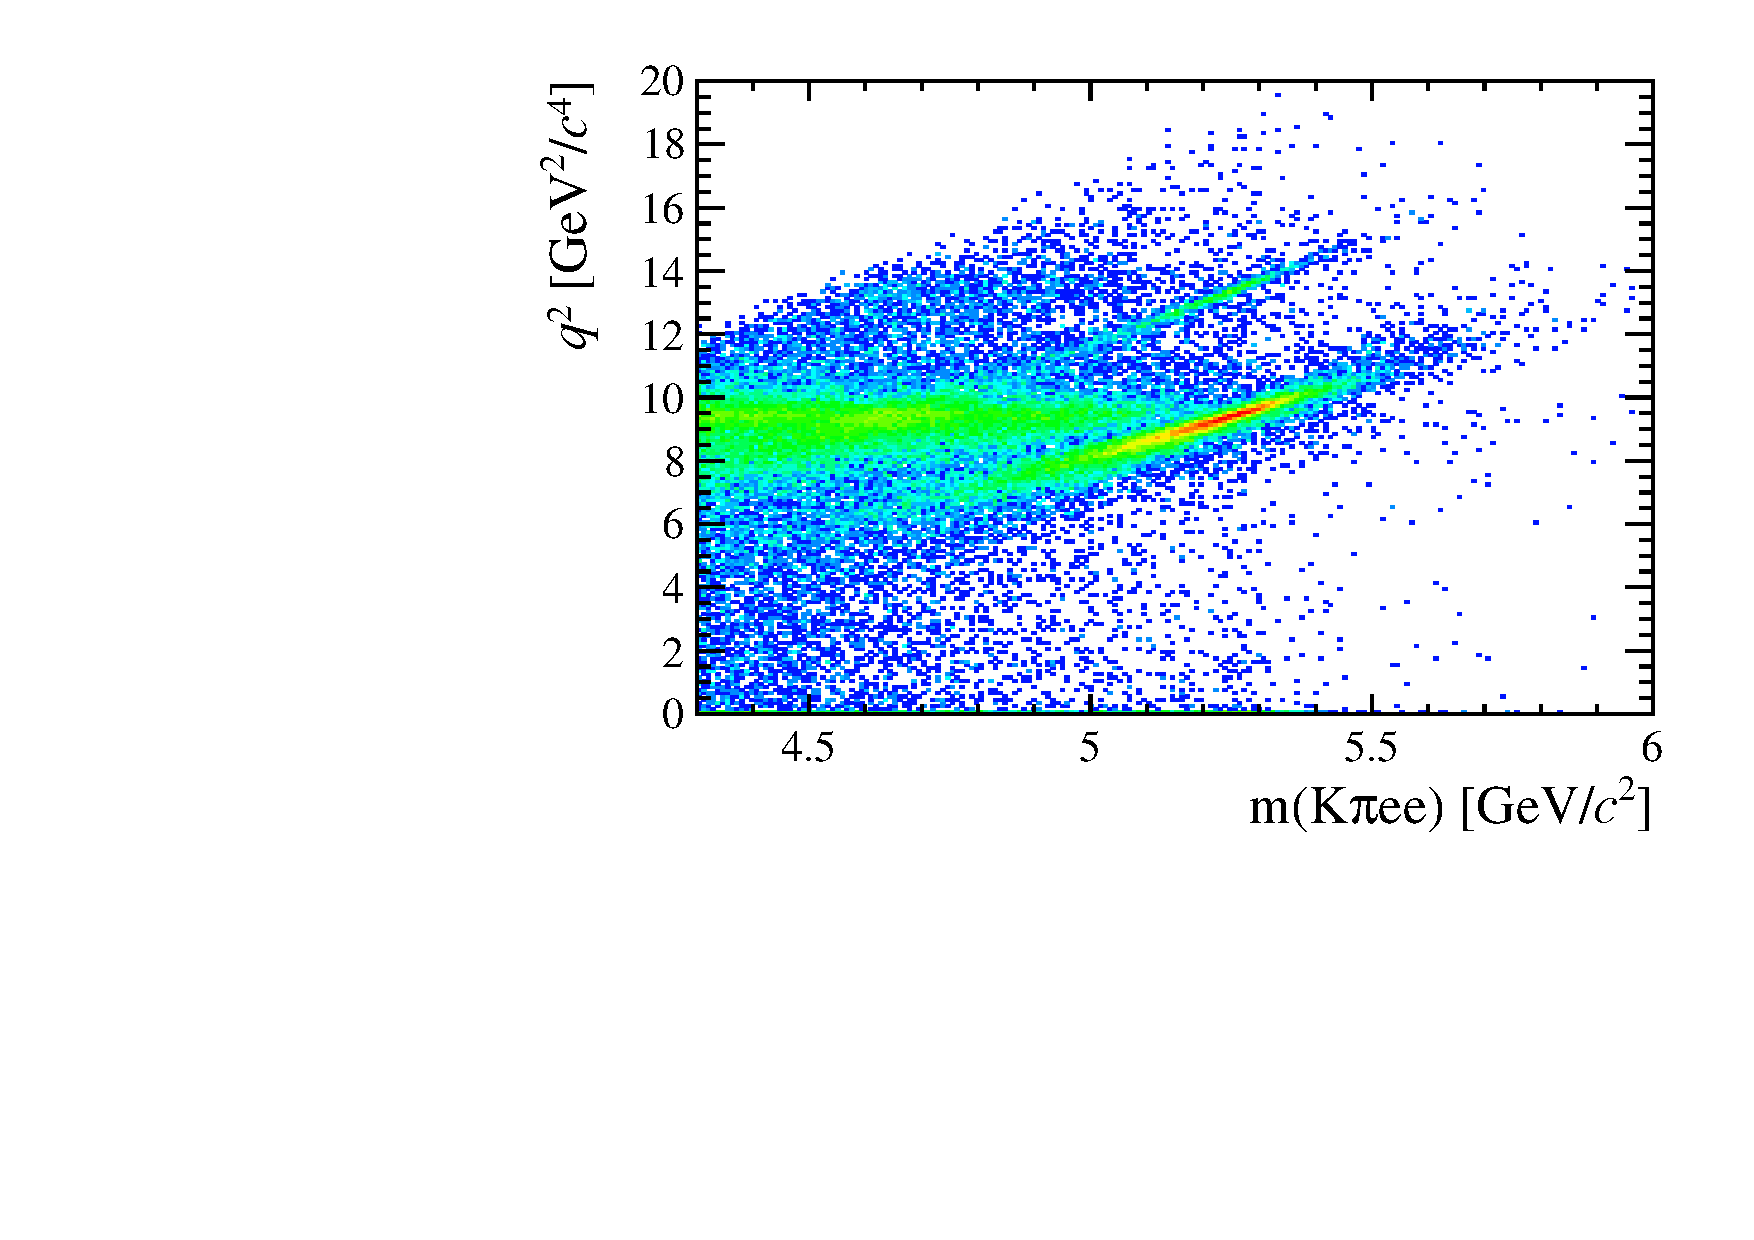
\includegraphics[width=1.\textwidth]{RKst/figs/electron_B0jpsi2D_selected.pdf}
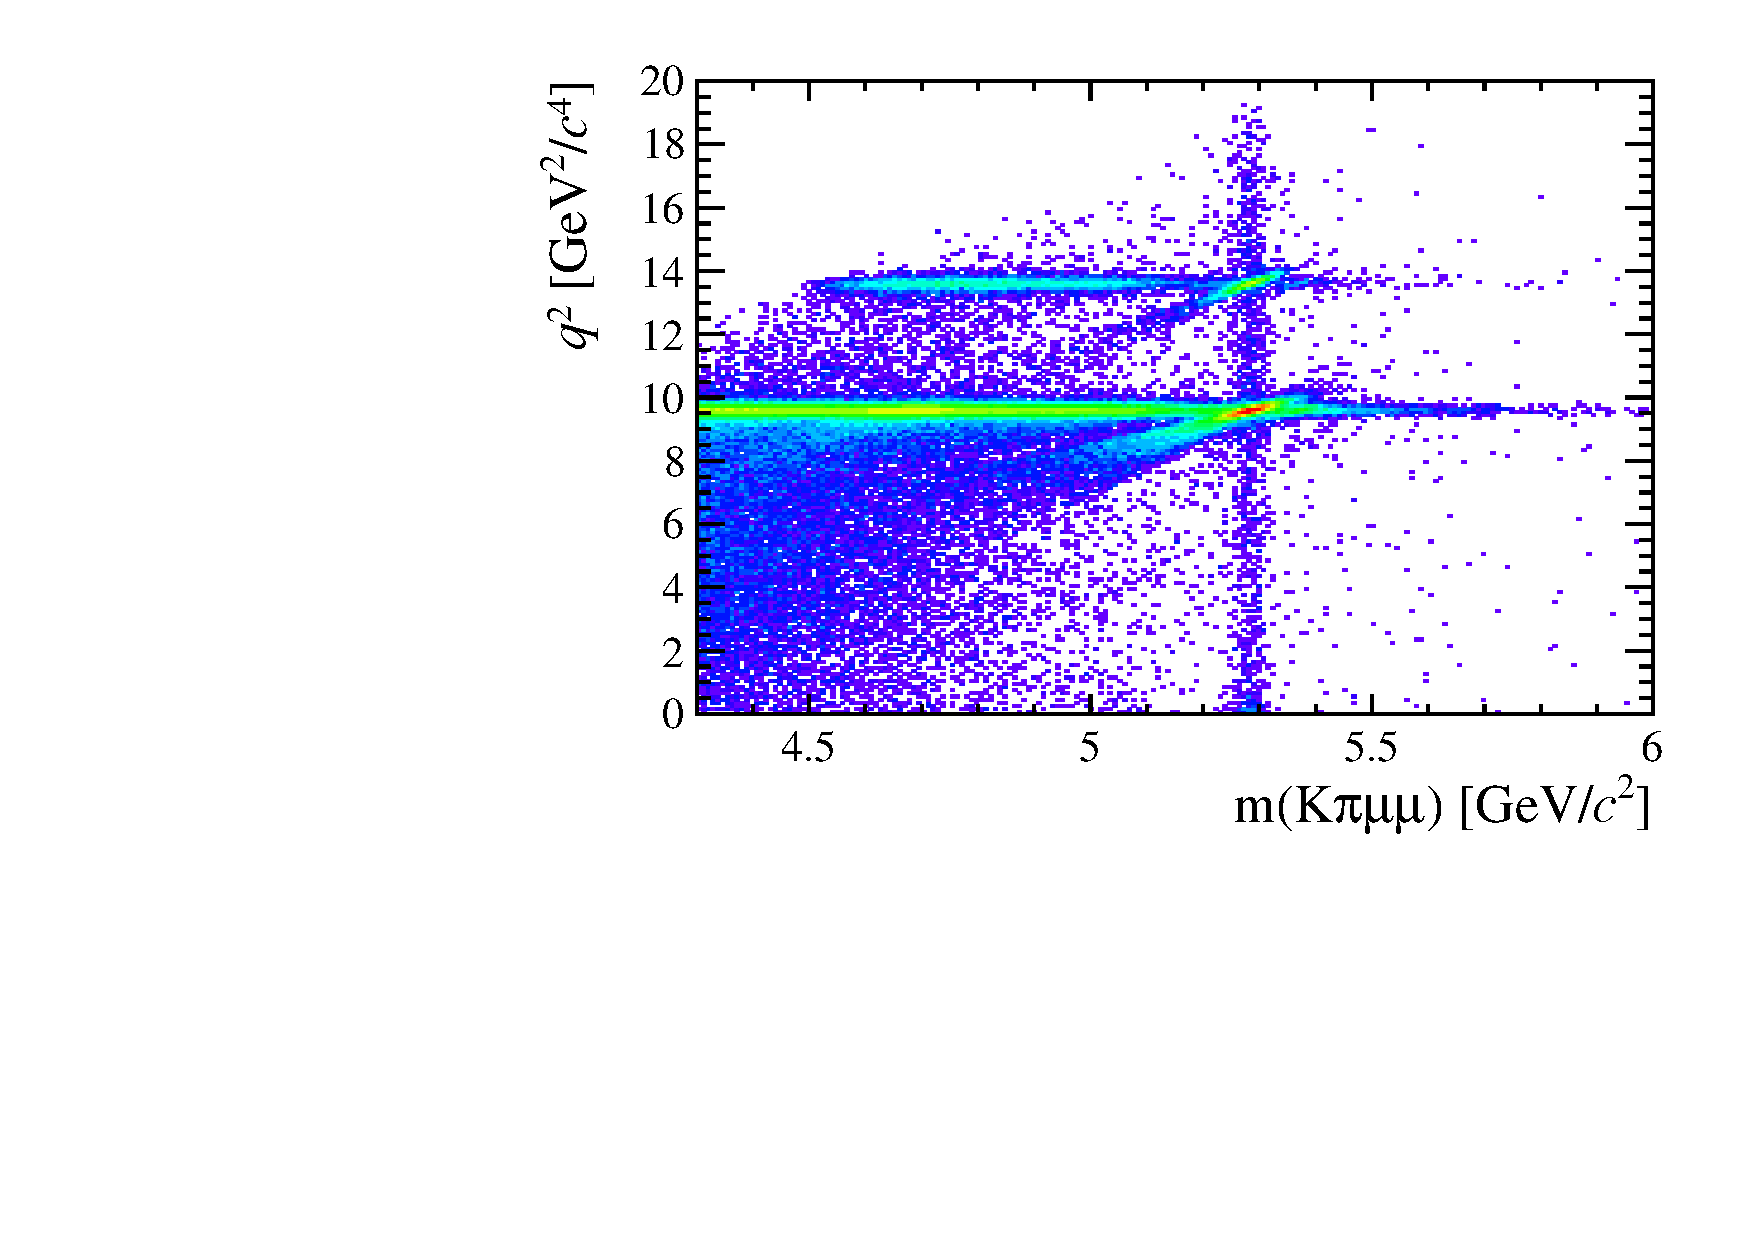
\includegraphics[width=1.\textwidth]{RKst/figs/muon_B0jpsi2D_selected.pdf}
\caption{Two-dimensional \qsq versus $m(K\pi\ell\ell)$ distributions for 
fully selected electron (top) and muon (bottom) candidates in 2012 data. 
Requirements on \qsq to separate the various decay channels are not applied.}
\label{fig:2D_q2_B0mass}
\end{figure}

\begin{table}[t!]
\begin{center}
\caption{Summary of the channel categories.}
\label{tab:candidates}
\begin{footnotesize}
\renewcommand\arraystretch{1.4}
\begin{tabular}{$c|^c|^c}
\rowstyle{\bfseries}
 Type & Sample & \boldmath{\qsq} \\
\hline
\multirow{4}{*}{$\mu\mu$}
	& \BdToKstmm (low)			& $0.0004<\qsq<1.1\gevgevcccc$ \\
	& \BdToKstmm (central)		& $1.1<\qsq<6\gevgevcccc$ \\
	& \BdToKstmm (high)		& $\qsq>15\gevgevcccc$ \\
	& \BdToKstJPsmm 			& $|m_{\mu\mu} - m_{\jpsi}^{PDG}| < 100\mevcc$ \\ \hline
\multirow{7}{*}{$ee$} 
	&  \BdToKstee (low)			& $0.0004<\qsq<1.1\gevgevcccc$ \\
	& \BdToKstee (central)		& $1.1<\qsq<6\gevgevcccc$ \\
	& \BdToKstee (high)			& $\qsq>15\gevgevcccc$ \\
	& \BdToKstJPsee 			& $6<\qsq<11\gevgevcccc$ \\
\cline{2-3}
	& \multicolumn{2}{c}{Control samples} \\ \cline{2-3}
	& \BdToKstGee 			& $\qsq<0.0004\gevgevcccc$ \\
%	& \BdToKstJPsee (\mKpiee)	& $6<\qsq<11\gevgevcccc$ \\
	& \BdToKstPsiee 			& $11<\qsq<15\gevgevcccc$ \\
\end{tabular}
\end{footnotesize}
\end{center}
\end{table}


\subsection{Trigger and pre-selection }
\label{sec:RKst_trigstripping}

Events are triggered for the $\mu\mu$ and the $ee$ channels by the trigger lines
reported in Tab.~\ref{tab:RKst_triglines}, where the logical $and$ of L0, HLT1 and HLT2
lines is required and the logical $or$ of the lines on the same level. The candidates are
required to be triggered-on-signal (TOS) for most of the stages, namely it is required that the 
particle responsible for the trigger decision is one of the particles used to build the signal candidates.
Only for \verb!L0Global!, used in the electron case, a trigger-independent-of-signal (TIS) is required. 
%this is aimed to collect all the possible statistics for the electron channels, which are the most challenging.
The \verb!L0Muon! trigger requires hits in the muon detector, while \verb!L0Electron! and \verb!L0Hadron! use information
from the calorimeters; \verb!HLT1TrackAllL0! adds information from the trackers and
triggers if the L0 decision is confirmed; finally, \verb!HLT2Topo[2,3]BodyBBDT! uses a full reconstruction 
of the event and a neural network trained on candidates with a specific topology in order to detect specific decay structures.
%More information about the muon triggers can be found at Sec.~\ref{sec:Lb_trigger}.

\begin{table}[h!]
\begin{center}
\caption{Summary of the trigger lines used to select the $\mu\mu$ and the $ee$ channels.
Where not explicitly indicated, the lines are required to be TOS.}
\begin{tabular}{$c|^c|^c}
\rowstyle{\bfseries}
Trigger level & \boldmath{$\mu\mu$} candidates &  \boldmath{$ee$} candidates \\
\hline
\multirow{3}{*}{L0}     & 	\multirow{3}{*}{L0Muon}		&    	L0Electron	\\
				&							& 	L0Hadron\\
				&							& 	L0Global (TIS)\\
\hline
\multirow{2}{*}{HLT1}		&	Hlt1TrackAllL0				& \multirow{2}{*}{Hlt1TrackAllL0} \\
					&	Hlt1TrackMuon				&	 \\
\hline
\multirow{3}{*}{HLT2}		&	Hlt2Topo[2,4]BodyBBDT 		& Hlt2Topo[2,4]BodyBBDT \\
					& 	Hlt2TopoMu[2,4]BodyBBDT 	& Hlt2TopoE[2,4]BodyBBDT \\
					& 	Hlt2DiMuonDetachedDecision	&							\\
\end{tabular}
\label{tab:RKst_triglines}
\end{center}
\end{table}

For the electron channels the L0 lines have different properties, therefore the analysis 
is performed separately for three categories of events, depending on the L0 trigger that 
accepted them. These categories are defined to be exclusive as:
%in the following way:
%
\begin{itemize}
\item {\bf L0E}: events triggered by at least one of the electrons in the signal candidate: (\verb!L0Electron_TOS!);
\item {\bf L0H}: events triggered by at least one of the hadrons in the signal candidate and not in the L0E category: \\
 (\verb|L0Hadron_TOS && !L0Electron_TOS|);
\item {\bf L0I}: events triggered by particles independent of any signal candidate and not included in the previous categories: \\
(\verb|L0Global_TIS && !(L0Electron_TOS |\verb!|| L0Hadron_TOS)!).
\end{itemize}

The majority of the selected events falls into the L0E category, while
the L0H category is more efficient at low \qsq were the \Kstarz has higher momentum.
Because L0I is defined to be independent of the signal candidate, the corresponding
signal efficiency is the same in both the rare and resonant cases and therefore cancels in their ratio.

Candidates are then required to pass the kinematic and quality cuts summarised in Tab.~\ref{tab:RKstripping},
where the meaning of the variables was already explained in Sec.~\ref{sec:Lb_selection}.
Loose PID requirements are applied in the pre-selection to limit the size of the samples, while tighter cuts 
are applied in a second stage. A wide mass window is kept around the \Bz peak so that
 the sideband can be used to train the multivariate classifier and to better constrain the backgrounds in the fit.
%
%In the table $IP_{\chi_2}$ is defined as the projected distance from the vertex divided by its uncertainty, for example $IP^B_{\chi_2}(primary) > 4$ means
%that the B vertex is 2 standard deviations away from the primary vertex.
%Another quantity used is a pointing variable defined as the angle between the direction of the particle momentum and the flight direction from its mother vertex, called DIRA.
%This allows the selection of particles with well-defined primary vertices.
%%$GhostProb$ is the probability, estimated from the reconstruction algorithm, for the track to be a ghost. 
%Loose PID cuts are applied in preselection to limit the size of the samples, while tighter cuts are applied
%in a second stage. To quantify the PID of a particle the pion is used as a reference point and a Log-Likelihood
%variable is used. Therefore the {\verb PID } variable reported in the table is given in terms of the difference between
%the Log-Likelihood of the particle of a given type and a pion. This is called Delta Log-Likelihood (DLL).
%For example:
%\begin{equation}
%\verb!PID!_K = \text{DLL}_{K-\pi} = \log(\mathcal{L}_K) - \log(\mathcal{L}_\pi)
%\end{equation}
%
\begin{table}[]
\begin{center}
\caption{Summary of pre-selection requirements. Variables are defined in Sec.~\ref{sec:Lb_selection}. }
\begin{tabular}{$c^c}
\rowstyle{\bfseries}
Particle &  Requirements \\
\hline
%\multirow{2}{*}{ All final}
%       			&   track $\chi_2/\text{ndf} < 3$ \\
%       			&   {\verb GhostProb } $< 0.4$ \\
%\hline
$\pi$			& $\chisqip(primary) > 9$ \\      			
\hline
\multirow{3}{*}{K}
      			& {\verb PID }$_K > -5$ \\
       			& $\chisqip(primary) > 9$ \\
       			& {\verb hasRICH }  \\
 \hline
\multirow{4}{*}{ \Kstarz }
       			& $\pt > 500$ \mevc \\
       			& $|m_{K\pi} - m_{\Kstarz}^{PDG}| < 300$ \mevcc  \\ %300 in stripping but then we restrict it to 100
       			& $\chisqip(primary) > 9$ \\
       			& $\chisq_{vtx}/\text{ndf} < 25$ \\
\hline
\multirow{3}{*}{ $\mu$ }
       			& $\pt > 300$ \mevc \\
       			& $\chisqip(primary) > 9$ \\
       			& {\verb isMuon }\\  %RequiresDet='MUON'
%       		& hasMuon \\
\hline
\multirow{4}{*}{ $e$ }
       			& $\pt > 300$ \mevc \\
       			& $\chisqip(primary) > 9$ \\
       			& {\verb hasCalo }\\ %RequiresDet='CALO'
       			& \verb!PID!$_e > 0$ \\
\hline
\multirow{4}{*}{ $\ell\ell$ }
				& $m_{\ell\ell} < 5500$ \mevcc \\
			  	& $\chisq_{vtx}/\text{ndf} < 9$ \\
			  	& $\chisq_{\rm FD} > 16$ \\
%			  	& $\chisqip(primary) > 0$ \\
\hline
\multirow{4}{*}{ $B^0$  }
 %      & $| m - m_{B^0}^{PDG}| < 600$ \mevcc  \\
       			& {\verb DIRA } $> 0.9995$ \\ 
       			& $\chisq_{vtx}/\text{ndf} < 9$ \\
     			& $\chisqip(primary) < 25$ \\
     			& $\chisq_{\rm FD} > 100$ \\
\end{tabular}
\label{tab:RKstripping}
\end{center}
\end{table}
%
Track and vertex quality cuts are also applied using the $\chisq_{trk}$, 
{\verb GhostProb }, and $\chisq_{vtx}$
variables. The {\verb GhostProb } quantity describes the probability of a track being fake.
By construction, cutting at 0.4 removes $(1 - 0.4)\cdot 100 = 60\%$ of fake tracks.
For details about the definition of the variables used see Ref.~\cite{Loki_twiki}.

\subsection{PID}
\label{sec:PID}

After pre-selection there still are high levels of background.
In particular, as the identification (ID) hypotheses for kaons and pions are not constrained, 
the samples still contain multiple ID combinations for most candidates, therefore, tighter PID requirements are applied.
In LHCb the particle identification probability can be quantified using the ``{\verb ProbNN }" variables~\cite{ProbNNs_pres}. 
A separate {\verb ProbNN }$x$ variable is defined for each ID hypothesis, $x$: $p$, $K$, $\pi$, $e$ or $\mu$. 
These variables are the outputs of neural networks which use information from the calorimeters, the RICH detectors
the muon system and the tracking system. Unlike the DLL variables (see Sec.~\ref{sec:PID_perf})
the {\verb ProbNN } are bound from 0 to 1 and can be directly interpreted as probabilities; \emph{e.g.}
 {\verb ProbNNk } corresponds to the probability for a reconstructed particle to be a kaon.
%Two tunes of the {\verb ProbNN } variables, labelled V2 and V3, are available.
%Tune V3 was shown to be optimal for positive ID, while tune V2 was found to be optimal
%for background rejection and therefore it is used to quantify the mis-ID probability.
%
\begin{figure}[h!]
\centering 
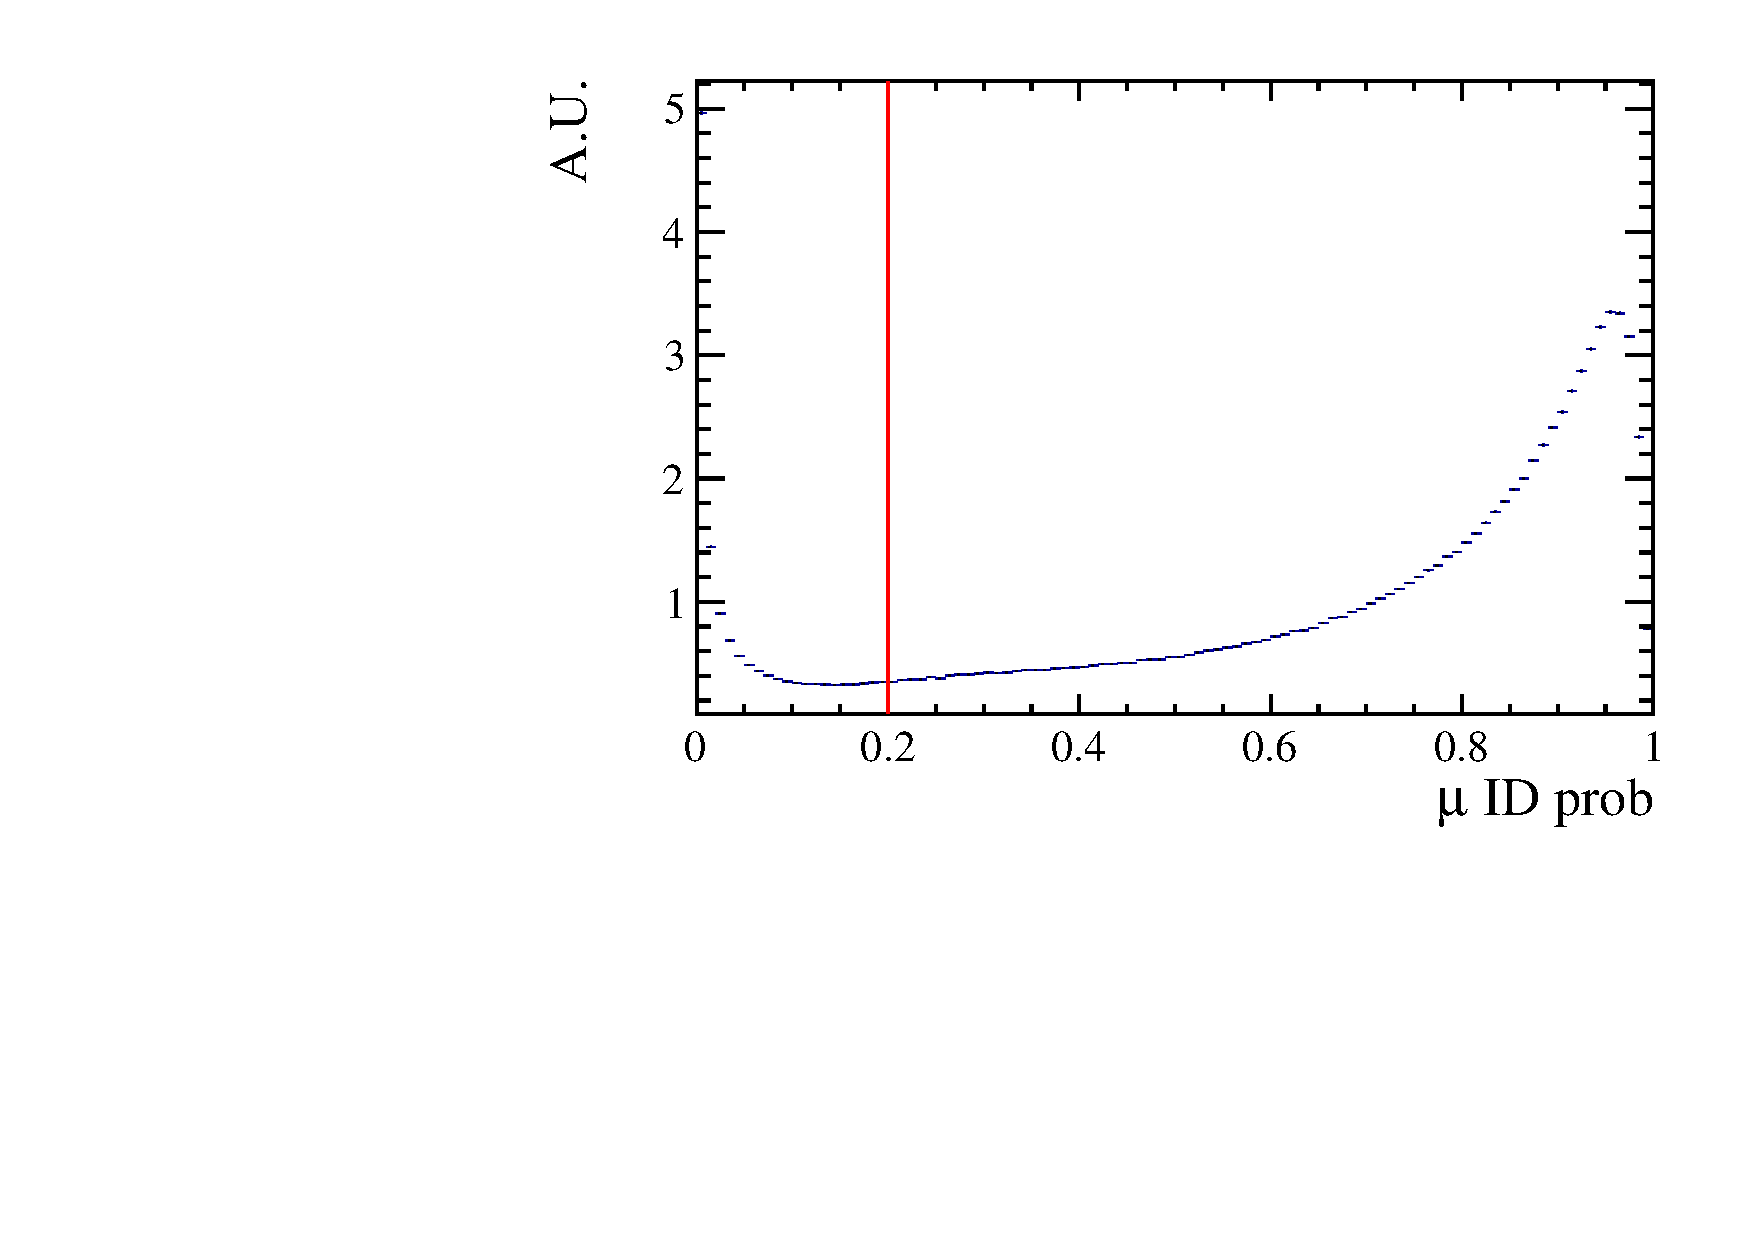
\includegraphics[width=0.49\textwidth]{RKst/figs/muon_PID.pdf}
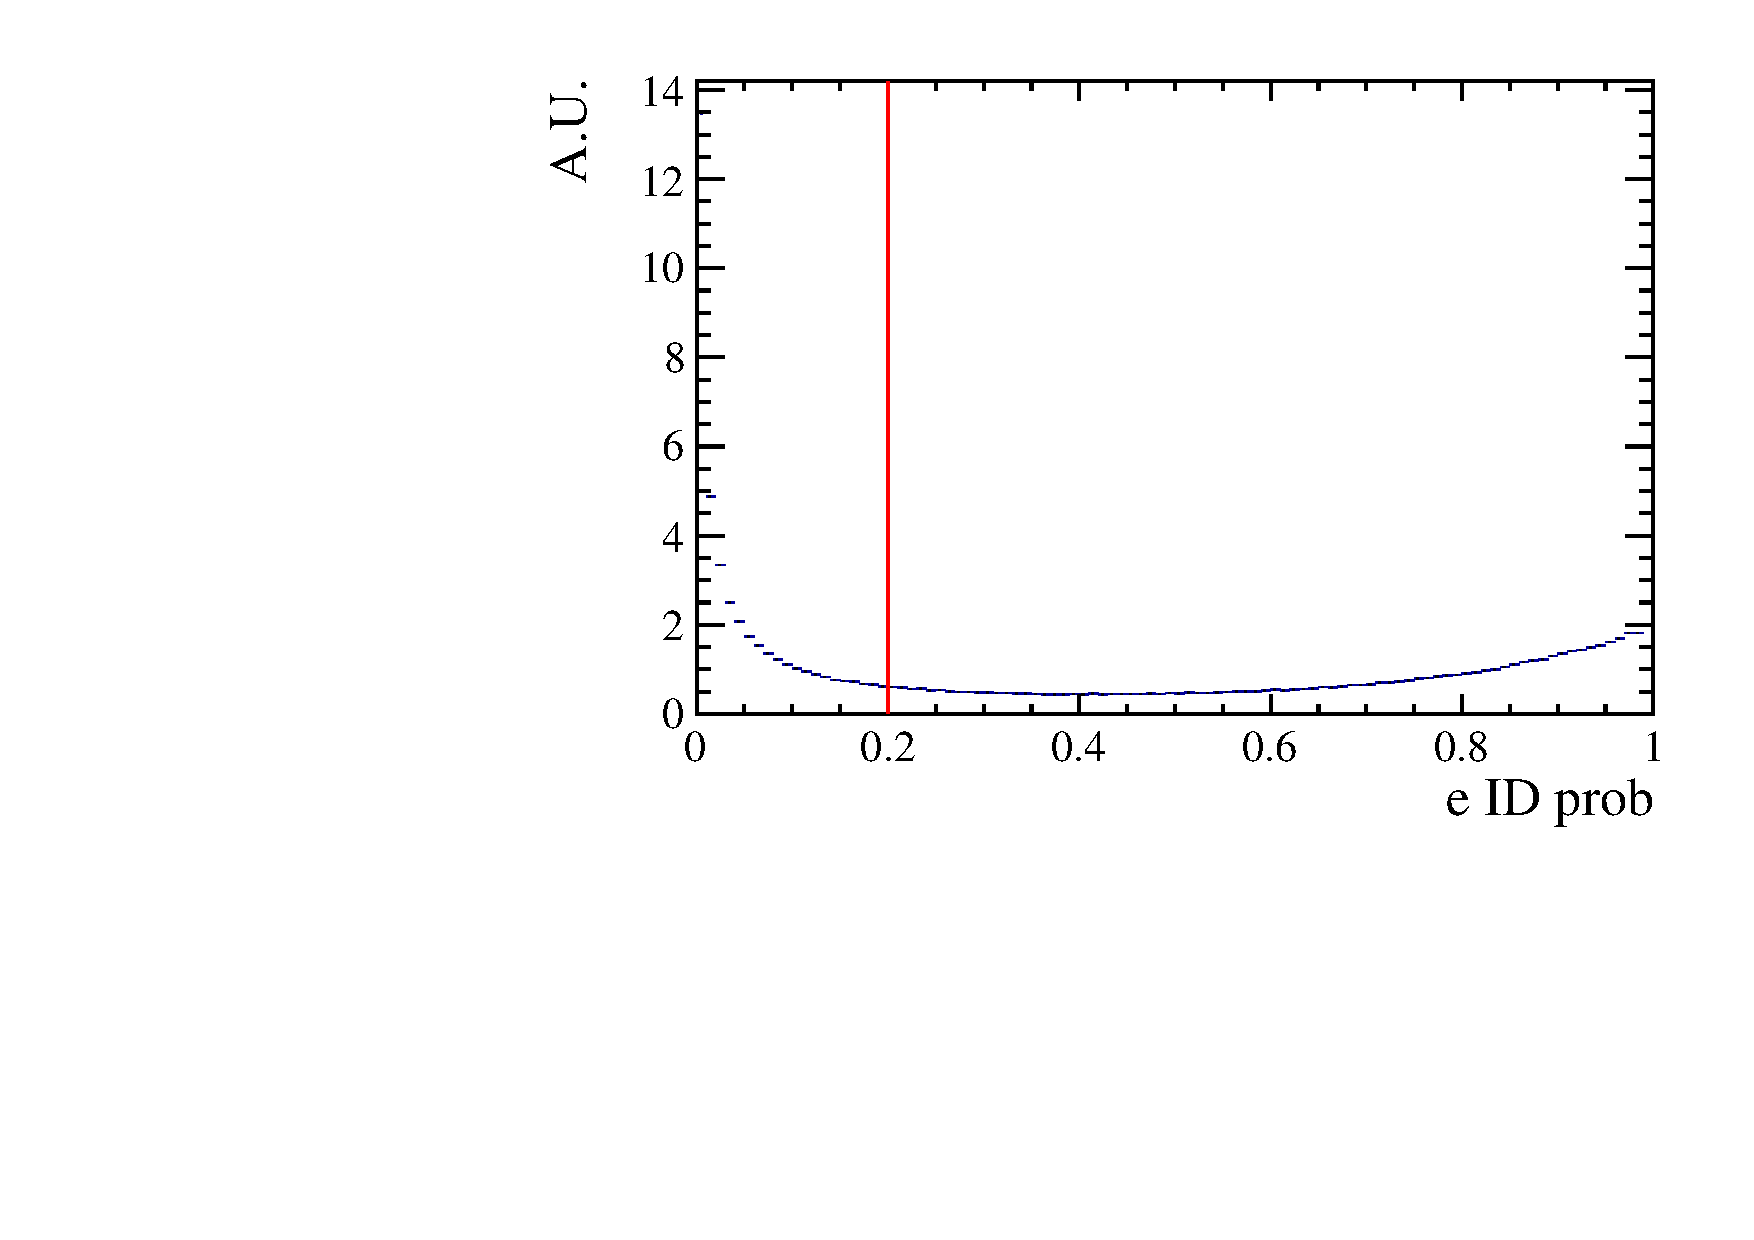
\includegraphics[width=0.49\textwidth]{RKst/figs/electron_PID.pdf}
\caption{Correct ID probability distributions for muons (left)
and electron (right) in 2012 data. The red line indicates the chosen cut.}
\label{fig:e_mu_pid}
\end{figure}
%
\begin{figure}[h!]
\centering 
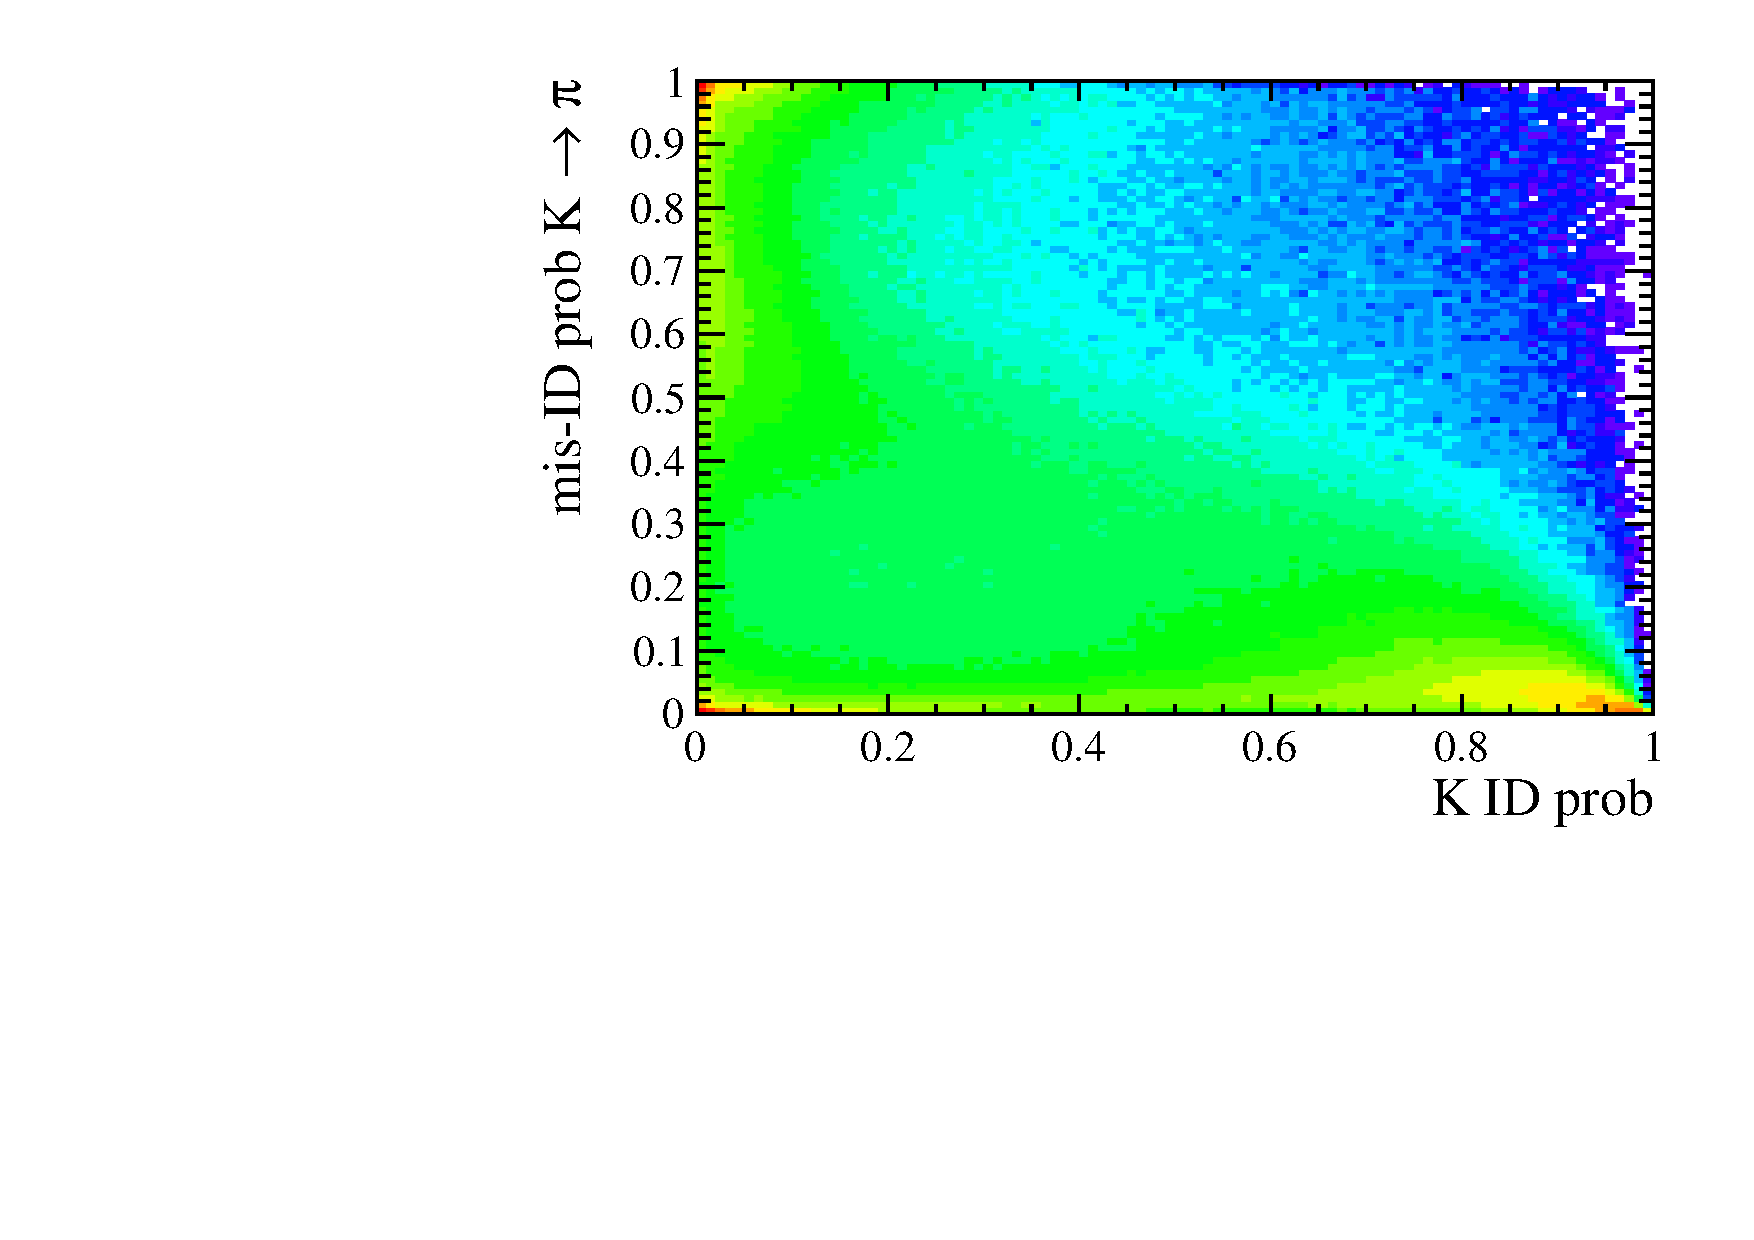
\includegraphics[width=0.49\textwidth]{RKst/figs/kaon_PID.pdf}
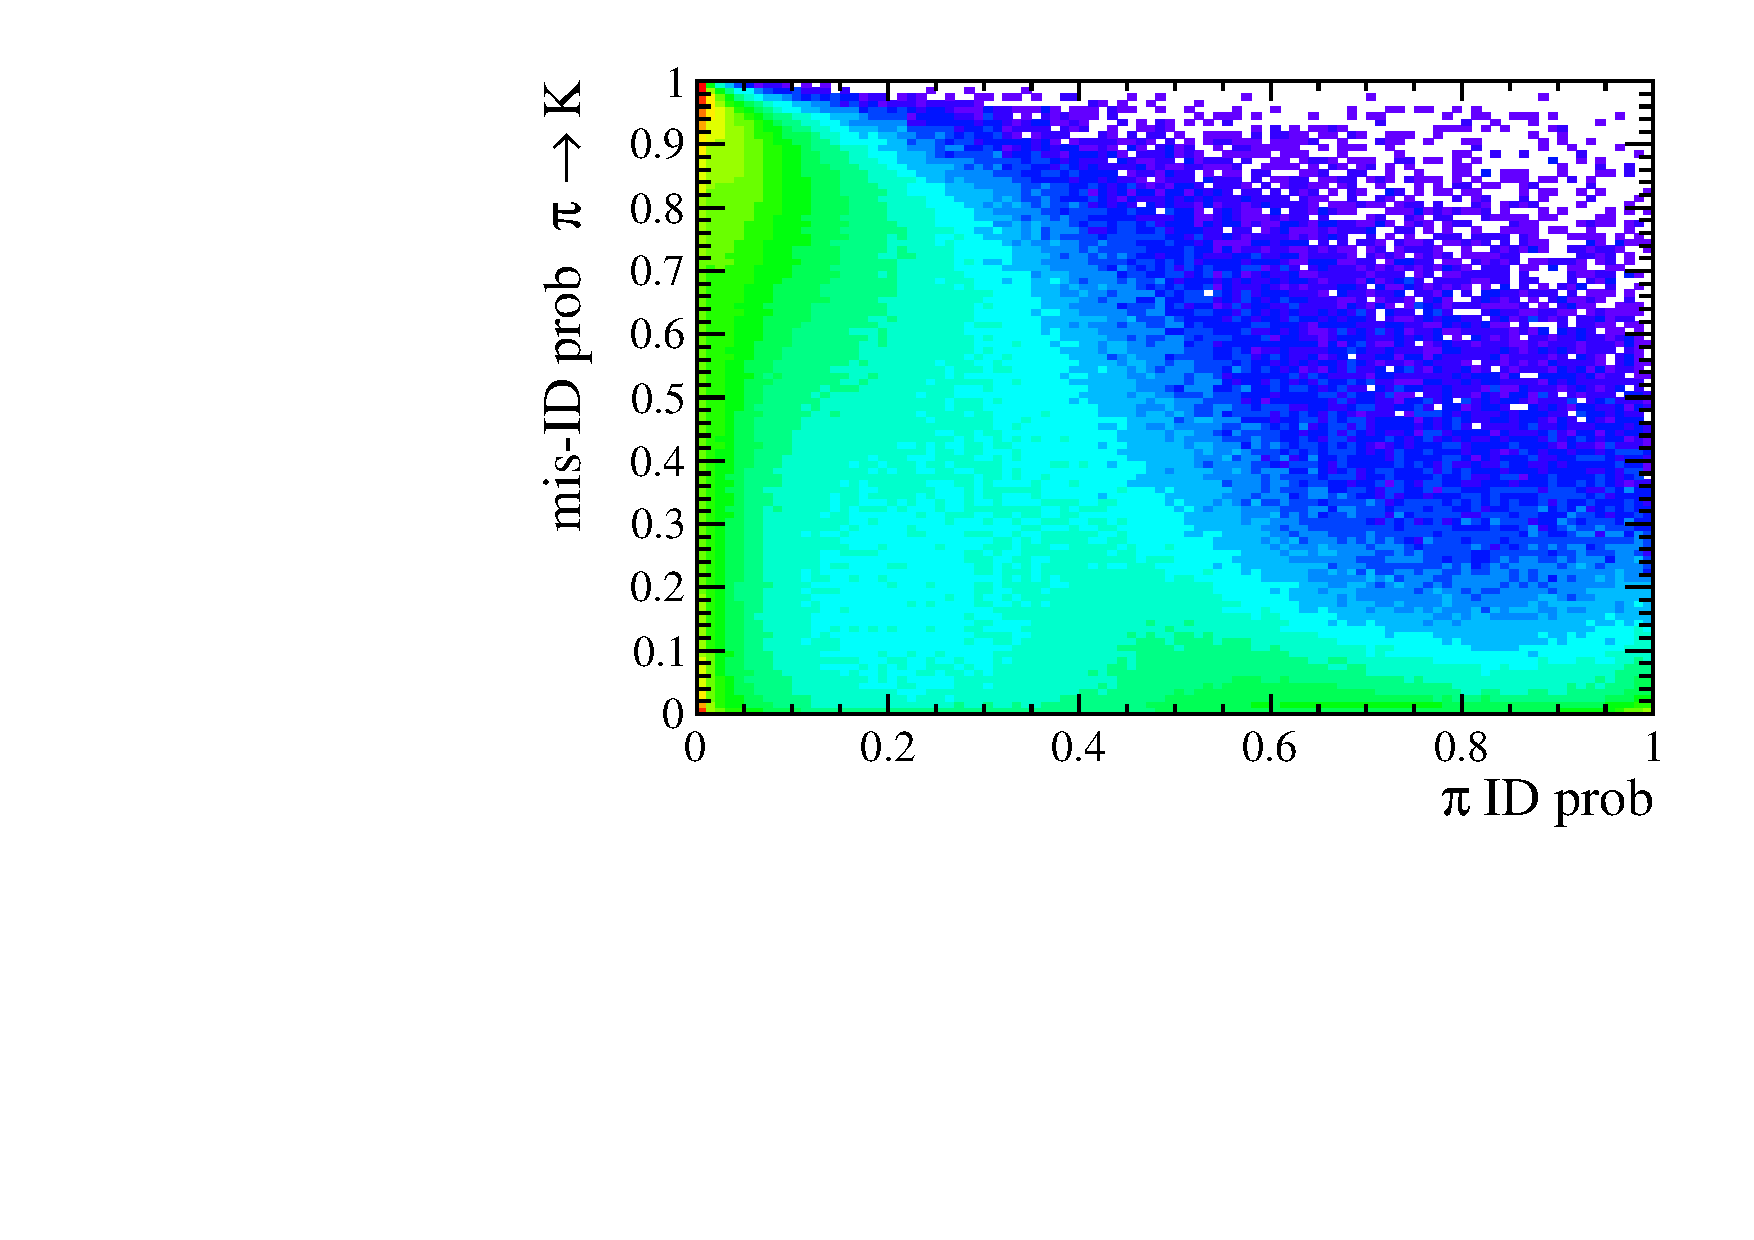
\includegraphics[width=0.49\textwidth]{RKst/figs/pion_PID.pdf}
\caption{Correct ID versus mis-ID probability distributions for 
the kaon (left) and the pion (right) in the decay candidates after pre-selection.}
\label{fig:k_pi_pid}
\end{figure}

Figure~\ref{fig:e_mu_pid} shows probability distributions, {\verb ProbNNe } and {\verb ProbNNmu },
for the electrons and muons in the decay candidates, while Fig.~\ref{fig:k_pi_pid} shows the probabilities 
of correct identification and mis-identification of kaons and pions in a two-dimensional plane.
These plots are characterised by clear peaks at maximal ID probability and minimal mis-ID
probability, corresponding to particles to which a well defined identification can be assigned.
%
In order to maximise the power of the PID requirements, the probabilities for correct ID 
and mis-ID are combined and requirements imposed as:
%
\begin{center}
\begin{tabular}{lcl}
$\pi$     & \to  & $\verb!ProbNNpi! \times (1 - \verb!ProbNNk!) \times (1 - \verb!ProbNNp!) > 0.1$ \\
$K$      & \to  & $\verb!ProbNNk! \times (1 - \verb!ProbNNp! ) > 0.05$ \\ 
$\mu$  & \to  & $\text{min}(\verb! ProbNNmu!(\mu_1) , \verb! ProbNNmu!(\mu_2)\;) > 0.2$  \\
$e$      & \to  & $\text{min}(\verb! ProbNNe!(e_1), \verb! ProbNNe!(e_2)\;) > 0.2$ \\
%$\pi$ &\to  & $\verb!ProbNNpi-V3! \times (1 - \verb!ProbNNk-V2!) \times (1 - \verb!ProbNNp-V2!) > 0.1$ \\
%$K$   &\to  & $\verb!ProbNNk-V3! \times (1 - \verb!ProbNNp-V2! ) > 0.05$ \\ 
%$\mu$ &\to  & $\text{min}(\verb! ProbNNmu-V3! , \verb! ProbNNmu-V3 !) > 0.2$  \\
%$e$   &\to  & $\text{min}(\verb! ProbNNe-V3! , \verb! ProbNNe-V3 !) > 0.2$ \\
\end{tabular}
\end{center}
%
In the first formula, for example, {\verb ProbNNpi } is the probability of correctly identifying the
pion as a pion, while {\verb ProbNNk } is the probability of mistaking it for a kaon.
Therefore by maximising the quantity ``{\verb ProbNNpi } $\times$ (1 - {\verb ProbNNk })",
one can maximise the correct ID probability and minimise at the same time the mis-ID probability.
In this example, the probability for mistaking the pion as a proton is also used.
%In the kaon case we do not use requirements on the $K\to\pi$ mis-ID probability
%because this cut was found to be unacceptably inefficient.


\subsection{Peaking backgrounds }

Backgrounds due to specific decays usually peak in some variable because of their
distinctive kinematic properties and therefore they can be removed without significant
efficiency loss for the signal. The following sections describe the main sources of peaking background.
The same requirements are applied to the muon and electron channels, unless stated otherwise.

\subsubsection{Charmonium vetoes}

Charmonium resonances such as \jpsi and \psitwos peak in \qsq.
The choice of \qsq binning described in Sec.~\ref{sec:RKst_q2_choice}
constitutes a natural veto for these decays. Simulated events are used
to check if resonant candidates leak inside the \qsq intervals chosen for
the rare channel analysis. For the muon channels the leakage is negligible
as the peaks are sharper due to the better momentum resolution and because muons 
emit fewer bremsstrahlung photons, resulting in shorter radiative tails.
In contrast, the electron channels are characterised by a poorer energy resolution and an increased 
radiation of bremsstrahlung photons, yielding long tails at low \qsq.
Analysing simulated events it was found that 1.3 -- 2\% (depending on
the trigger category) of \mbox{$\Bz\to\Kstarz(\jpsi\to\ee)$} candidates leak into the 
$1.1 < \qsq < 6$~\gevgevcccc interval and 1.8\% of \psitwos candidates leak above 
15~\gevgevcccc. The contribution from these candidates is modelled in the fit. 


\subsubsection{$\phi$ veto}

A kaon from the decay $\Bs \rightarrow \phi \ll$, where the $\phi$ decays in two kaons,
can be mis-identified as a pion and therefore cause the $\phi$ to be reconstructed as a $\Kstarz$. This results in
a candidate with a value of $m(K\pi)$ that is less than the nominal \Kstarz mass but still high enough to
pass the selection requirements. Figure~\ref{fig:phiplots} (left) shows a plot of $m(K\pi)$ versus
$m(K\pi \mu\mu)$, where the kaon mass hypothesis is assigned to the pion. A peak can clearly be seen
around the (\Bs,$\phi$) mass.
To remove this background only candidates with $m(K(\pi\rightarrow K)) > 1040$~\mevcc~are selected.
This results in a $\sim98\%$ background rejection while keeping a $\sim99\%$ signal efficiency.
%This cut could be further optimised using PID information. On the other hand LHCb simulation 
%struggles modelling the PID variables correctly. Therefore using PID in these cuts would
%add systematic uncertainties without significantly improving the signal efficiency which is already 99\%.
\Bs decays such as $B_s \rightarrow \phi \Kstarz$ could also constitute a background when the $\phi$ decays 
into two leptons but the branching fraction of this decay is small compared to the previous case.
Furthermore, this contribution is already taken into account by the choice of the \qsq intervals (see Sec.~\ref{sec:RKst_q2_choice}).

\begin{center}
\begin{figure}[h!]
\centering 
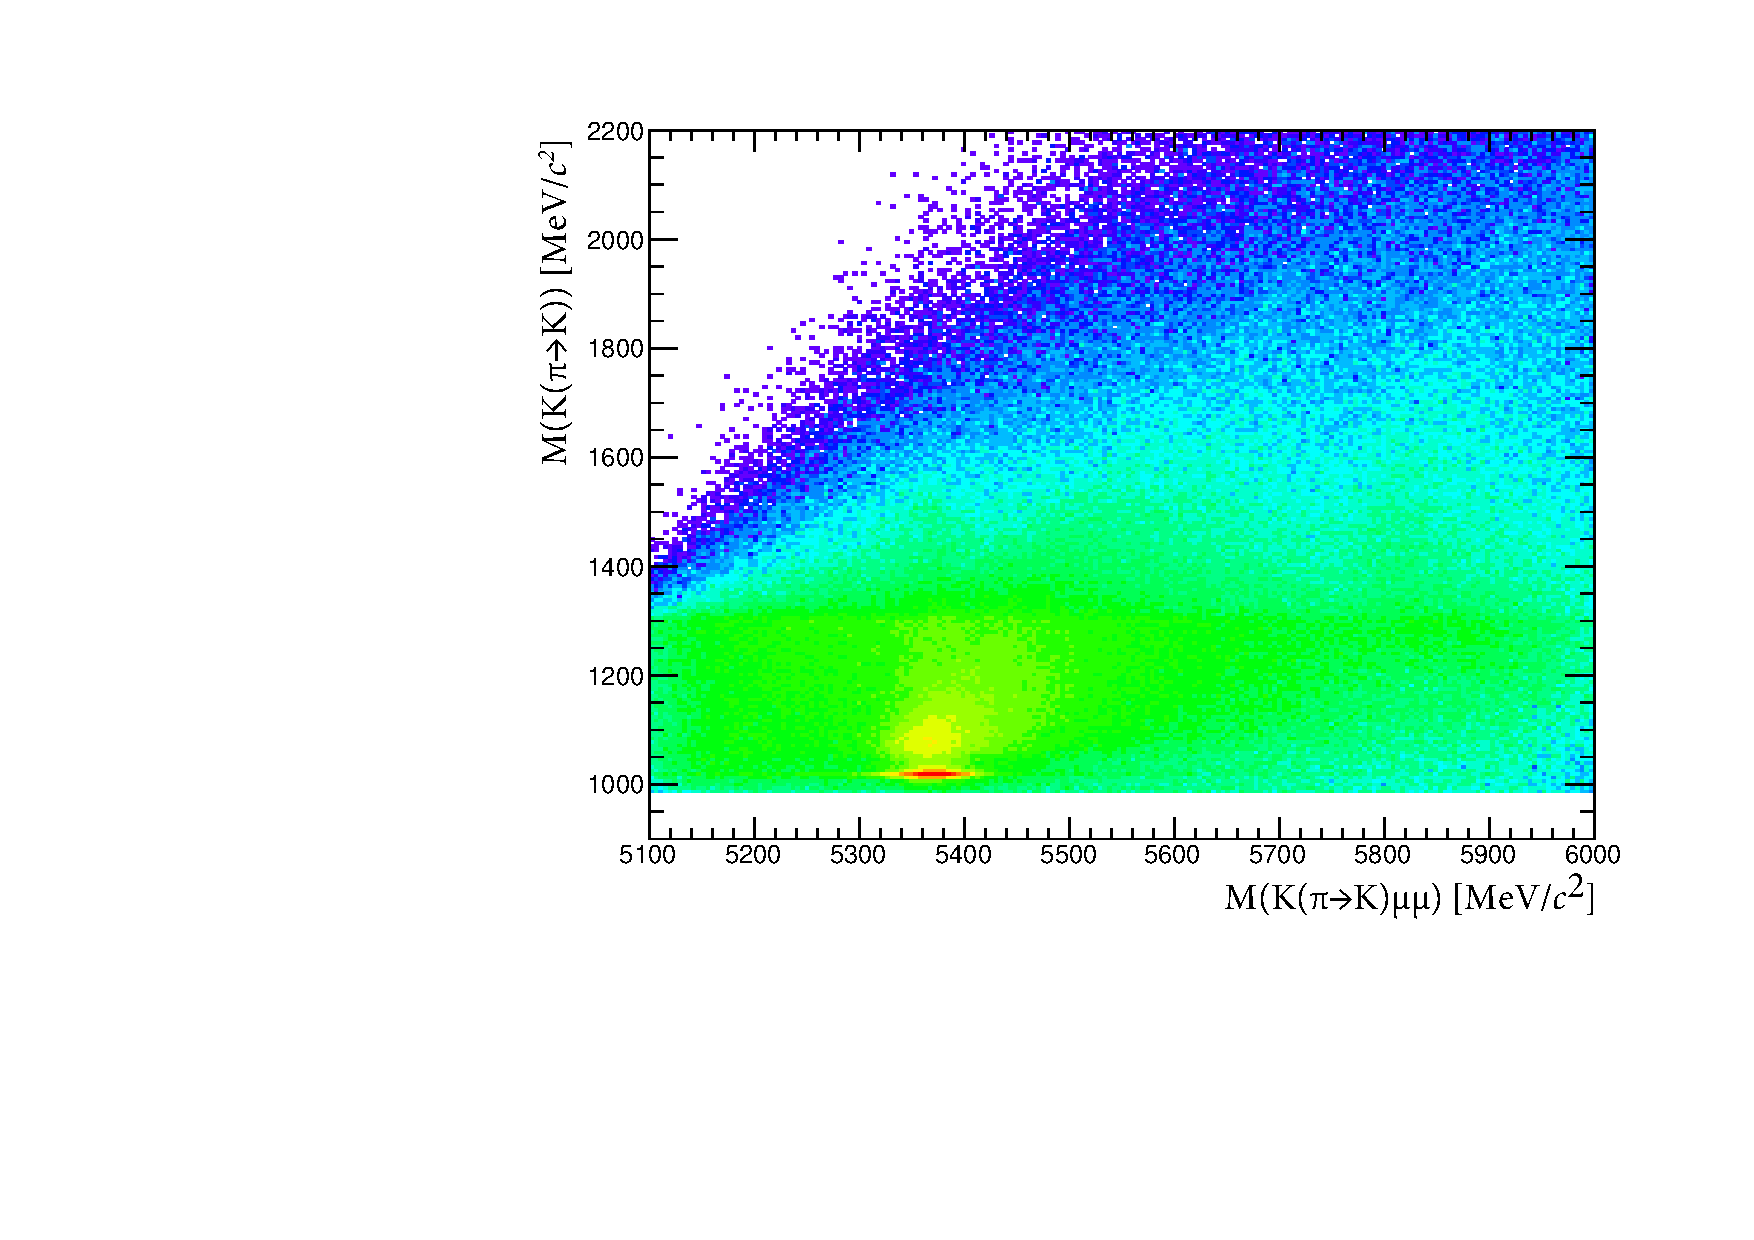
\includegraphics[width=0.49\textwidth]{RKst/figs/Background/phi.pdf}
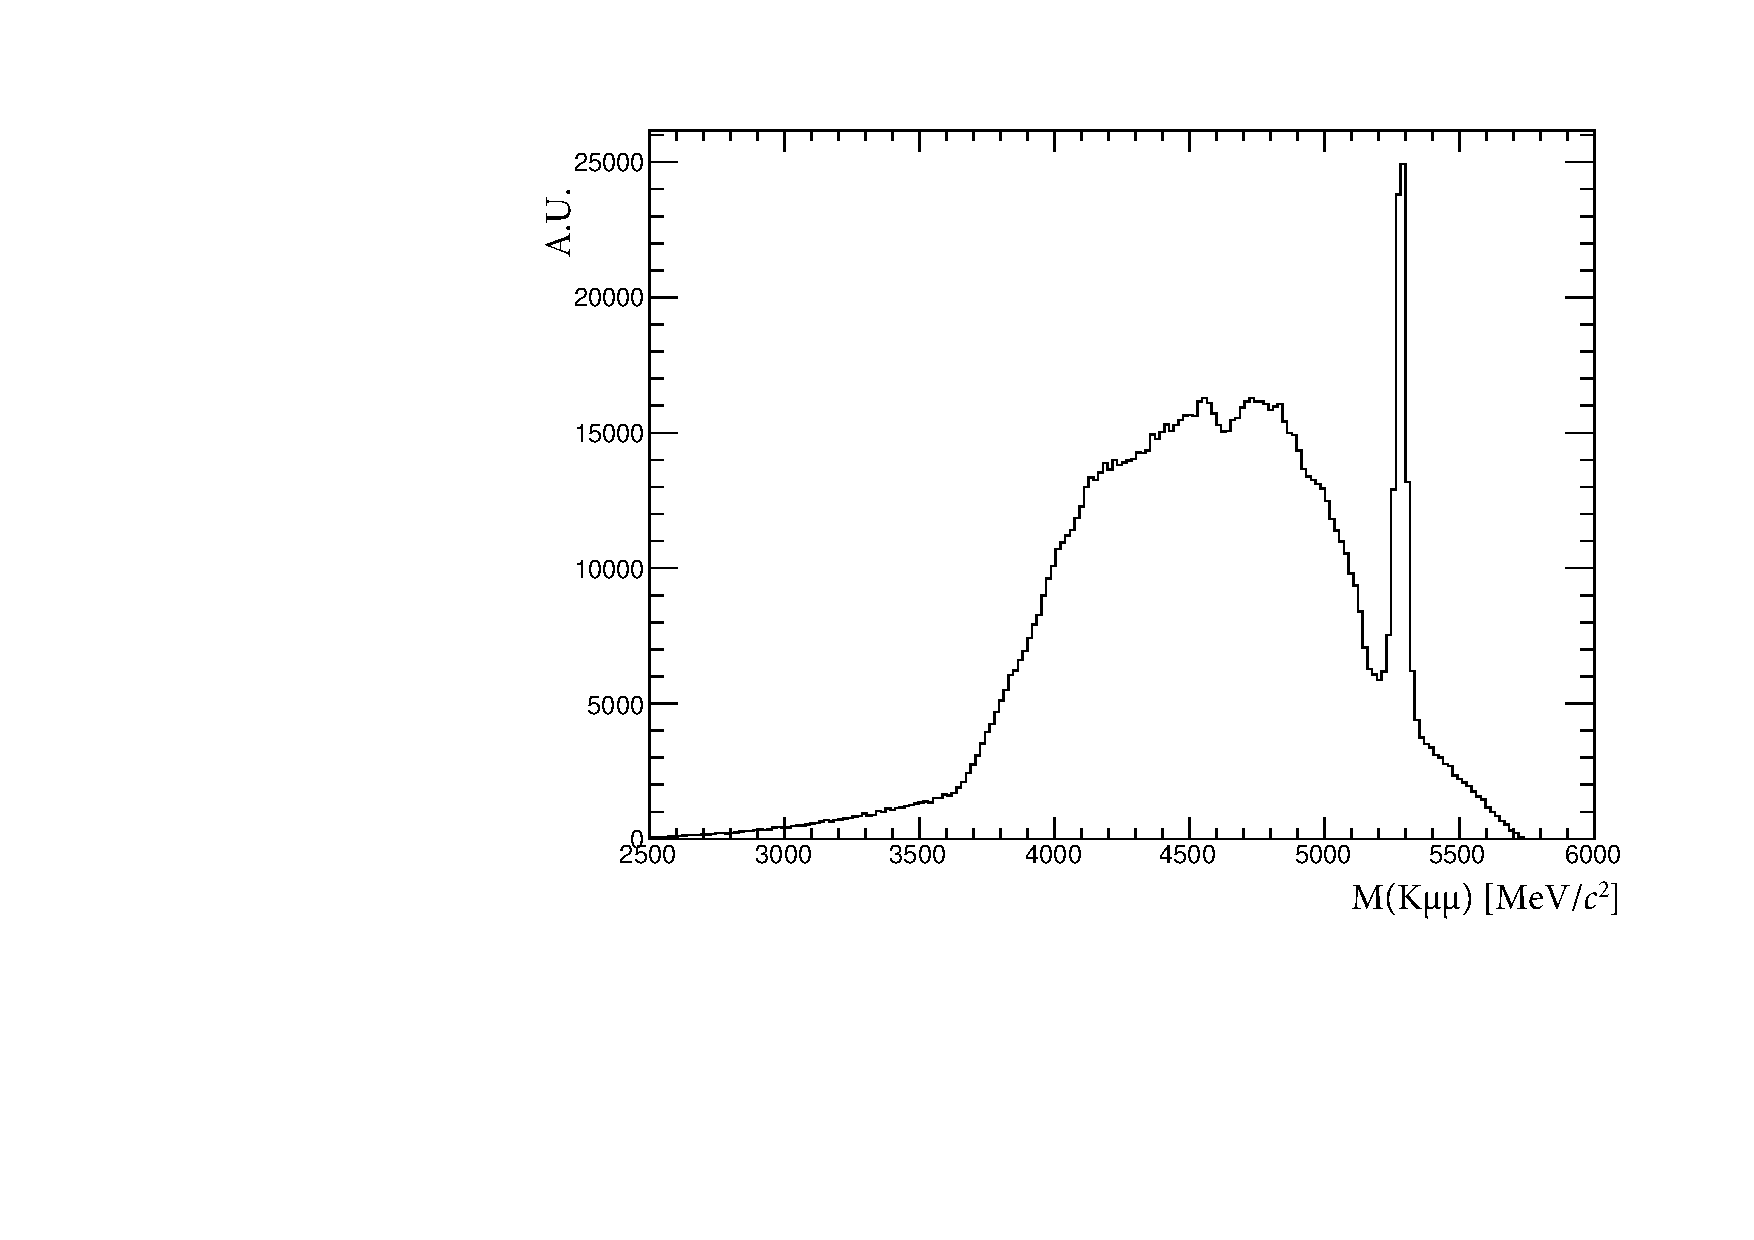
\includegraphics[width=0.49\textwidth]{RKst/figs/Background/Kmumu.pdf}
\caption{ (left) Distribution of data candidates as a function of the variables $m(K(\pi\rightarrow K))$ 
and $m(K(\pi\rightarrow K)\mu\mu)$, where $\pi\rightarrow K$ means that the kaon mass hypothesis 
is assigned to the pion. (right) The invariant mass distribution of the 3-body system $(K\mu\mu)$,
where the peak due to the $B^+ \to K^+ \mumu$ decay is visible. }
\label{fig:phiplots}
\end{figure}
\end{center}


\subsubsection{$\Bu \to K^+ \ll$ plus a random pion}

$\Bu \to K^+ \ll$ decays can contaminate the upper \Bz mass sideband if they are combined
with a soft pion from elsewhere in the event and therefore reconstructed as a \Bz decay.
Similarly, a kaon can be mis-identified as a pion and combined with another kaon in the event.
Figure~\ref{fig:phiplots} (right) shows the invariant mass distribution of the 3-body ($K\mumu$) system,
$m(K\mu\mu)$. This is characterised by a narrow peak at the $\Bu$ mass. Since these
candidates have $m(K\pi\ell\ell) > 5380$~\mevcc~there is no contribution under the \Bz peak,
but they can cause problems when using sidebands candidates to train the neural network.
An effective veto for this decay was found to be max$[m(K\ell\ell),m((K\to\pi)\ell\ell)] < 5.1$~\gevcc,
which results in a $\sim95\%$ background rejection while keeping $\sim99\%$ signal efficiency.

\subsubsection{$\Lambda_b$ decays}

$\Lb\to\jpsi\Lz$ decays are unlikely to be reconstructed as $\Bz \to \Kstarz \ll$ because
the \Lz is long-lived and decays further into the detector with a separate vertex.
%Nevertheless, simulated events were used to check how many 
The number of candidates falling into the \Bz samples was estimated using simulation and found to be negligible. 
In contrast, the $\Lb\to\jpsi pK$ decay channel can contribute more easily, when the proton is mis-identified as a kaon.
In fact, the $m(pK)$ is above the \Lz threshold and therefore they must come from $\Lz^*$ resonances, 
 which are not long-lived. This background is already reduced by the PID requirements but a non-negligible contribution 
 is still expected, and cannot be easily removed due to its broad shape. It is therefore modelled in the fit.

\subsubsection{\decay{\Bd}{(\Dm\to K \en \overline{\nu})\ep\nu} }

The \decay{\Bd}{\Dm\ep\nu} decay, where the \Dm in turn decays semileptonically to $\Kstarz\en\nu$ has the same final particles
as the \BdToKstee decay plus two neutrinos which are not reconstructed. This decay has a branching ratio almost four orders of 
magnitude larger than \BdToKstee and it may pass the selection requirements when the two neutrinos have low momenta. 
%This cut, developed for the angular analysis, 
To reduce the level of this background the angle $\theta_\ell$ is used, which is defined as the angle between the direction of the \ep (\en)
in the dielectron rest frame and the direction of the dielectron in the \Bd (\Bdb) rest frame. 
Low momentum neutrinos demand the \Dm and the \ep to be almost back-to-back in the \Bd rest frame giving the \ep a relatively
high energy compared to the \en. As a consequence, the direction of the \ep is close to the direction of the dielectron pair, thus the
$\theta_\ell$ angle is close to zero. In fact the distribution of background candidates, obtained imposing the invariant mass cut
$m(K\pi ee) < 4800$~\mevcc, is asymmetric towards extreme $\cos \theta_\ell$ values as it can be seen in 
Fig.~\ref{fig:Denu_background}. The requirement $|\cos \theta_\ell\,|< 0.8$ is used to reduce this background but 
it is not applied in the high-\qsq case as the variable loses its discriminating power.
%The percentage of \BdToeeKst signal events lost applying this cut is quite low, about $10\%$ according to MC. 
In the muon channels, the background from \decay{\Bd}{(\Dm\to K \mun \overline{\nu})\mup\nu} decays remains outside 
of the invariant mass window used for the fits.

\begin{figure}[t!]
\centering
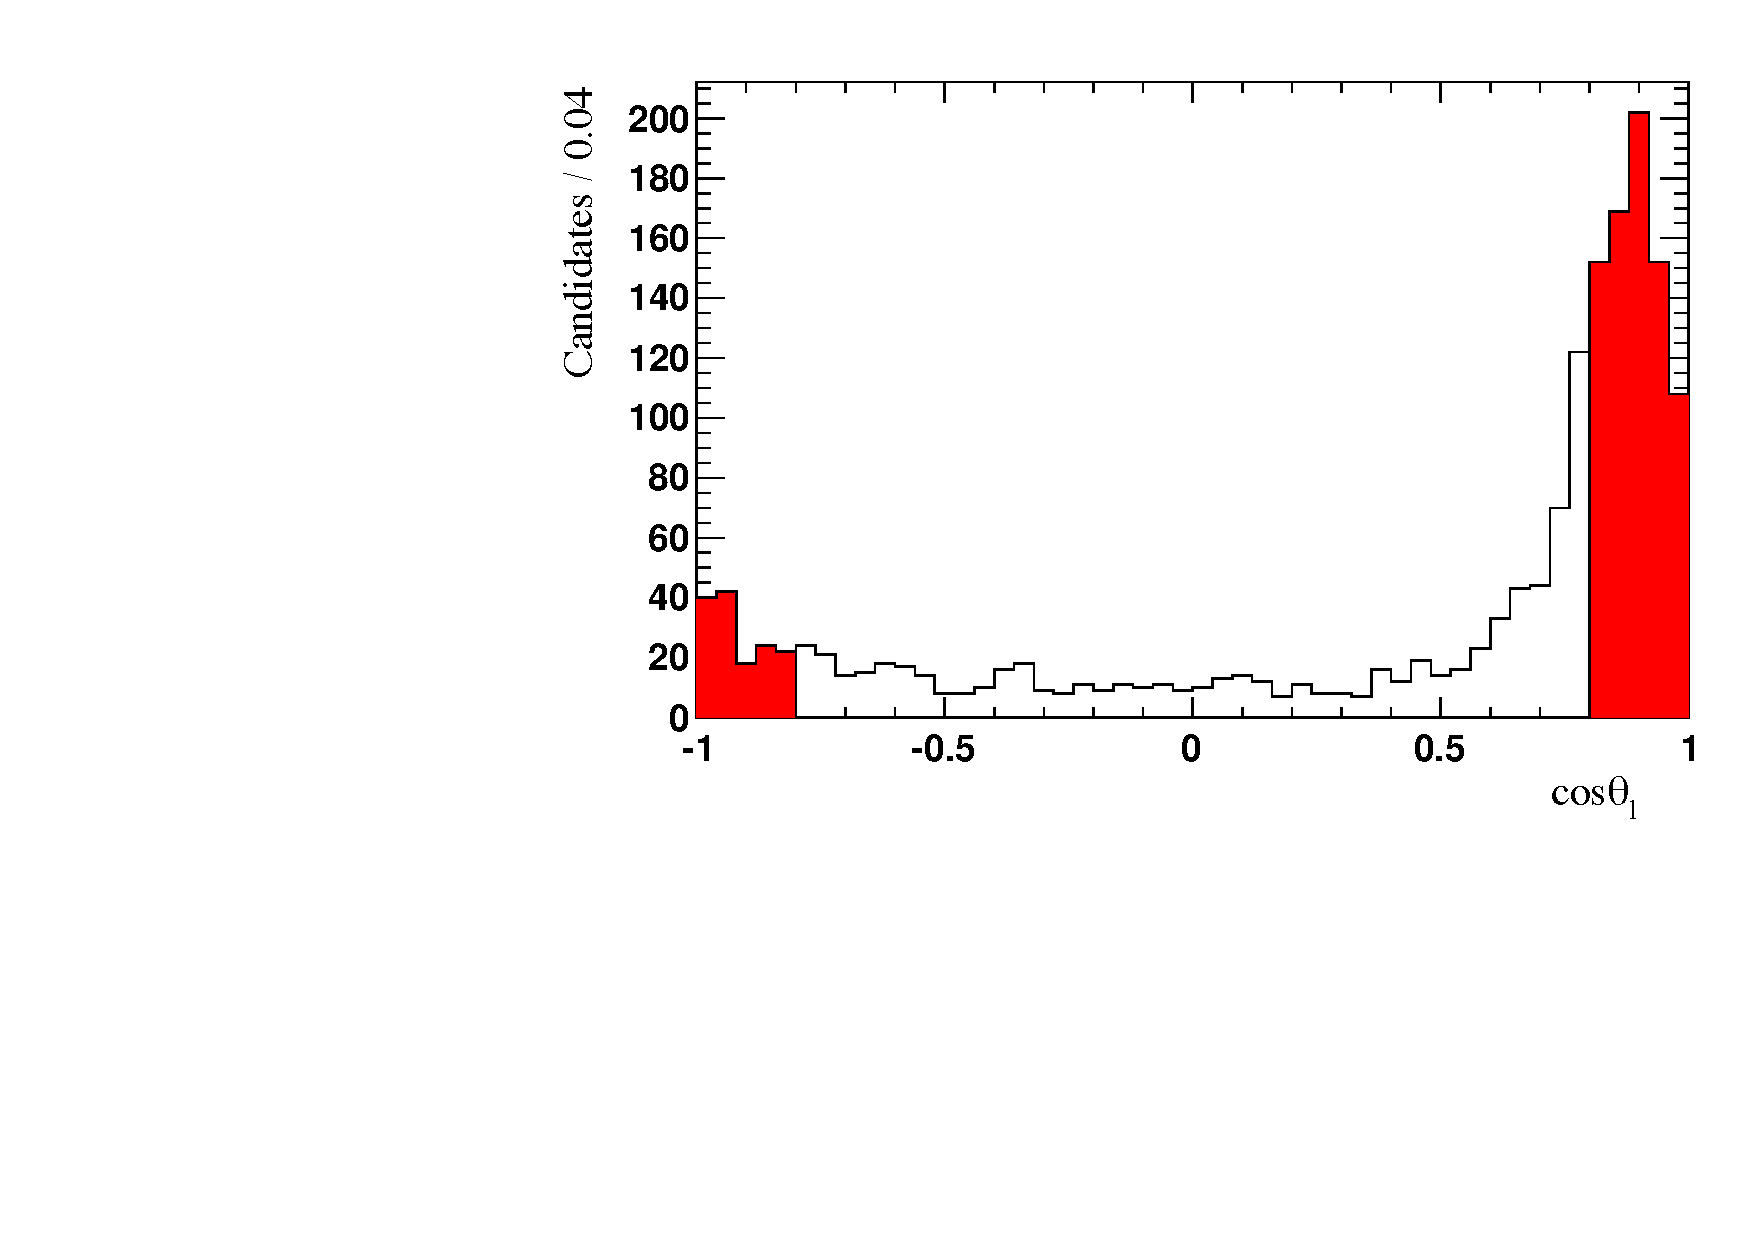
\includegraphics[width=0.49\textwidth]{RKst/figs/misreco/CosThetaL_background.pdf}
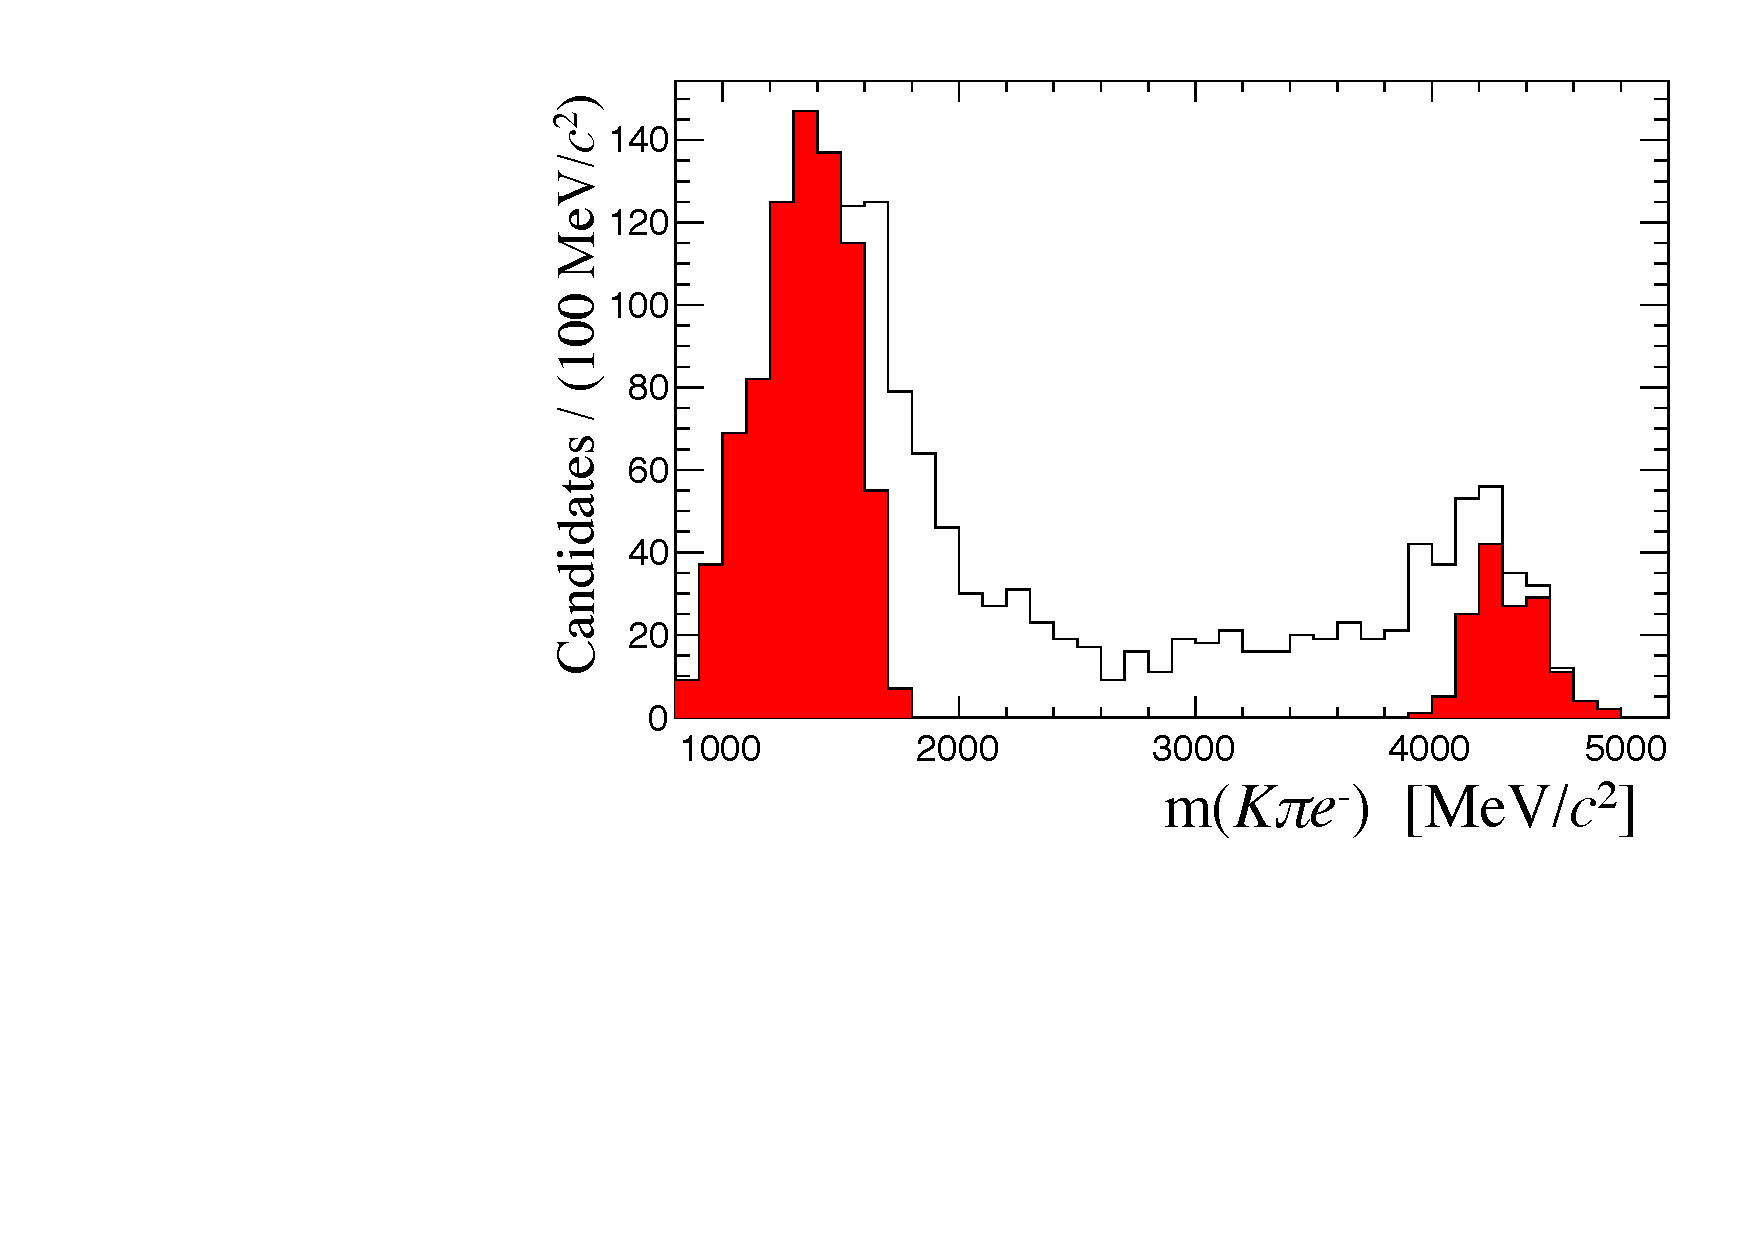
\includegraphics[width=0.49\textwidth]{RKst/figs/misreco/KstareMass_background.pdf}
\caption{Distribution of (left) $\cos \theta_\ell$ and of (right) the $m(K\pi e^-)$ invariant mass, where the \decay{\Bd}{(\Dm\to K \en \overline{\nu})\ep\nu} background is selected by requiring $m(K\pi ee) < 4800~\mevcc$. The red distribution highlights candidates with $| \cos \theta_\ell\,| > 0.8$.}
\label{fig:Denu_background}
\end{figure}

\subsubsection{\BdToKstGee}

For the low-\qsq region, a potentially dangerous background is due to the \BdToKstG decay followed by a conversion
of the photon in the detector. The branching fraction of \BdToKstG has been measured to be \mbox{\BF~= $(4.33 \pm 0.15)\times 10^{-5}$} and, 
when the photon converts into a \ee\! pair, these decays have similar characteristics to \mbox{\BdKstee}. 
In \lhcb around 40\% of photons convert before the calorimeter. Although only $\sim 10\%$ of these convert
in the VeLo and are reconstructed as long tracks, the resulting \Bd mass peaks under that of the signal, making it a dangerous background. 
This signal-like background is reduced effectively by the choice of the lower bound for the low-\qsq interval which corresponds to 
$m(ee)=20$~\mevcc. Furthermore, the \ee~pair from \BdToKstGee has a vertex at the point where the photon converts, but it may 
still be reconstructed as originating from the \Bd decay if the \ee~vertex position is determined with a large uncertainty. 
Therefore a requirement is applied on the uncertainty of the reconstructed $z$-coordinate of the \ee~pair: $\sigma_z(\ee) < 30$~mm.
%The contamination from the background is estimated in the following way: a quasi pure sample of \BdToKstGee is selected requiring that the 
%reconstructed invariant mass window for the \epem pair is smaller than 5~\mevcc. The event yield obtained on data ($881 \pm 39$ events)
%s used to rescale the prediction of the LHCb MC to get rid of problems related to an absolute prediction. 
Simulated events are used to predict the contamination from \BdToKstGee decays in the signal region which is found to be $(3.2\pm1.6)\%$.
%1.6 \%. 
%Finally as pointed out in ~\cite{LHCb-ANA-2014-009}, a conservative correction to take into account the mis-modelling 
%of the Bethe-Heitler process in Geant4 is further applied. The contamination is estimated to amount to  $(3.2\pm1.6)\%$ of the signal yield. 



\subsubsection{Other peaking backgrounds}

%A possible background could come from $\Bz \to\Kstarz\gamma$ decays where the photon converts
%into two electrons while traversing the detector. In LHCb, around 40\% of photons convert before the calorimeter,
%but only a small fraction of these, $\sim 10\%$, are reconstructed. Furthermore these events fall
%into a \qsq region well below the intervals considered in this analysis and their contribution is therefore negligible.

A potential contamination from $\Bz \to\Kstarz\eta$ and $\Bz \to\Kstarz\pi^0$, where the $\eta$ and the pion decay into
two photons, was considered and found to be small.
Furthermore, a potentially dangerous background could come from candidates where the
identity of the kaon and the pion are swapped as these candidates peak under the signal.
Although their contribution is found to be small, 0.5\%, the effect of their modelling in the fit
is taken into account when evaluating the systematic uncertainties. Finally, charmonium decays where 
the identity of the kaon, or the pion, and one of the muons  are swapped are rejected by requiring that the 
hadron-$\mu$ invariant mass \mbox{$m((h \to \mu)\mu)$}, where the muon mass hypothesis is assigned to the hadron, 
is not compatible with a \jpsi (\psitwos) resonance: $|m((h\to \mu)\mu)-m_{\jpsi, (\psitwos)} | > 60$~\mevcc.

\subsection{Partially-reconstructed background}
\label{sec:RKst_peaking_Dchains}

Partially-reconstructed candidates are defined as decays where one or more particles in the final state are not reconstructed,
resulting in $m(K\pi\ell\ell)$ values smaller than the mass of the \Bz, but with tails that can still contaminate the signal sample.
Sources of partially-reconstructed background include decays involving higher hadronic states such as 
\decay{\Bz}{(Y\to\kaon\pi X)(\jpsi\to\epem)}, where $X$ represents at least one particle that is not reconstructed. 
The $Y$ state can be a \Kstar resonance as well as \D mesons that decays semileptonically, as explained in the previous sections.
For the resonant channels, an additional source of partially-reconstructed 
background comes from decays of higher \ccbar resonances, \decay{\Bz}{(\Kstarz\to K\pi)(Y\to(\jpsi\to\epem)X)}.

To reject such backgrounds, the 4-body invariant mass $m(K\pi\ell\ell)$ is recalculated using 
\verb!DecayTreeFitter! to impose vertex constraints. For the resonant case this also includes constraining the invariant 
mass of the dilepton pair to that of the \jpsi; in this case the 4-body mass is denoted as $m(K\pi\ell\ell)_{\jpsi}$. This constraint 
pushes partially-reconstructed candidates towards low $m(K\pi\ell\ell)_{\jpsi}$ values, resulting in no contamination above 5150~\mevcc. 

This requirement is implicitly applied for the muon channels by the definition of the invariant mass fit-windows. For the electron channels,
the requirement $m(K\pi\ell\ell)_{\jpsi(\psitwos)} > 5150~\mevcc$ is explicitly applied to select the $\jpsi(ee)$ and $\psitwos(ee)$ samples.
For the electron rare decay channels the vertex constraint alone is not sufficient to remove all background and,
furthermore, to model correctly the long radiative tails of the mass shapes, a fit region that extends 
down to 4500~\mevcc~is necessary. For these reasons the requirement is not applied for the electron rare decay channels
and, as a consequence, the partially-reconstructed background is still relevant and needs to be modelled in the fit. % (for details see Sec.~\ref{sec:RKst_misreco_fit}).


%Mis-reconstructed background is defined as decays where one or more particles are not reconstructed.
%The candidates built from these decays tend to have a low 4-body invariant mass as some particles are not reconstructed.
%A source of mis-reconstructed background is due to cascade decays with a \Bz decaying semileptonically
%into a $D$ meson which also decays semileptonically, e.g. $\Bz\to D^{-} \ell^+ \bar{\nu_\ell}$
%followed by $D^{-} \to \Kstarz \ell^- \nu_\ell$. 
%This is in general true for any partially-reconstructed  background from $B$ decays.
%
%To remove this background in the muonic channels, the 4-body $m(K\pi\mumu)$ invariant mass is recalculated
%with a kinematical fit using the \verb!DecayTreeFitter! package. In the resonant case this includes a constraint of the dilepton
%mass to be the \jpsi nominal mass and in both rare and resonant cases each particles is constrained to point to 
%its origin vertex. This constraint has the effect of pushing the misreconstructed events far from the \Bz peak.
%Therefore, to avoid this background, it is sufficient to limit the analysis to 4-body invariant masses
%above 5150~\mevcc.

%In the electron case it is instead important to fit a wider mass window to correctly constrain the background
%therefore one cannot eliminate this mis-reconstructed background which is then modelled in the fit
%(for details see Sec.~\ref{sec:RKst_misreco_fit}).

\subsection{Bremsstrahlung corrected mass}
\label{sec:HOP}

For the electron channels it is particularly difficult to separate partially-reconstructed and combinatorial background from the 
long radiative tail of the signal. Additional information to reduce these backgrounds is provided by the decay kinematics: 
the transverse momenta of the \Kstarz and dielectron, defined relative to the flight direction\footnote{The flight direction is defined 
using the primary and the decay vertices.} of the parent \Bz meson, should be equal and opposite, as illustrated \mbox{in Fig.~\ref{fig:schemaHOP}}.
%\cite{LHCb-INT-2015-000}.
%In fact for the \Bz daughters, the \Kstarz and the dielectron, the momentum components orthogonal to the flight 
%direction\footnote{The flight direction is defined using the primary and the decay vertices.} of the \Bz meson, \pt, 
%should cancel out as described by the sketch shown in Fig.~\ref{fig:schemaHOP}.
\begin{figure}[b]
 \centering
    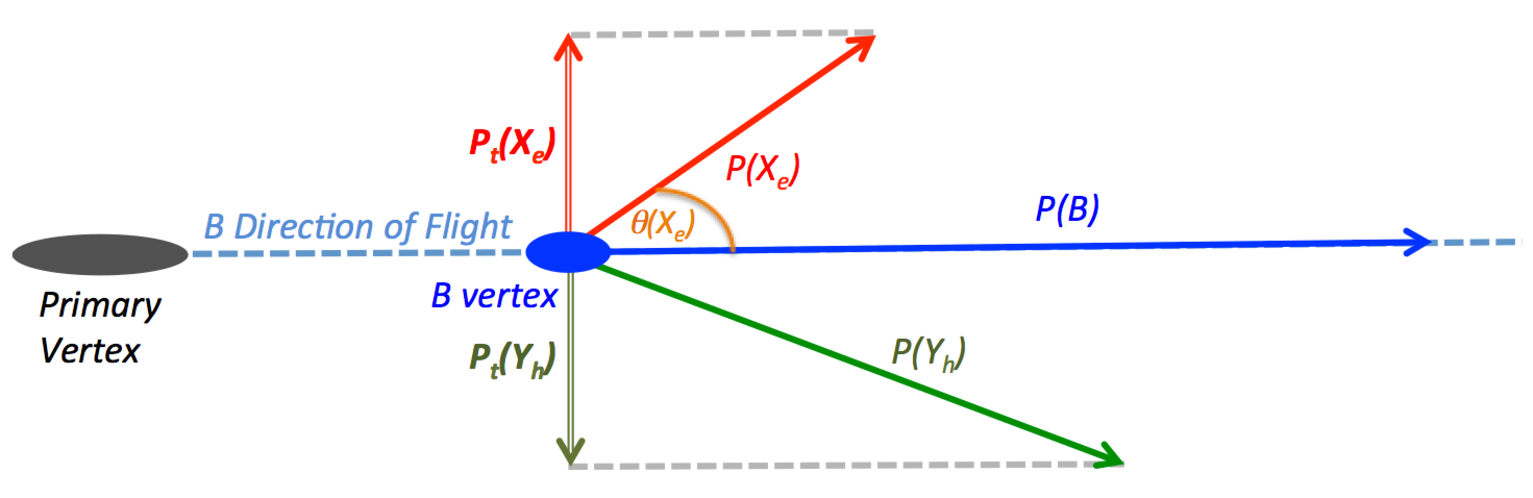
\includegraphics[width=0.9\linewidth]{RKst/figs/HOP/schemaHOP.pdf}
  \caption{ Schematic of the kinematic of a $B \to Y_h X_e$ decay, highlighting the quantities relevant for the 
  definition of the bremsstrahlung correction factor, $\alpha$.}
  \label{fig:schemaHOP}
\end{figure}

The ratio between the transverse momenta, \pt, of the \Kstarz and the dielectron pair, $\alpha = \pt(\Kstarz) / \pt(\ee)$, can be used 
to check this hypothesis. When $\alpha$ deviates from one, some energy is missing in the final state. 
For signal candidates, the missing energy is most likely carried away by bremsstrahlung photons emitted
by the electrons. Therefore, one can use $\alpha$ to correct the electron momentum as $\ptot_{\textrm{corr}}(\ee) = \alpha \cdot \ptot(\ee)$.
Since bremsstrahlung photons are predominantly emitted in the direction of the electron, the same $\alpha$ correction can
be also applied to the longitudinal component of the dielectron momentum.
In contrast, the missing particles in partially-reconstructed background candidates are not necessarily emitted in the
direction of the electrons, and therefore this correction does not work properly.
A similar argument applies to the combinatorial background. 

The corrected momenta can be used to re-calculate the invariant mass of the \Bz candidate, which in the following will be
called Bremsstrahlung Corrected Mass, \mbcm. The resolution of \mbcm depends on the quality of the vertex reconstruction
and on the \Bz lifetime, and degrades as a function of \qsq. Figure~\ref{fig:hop} shows the dependence of the \Bz $\chisq_{\rm FD}$ 
(flight distance $\chisq$) as a function of \mbcm in the \qsq regions considered for the rare decay. 

As the correction factor is not meaningful for backgrounds this leads the candidates to spread out making \mbcm 
a discriminating variable between signal and background. A two-dimensional cut is adopted:
$$\mbcm > a_{\rm BCM} + b_{\rm BCM} \cdot \log(\chisq_{\rm FD}),$$
where the $a_{\rm BCM}$ and $b_{\rm BCM}$ coefficients are optimised as described in Sec.~\ref{sec:optimisation}.
%
The requirement is not applied either at high-\qsq, because the variable loses discriminating power, or to the muon 
channels for which the bremsstrahlung radiation is negligible.

%Figure~\ref{fig:hop2} shows the dependence of \mKpiee as a function of \mbcm in the considered \qsq regions. 

%The efficiency of the cut in the different bins of \qsq and for the different signal and background components is shown
%in Fig.~\ref{}. The cut efficiency is almost flat for the signal while it's rejection power is higher for low $B$ mass. 

%It should be noted that \mbcm has also a dependence on \qsq, as for high-\qsq the transverse momentum of the \Kstar, and consequently \hop, is less precisely determined.
%As a consequence, the cut turns out to be inefficient for the high-\qsq bin, where therefore it is not applied.
%No \hop requirement is used for the muon channels for which the bremsstrahlung is negligible. 

\begin{figure}[t!]
\centering
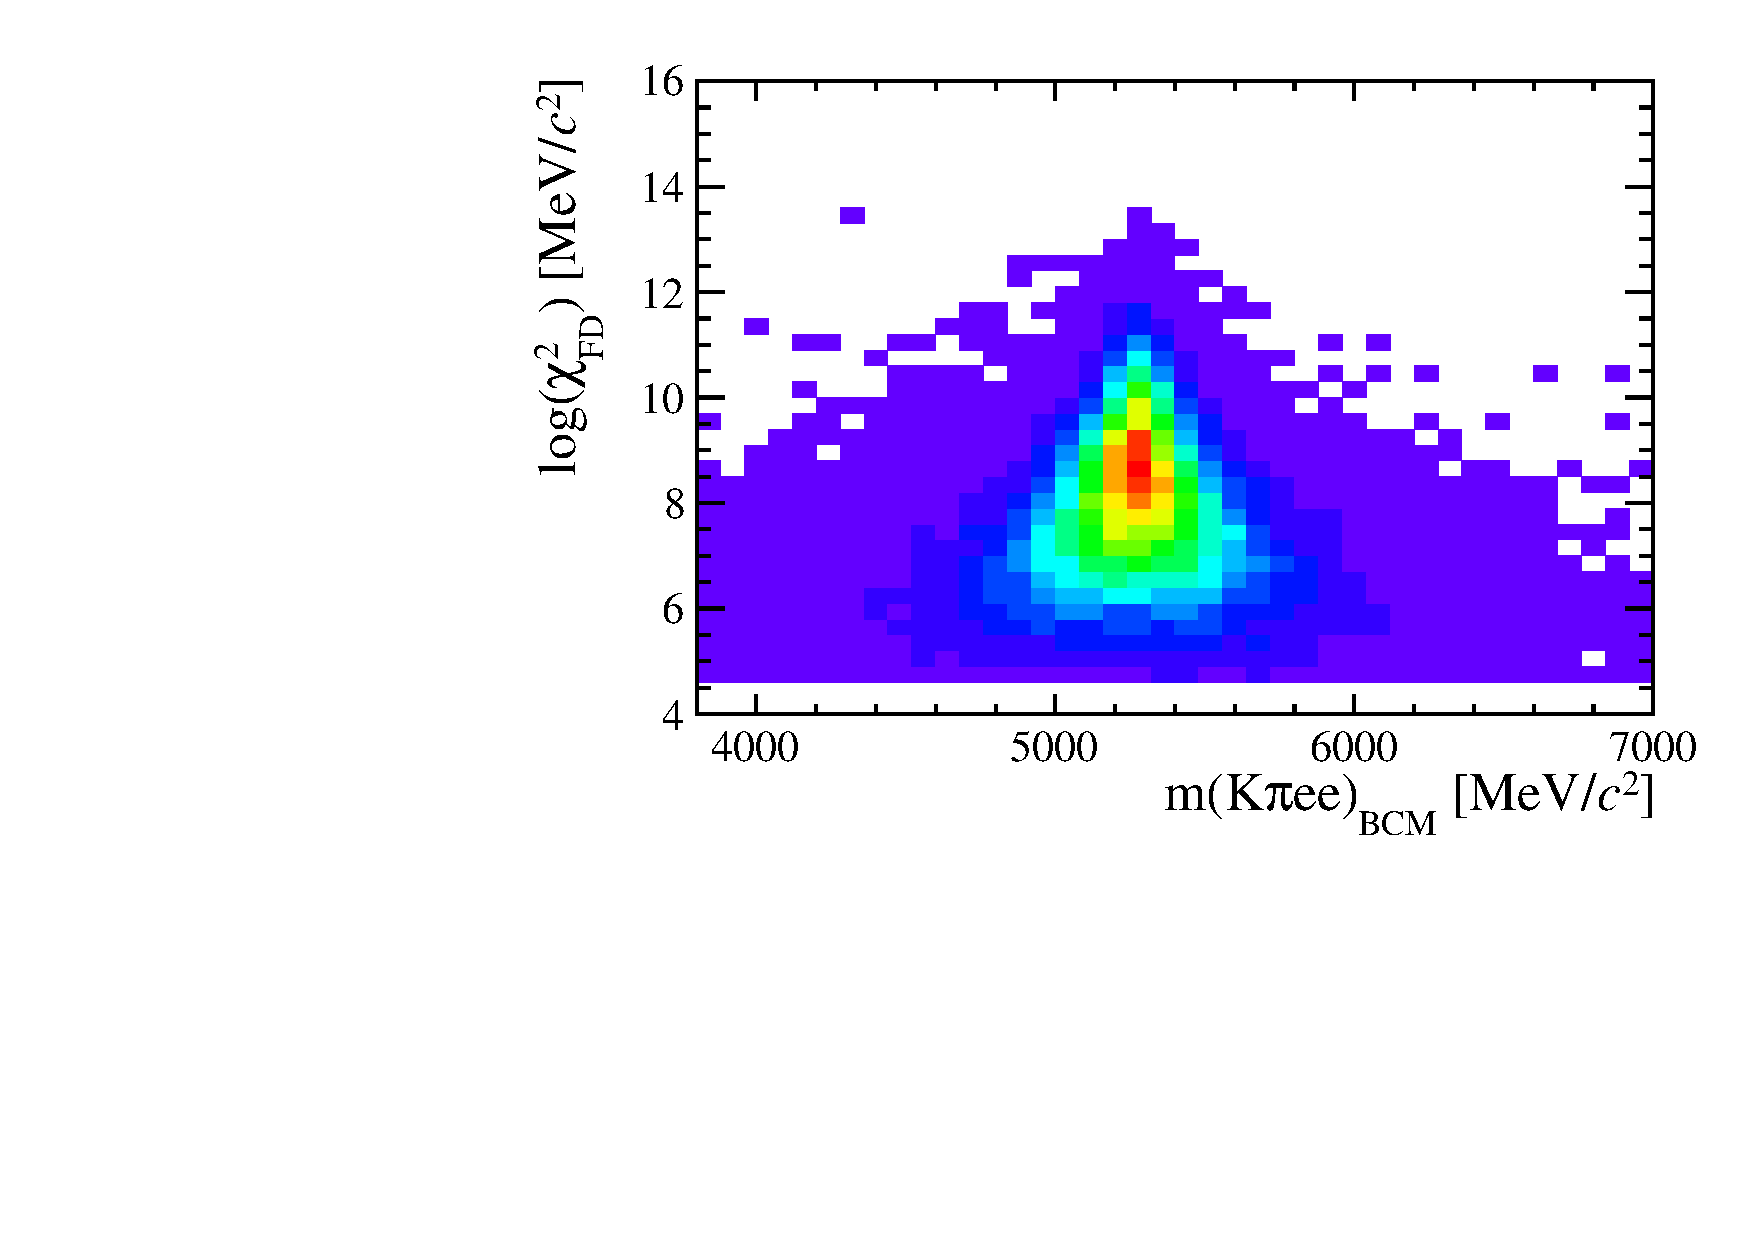
\includegraphics[width=0.49\textwidth]{RKst/figs/HOP/HOP_sig_low.pdf}
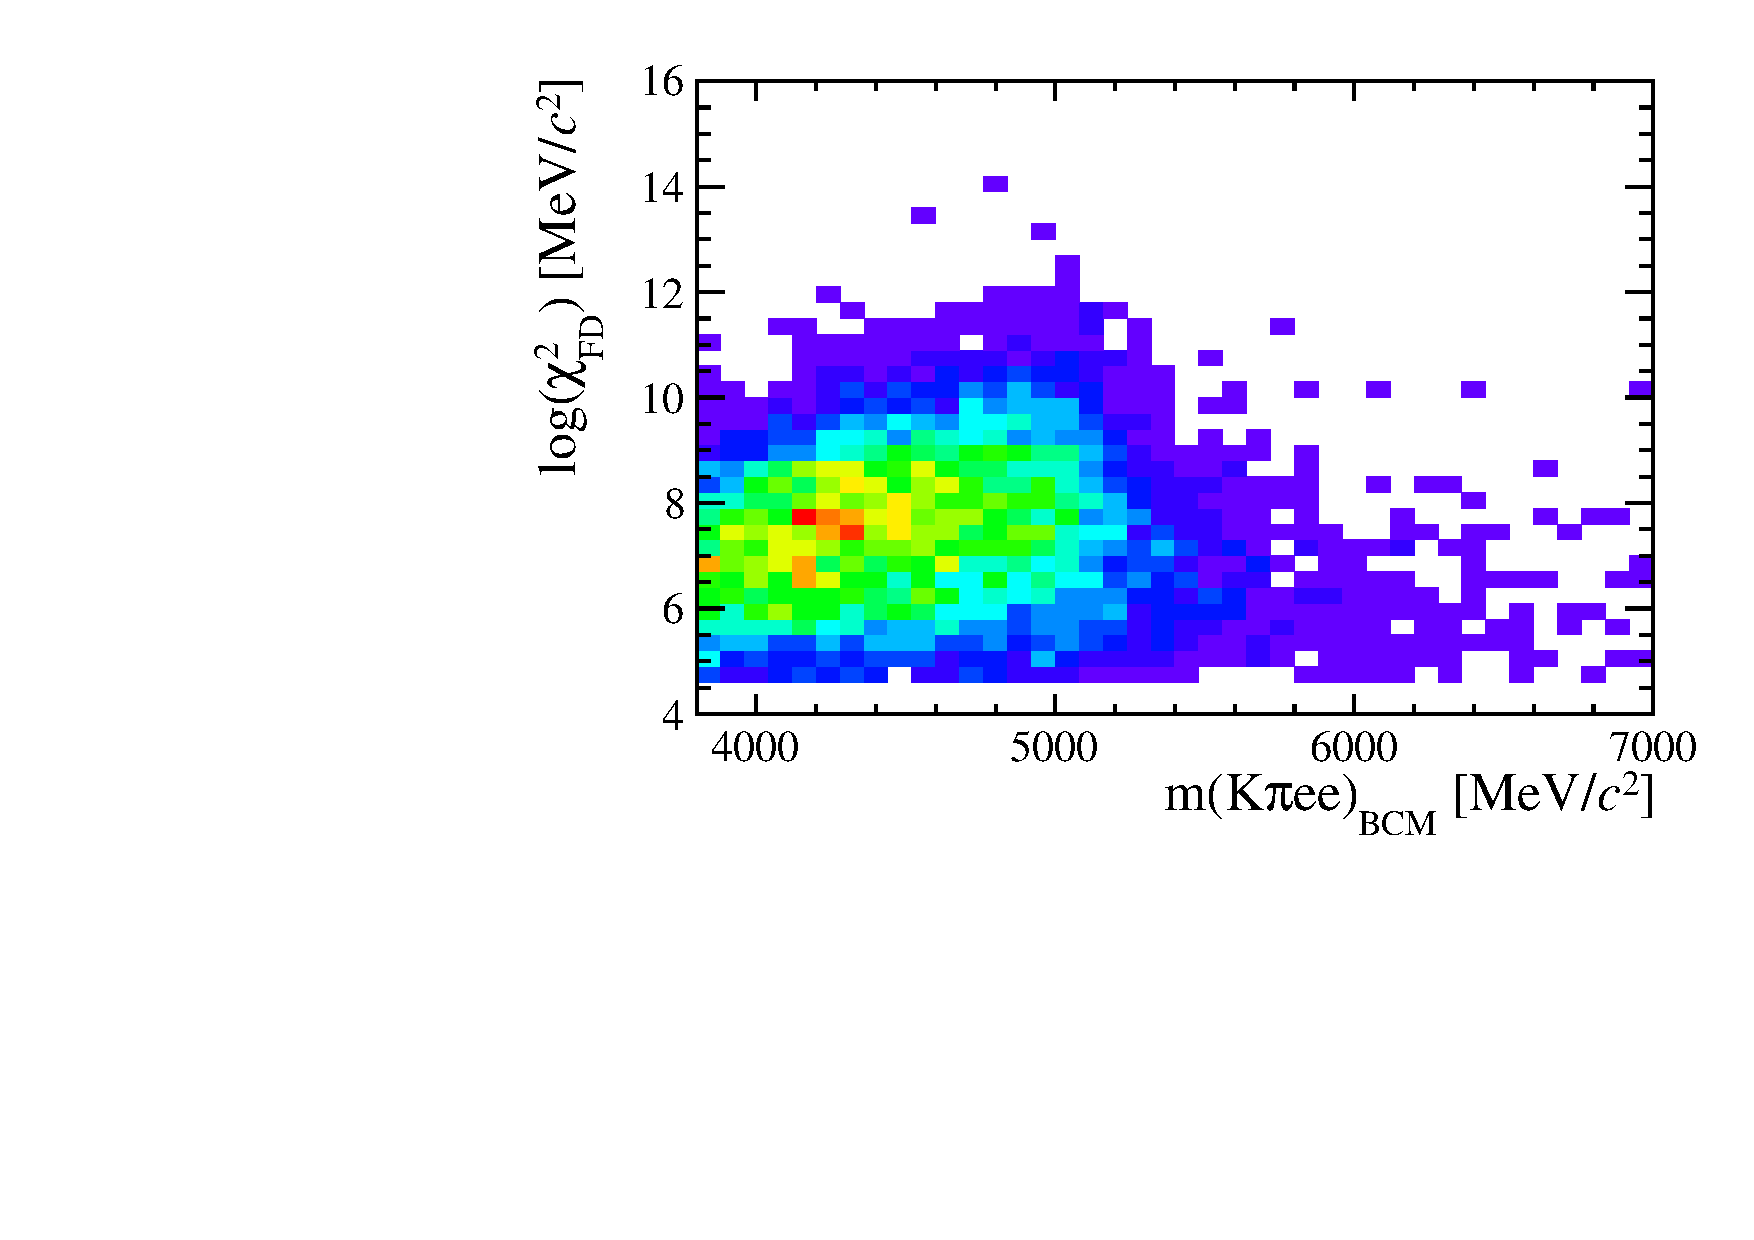
\includegraphics[width=0.49\textwidth]{RKst/figs/HOP/HOP_bkg_low.pdf}
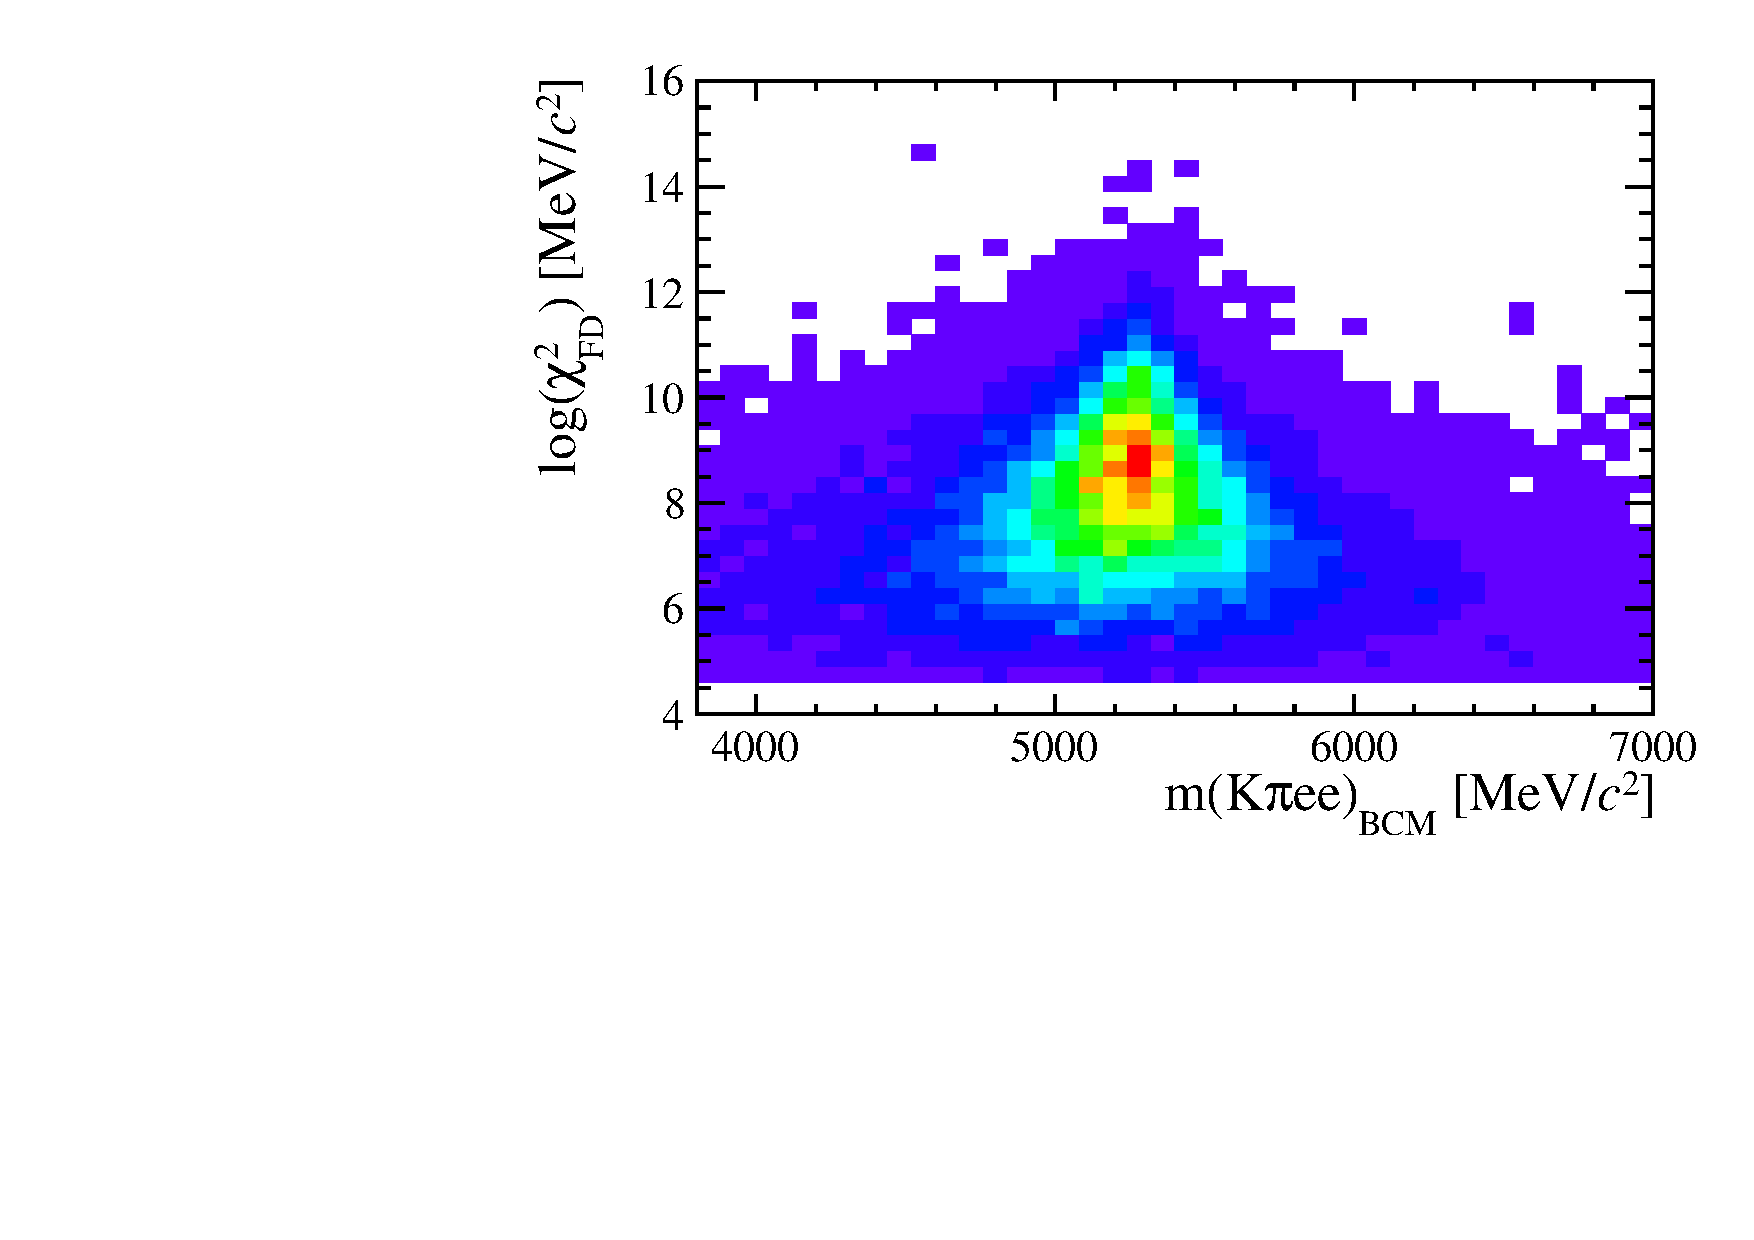
\includegraphics[width=0.49\textwidth]{RKst/figs/HOP/HOP_sig_central.pdf}
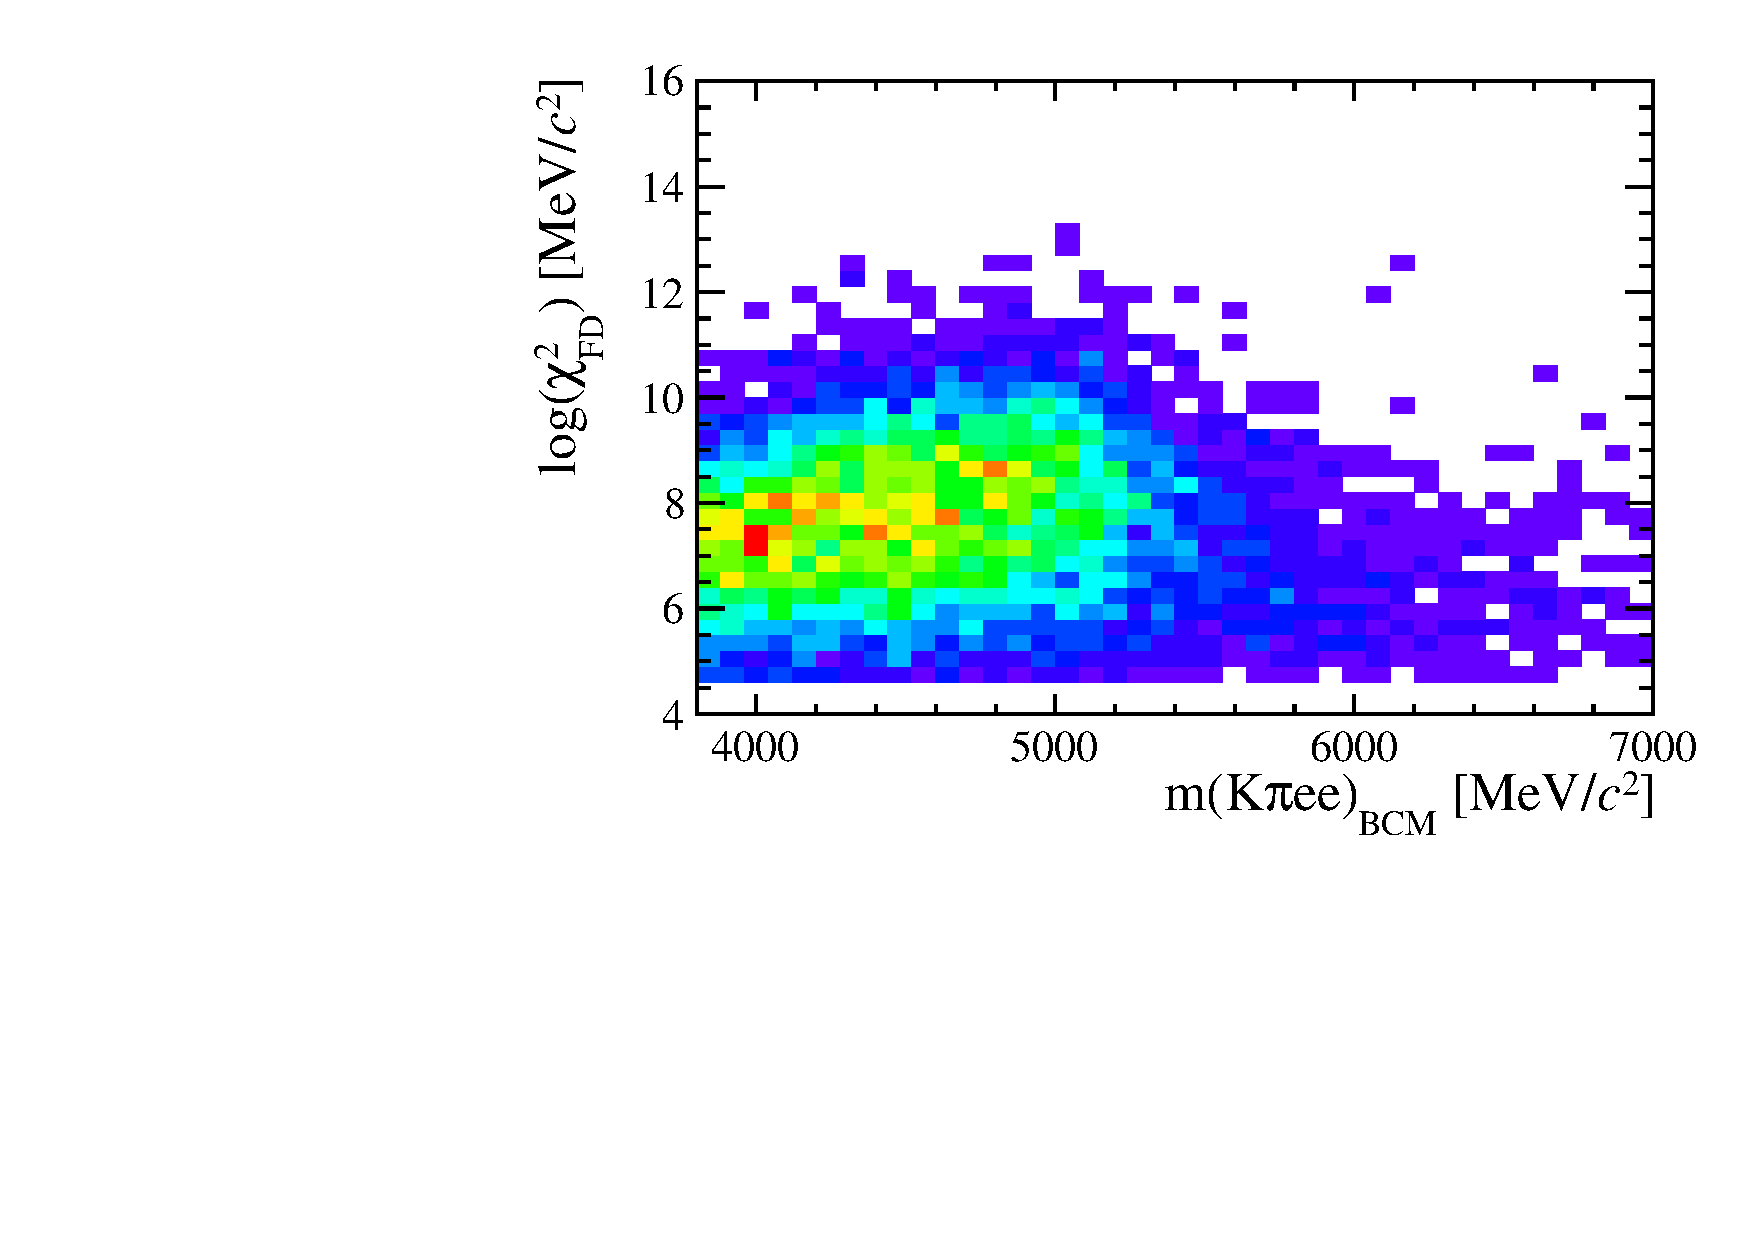
\includegraphics[width=0.49\textwidth]{RKst/figs/HOP/HOP_bkg_central.pdf}
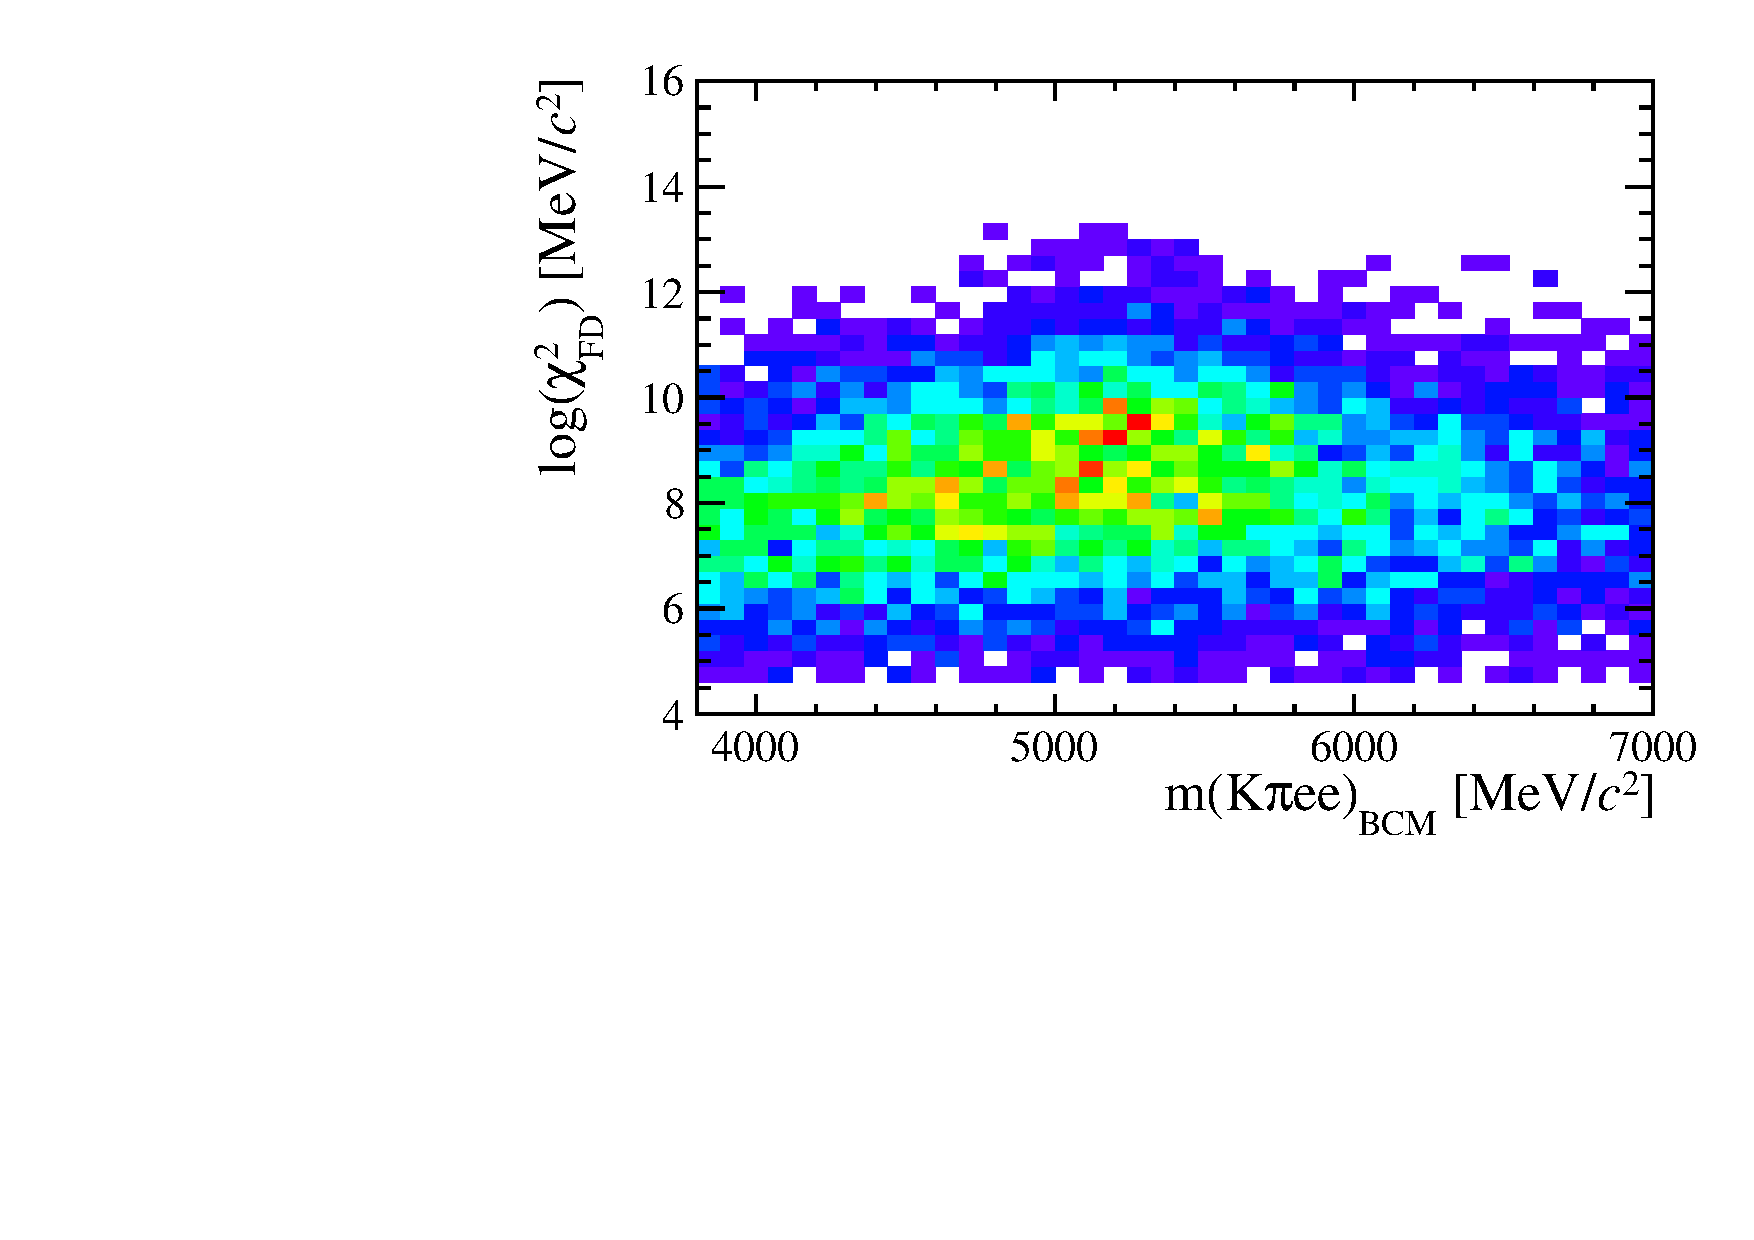
\includegraphics[width=0.49\textwidth]{RKst/figs/HOP/HOP_sig_high.pdf}
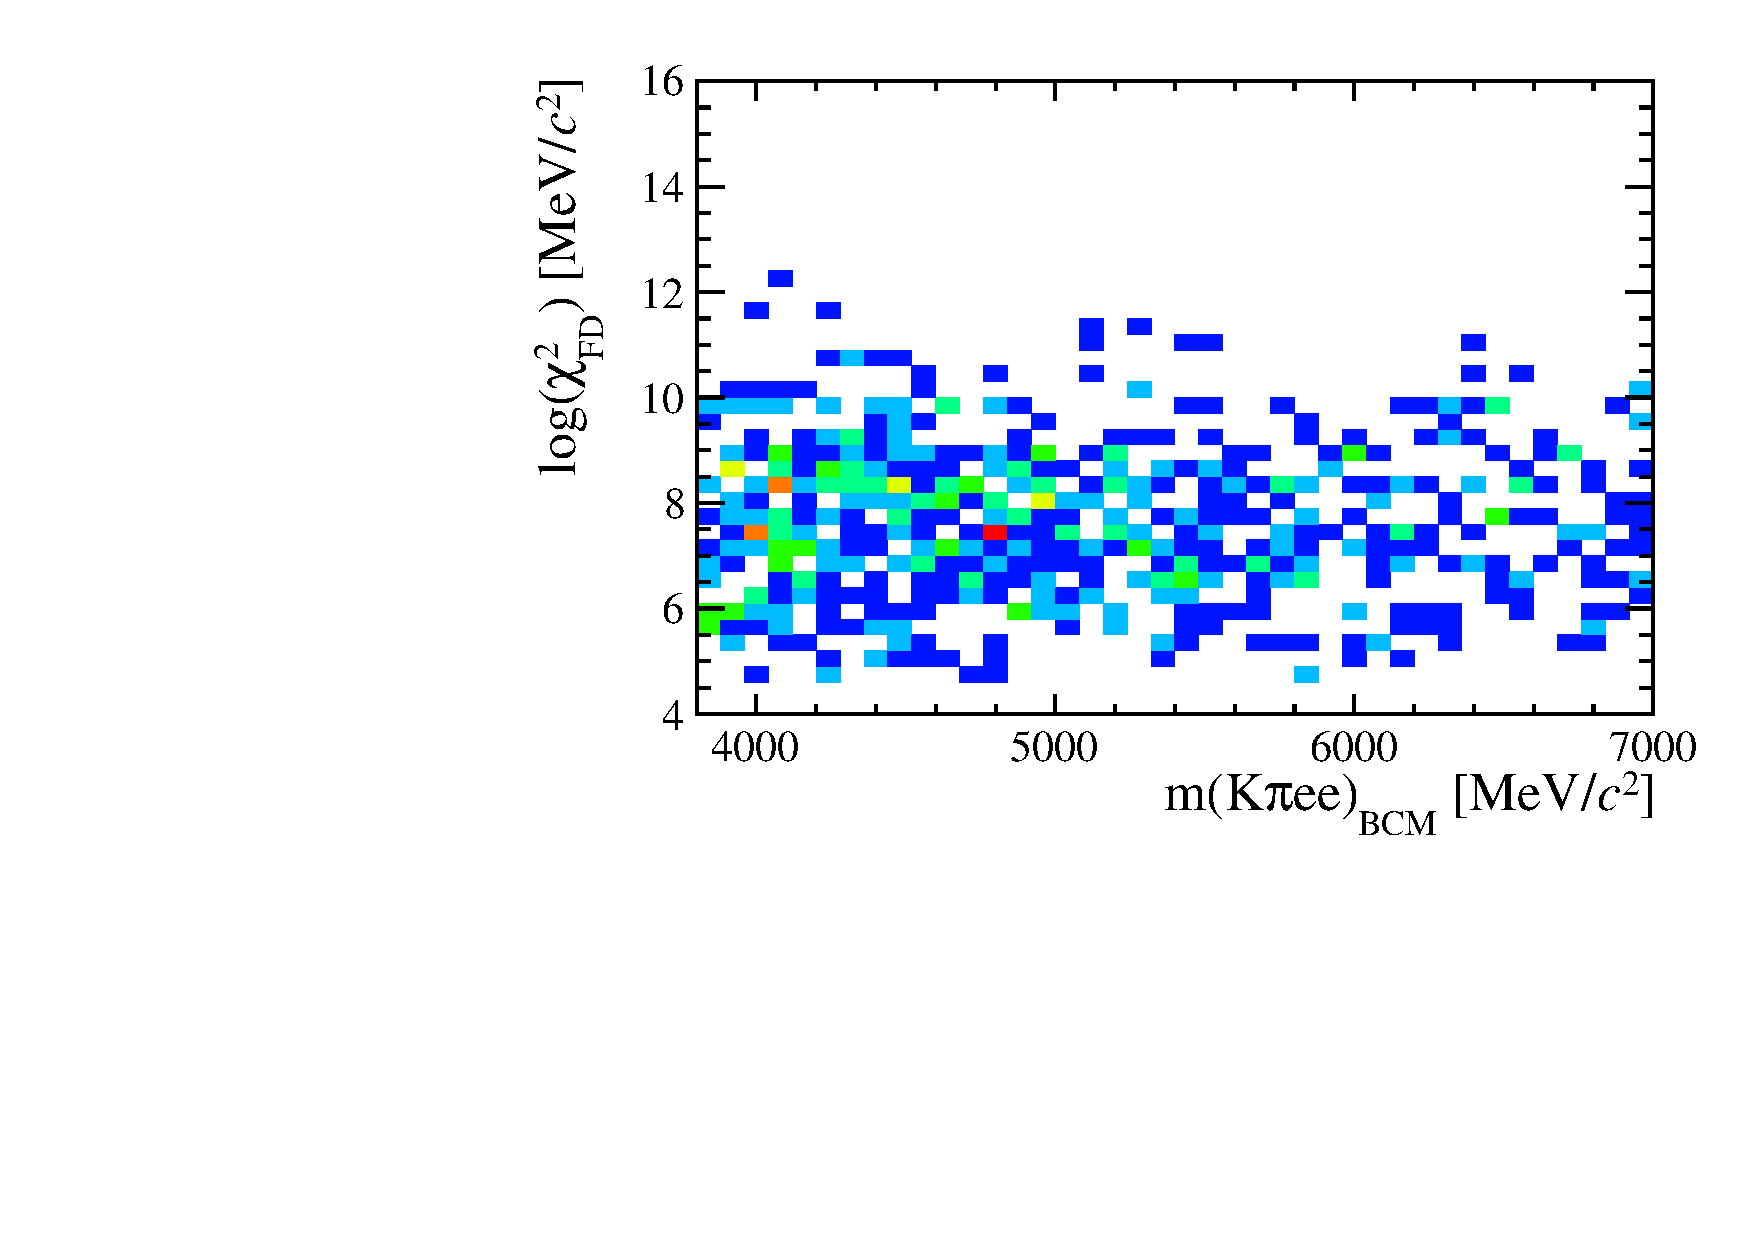
\includegraphics[width=0.49\textwidth]{RKst/figs/HOP/HOP_bkg_high.pdf}
\caption{Two-dimensional distributions of $\log(\chisq_{\rm FD})$ versus \mbcm for (left) 
\mbox{\BdToKstee} signal and (right) partially-reconstructed background.
From top to bottom the low-, central- and high-\qsq intervals.}
\label{fig:hop}

%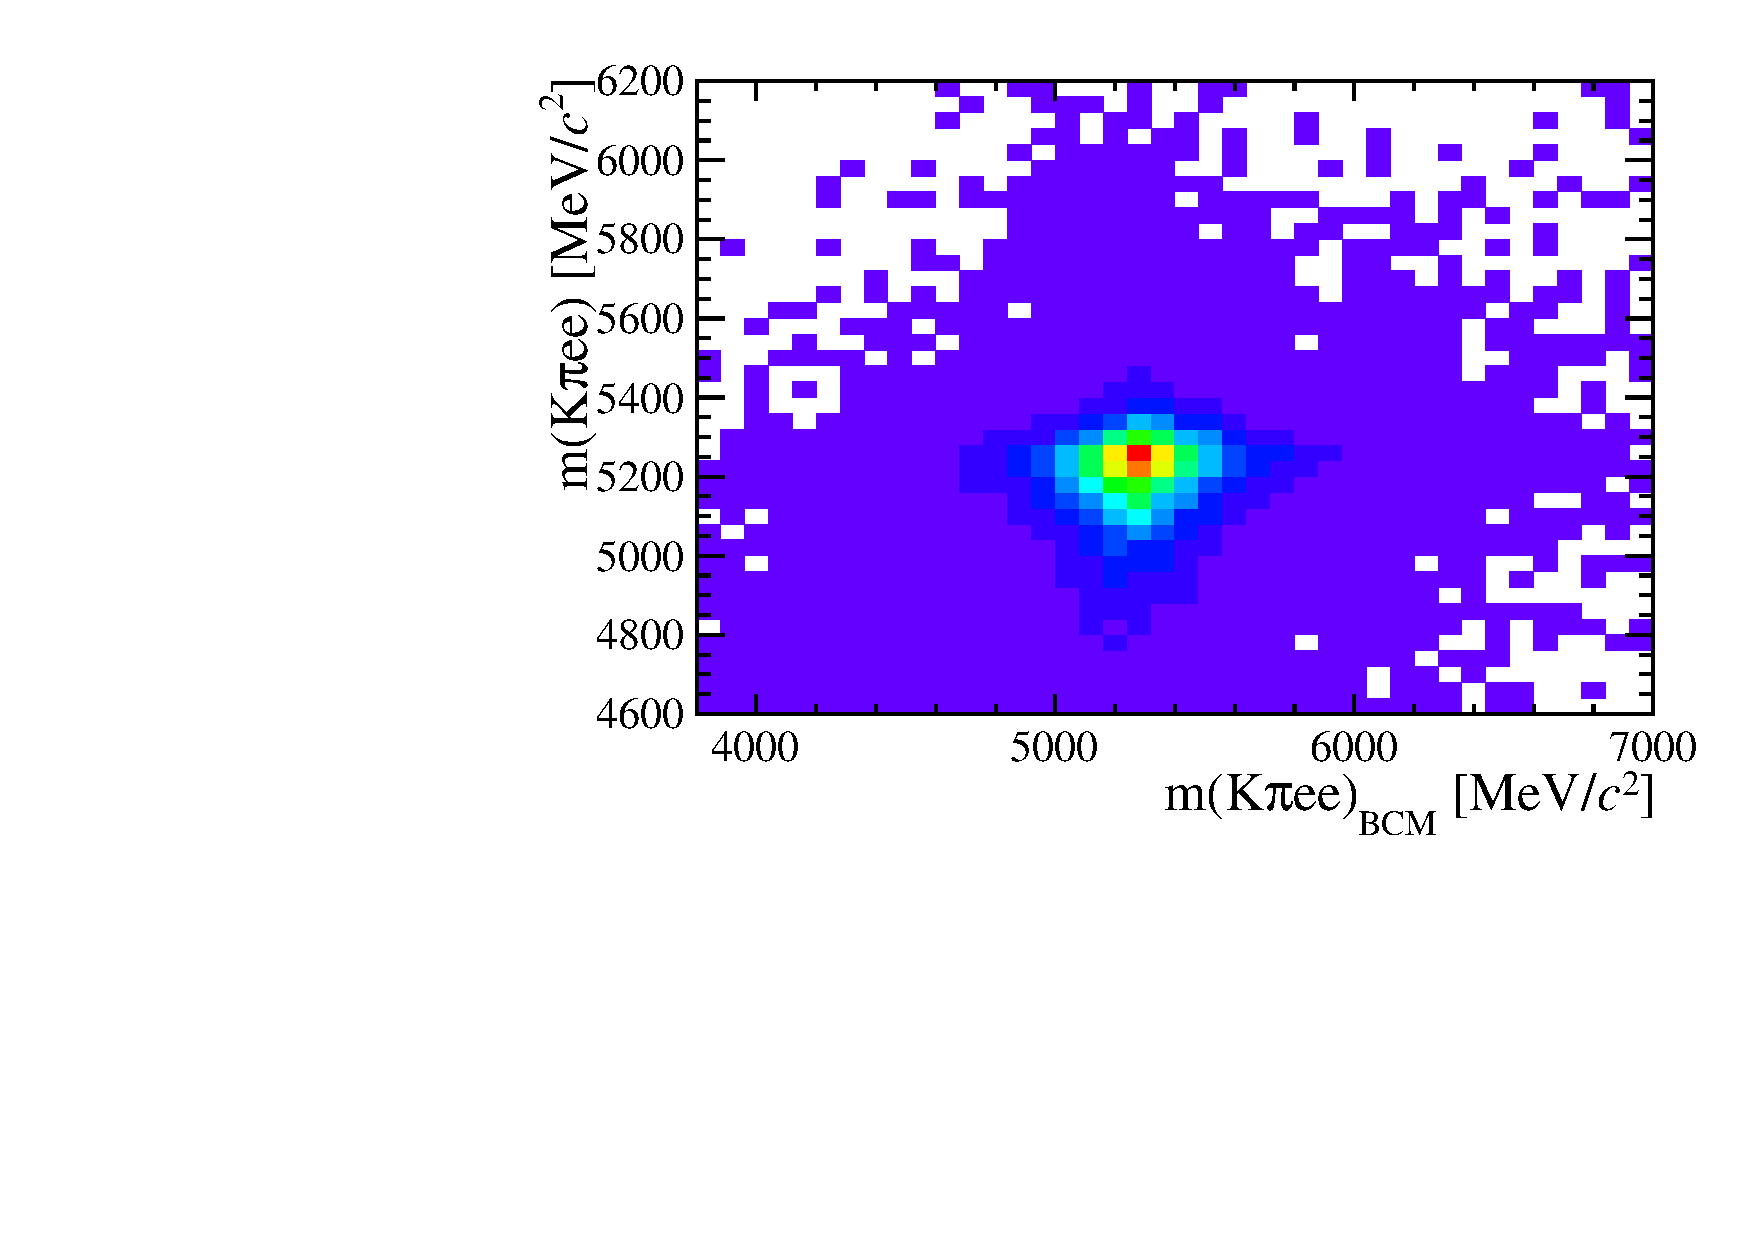
\includegraphics[width=0.48\textwidth]{RKst/figs/HOP/HOPvsM_sig_low.pdf}
%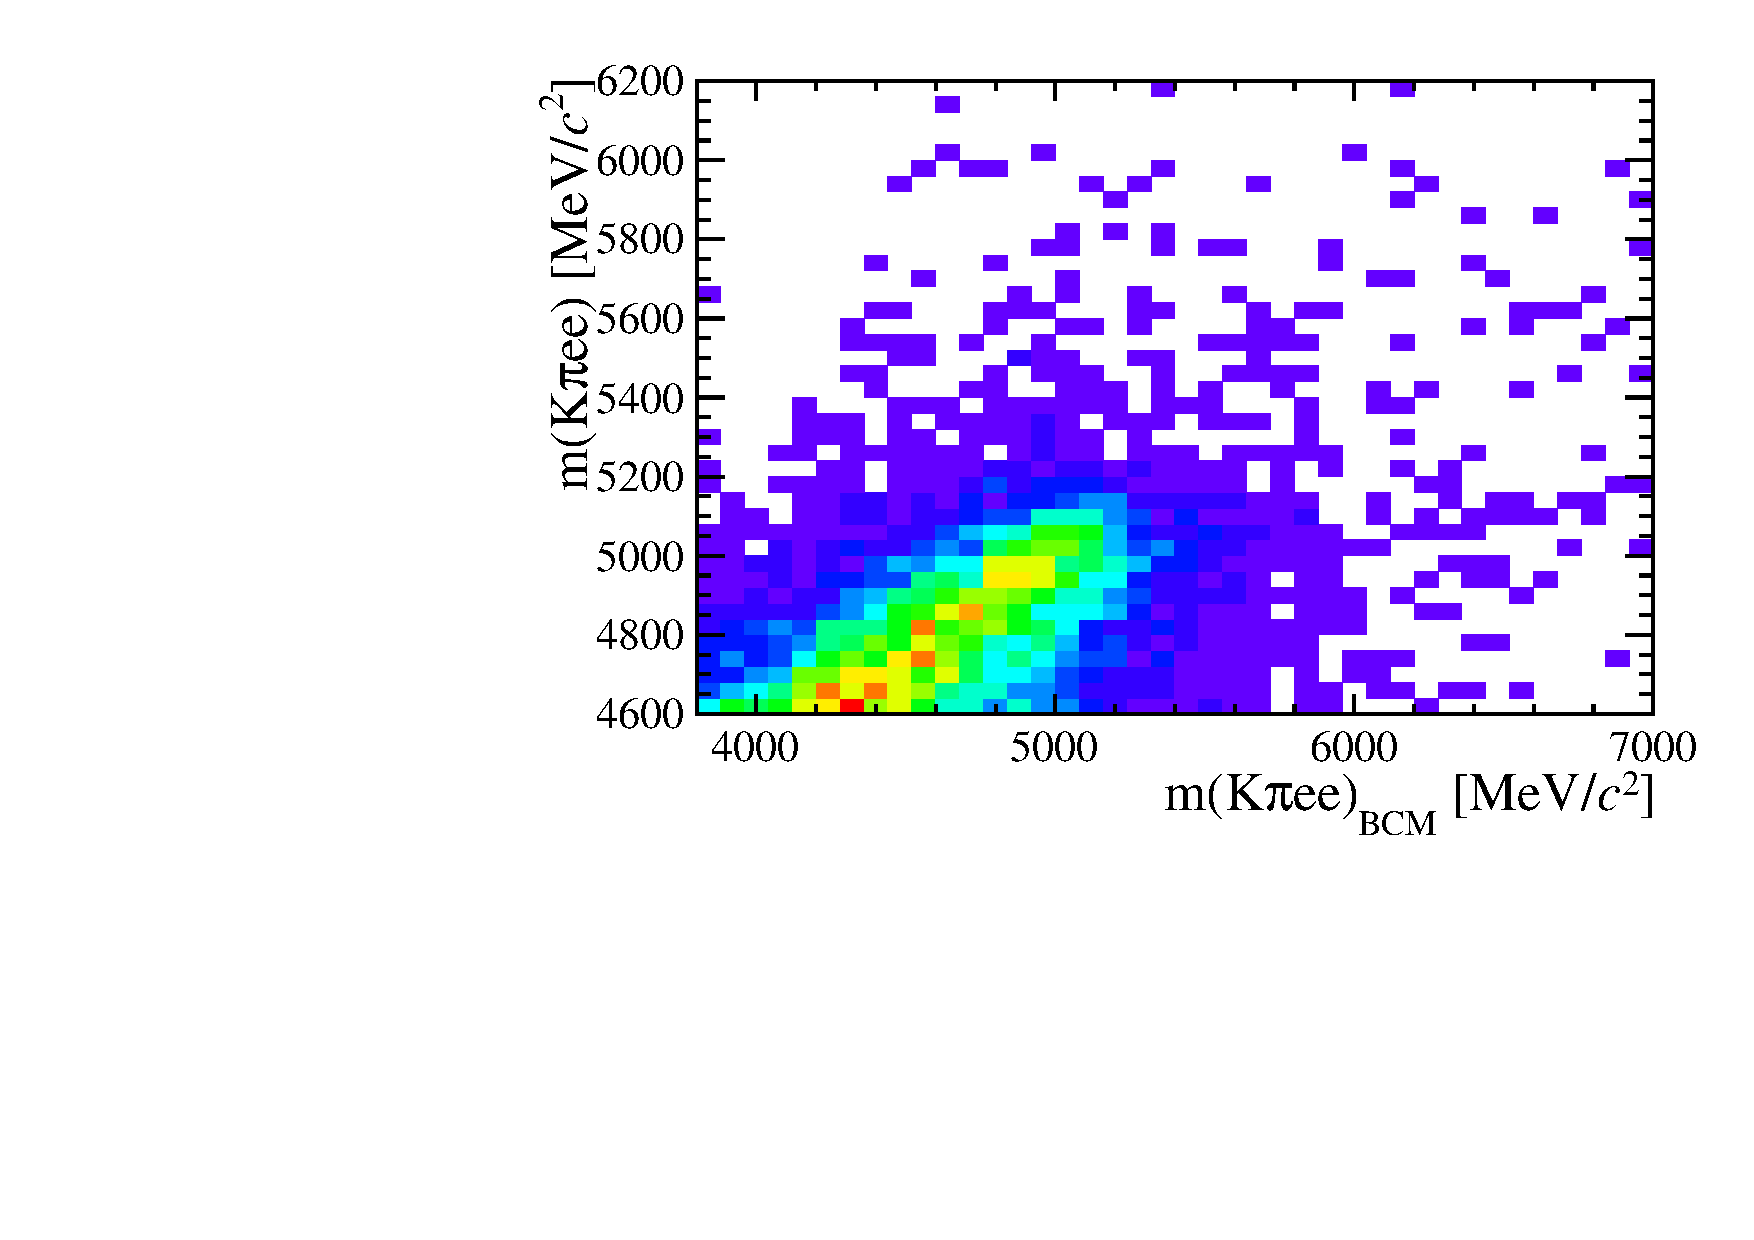
\includegraphics[width=0.48\textwidth]{RKst/figs/HOP/HOPvsM_bkg_low.pdf}
%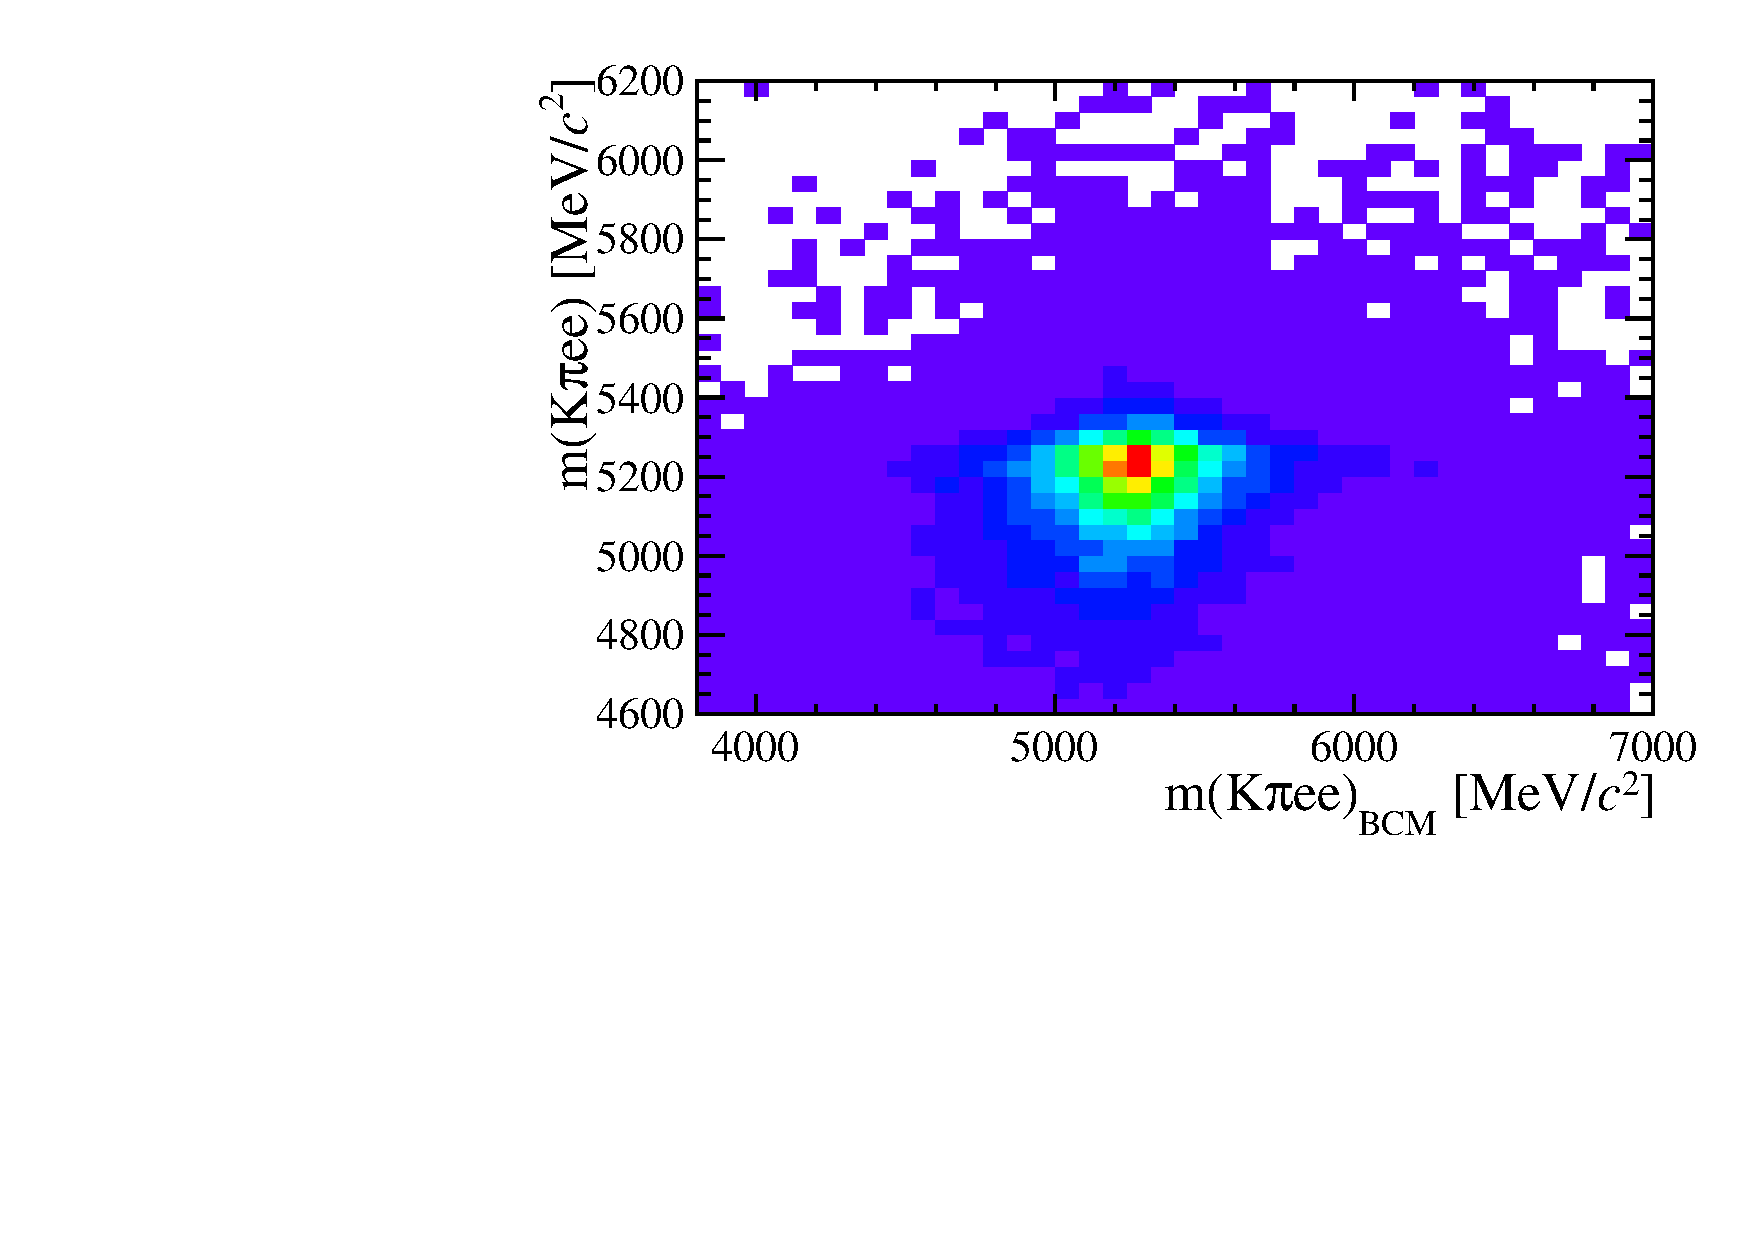
\includegraphics[width=0.48\textwidth]{RKst/figs/HOP/HOPvsM_sig_central.pdf}
%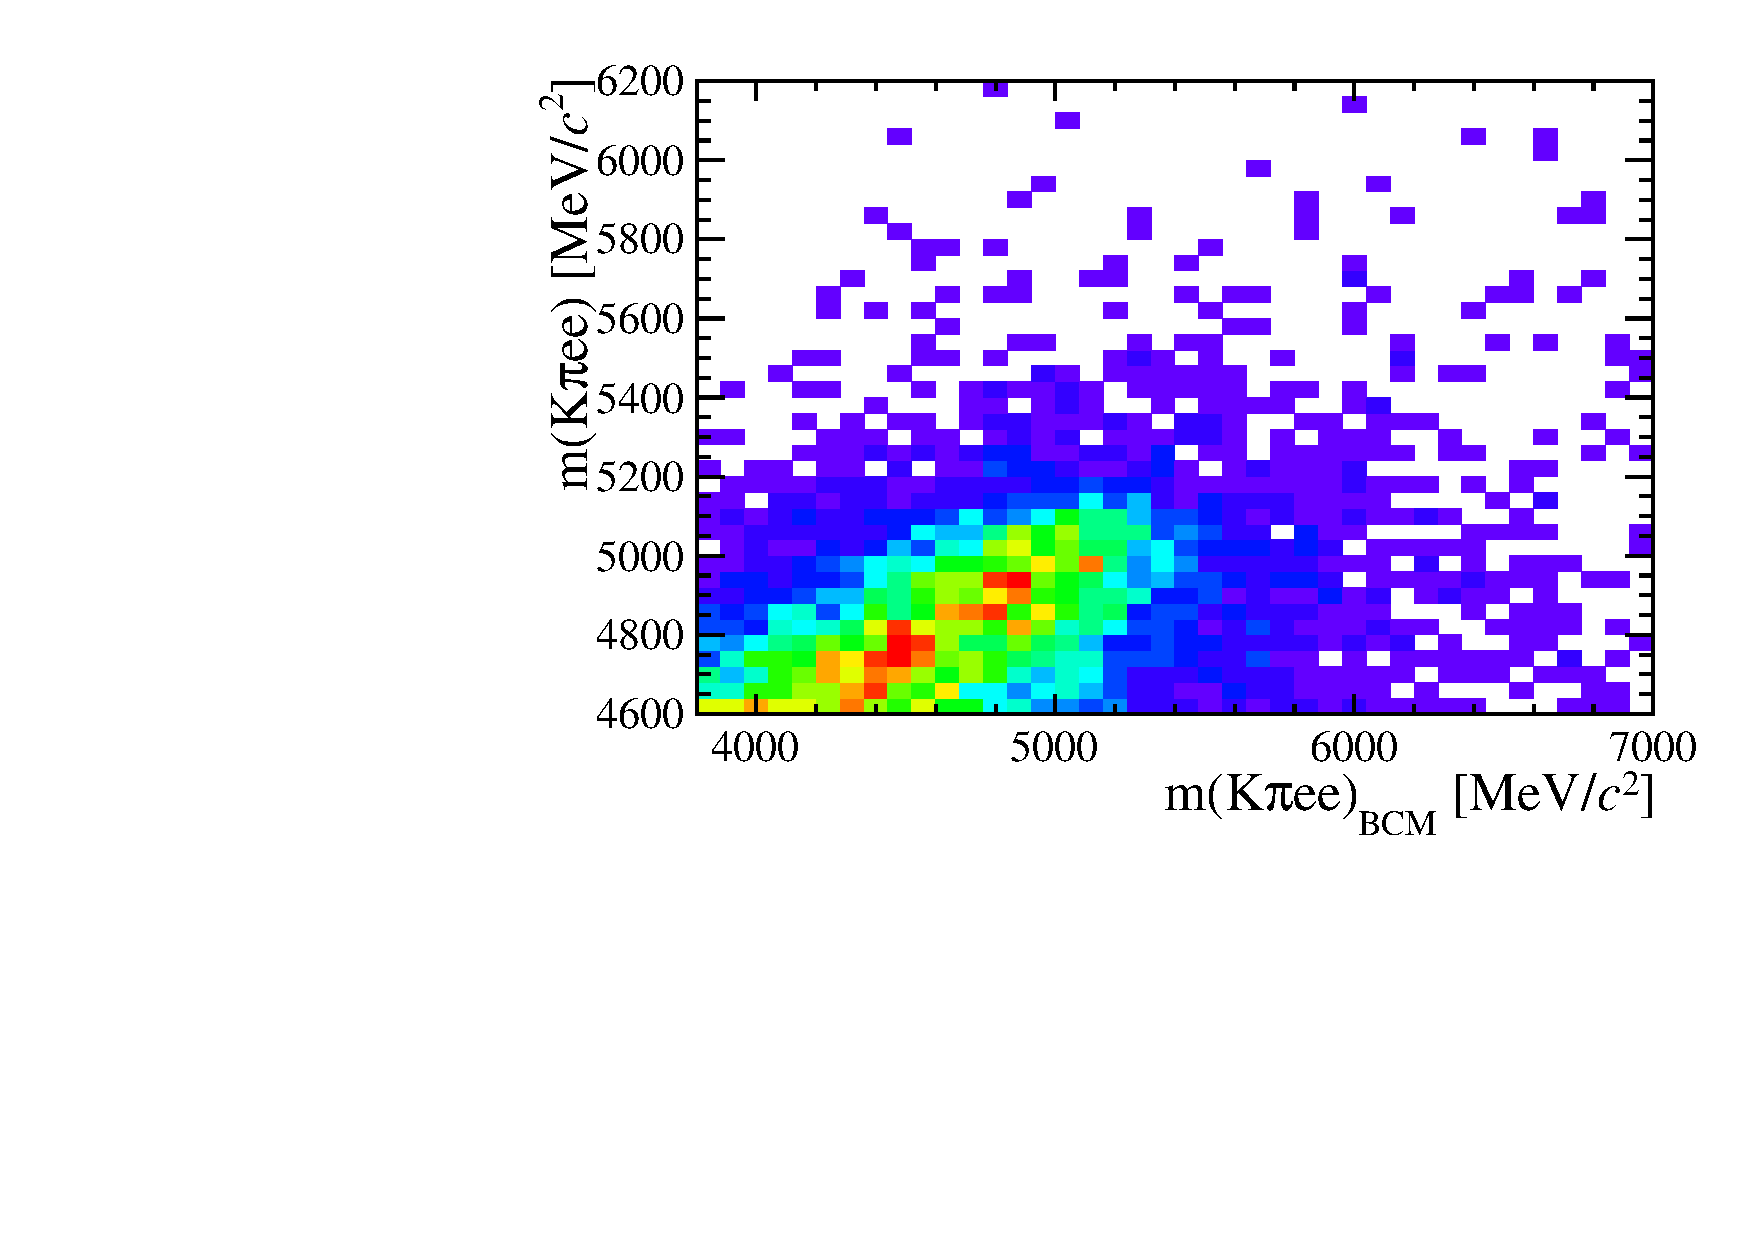
\includegraphics[width=0.48\textwidth]{RKst/figs/HOP/HOPvsM_bkg_central.pdf}
%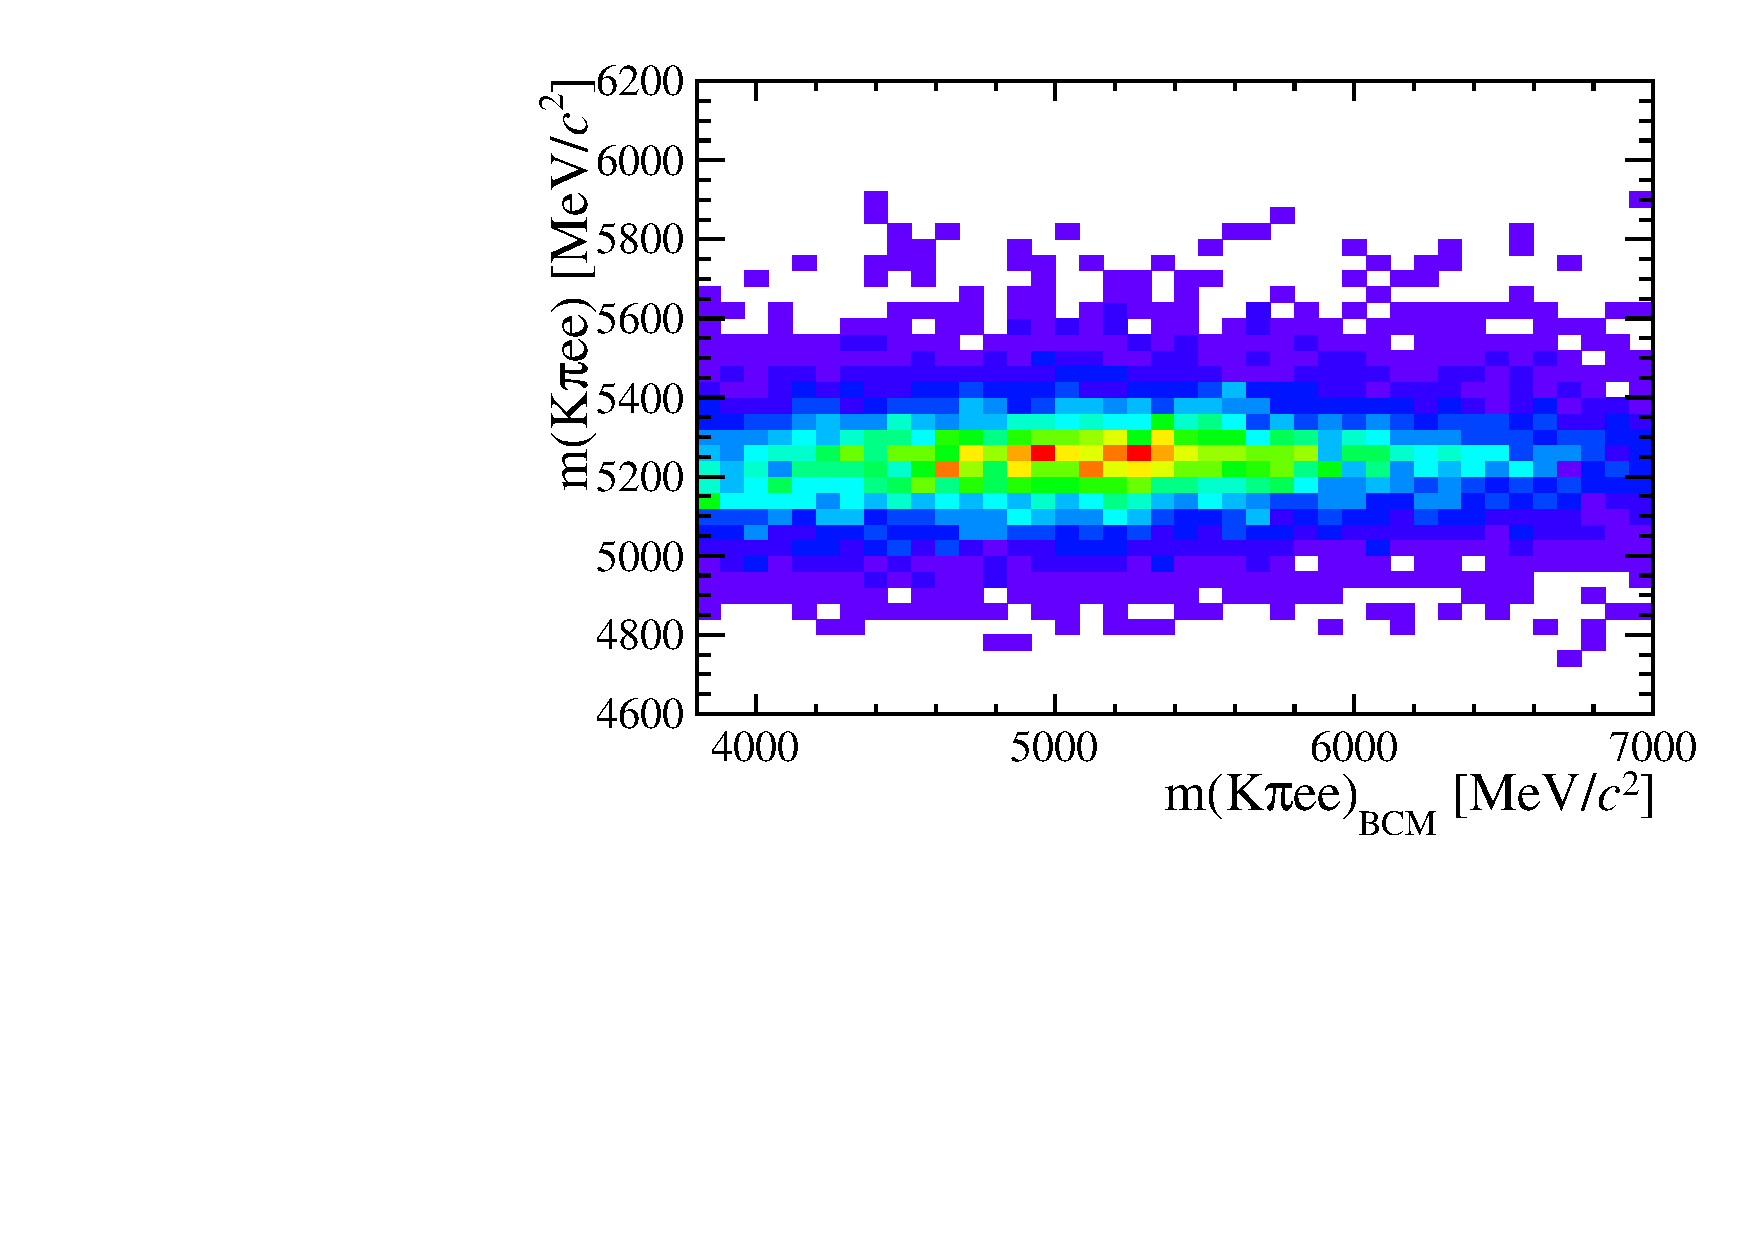
\includegraphics[width=0.48\textwidth]{RKst/figs/HOP/HOPvsM_sig_high.pdf}
%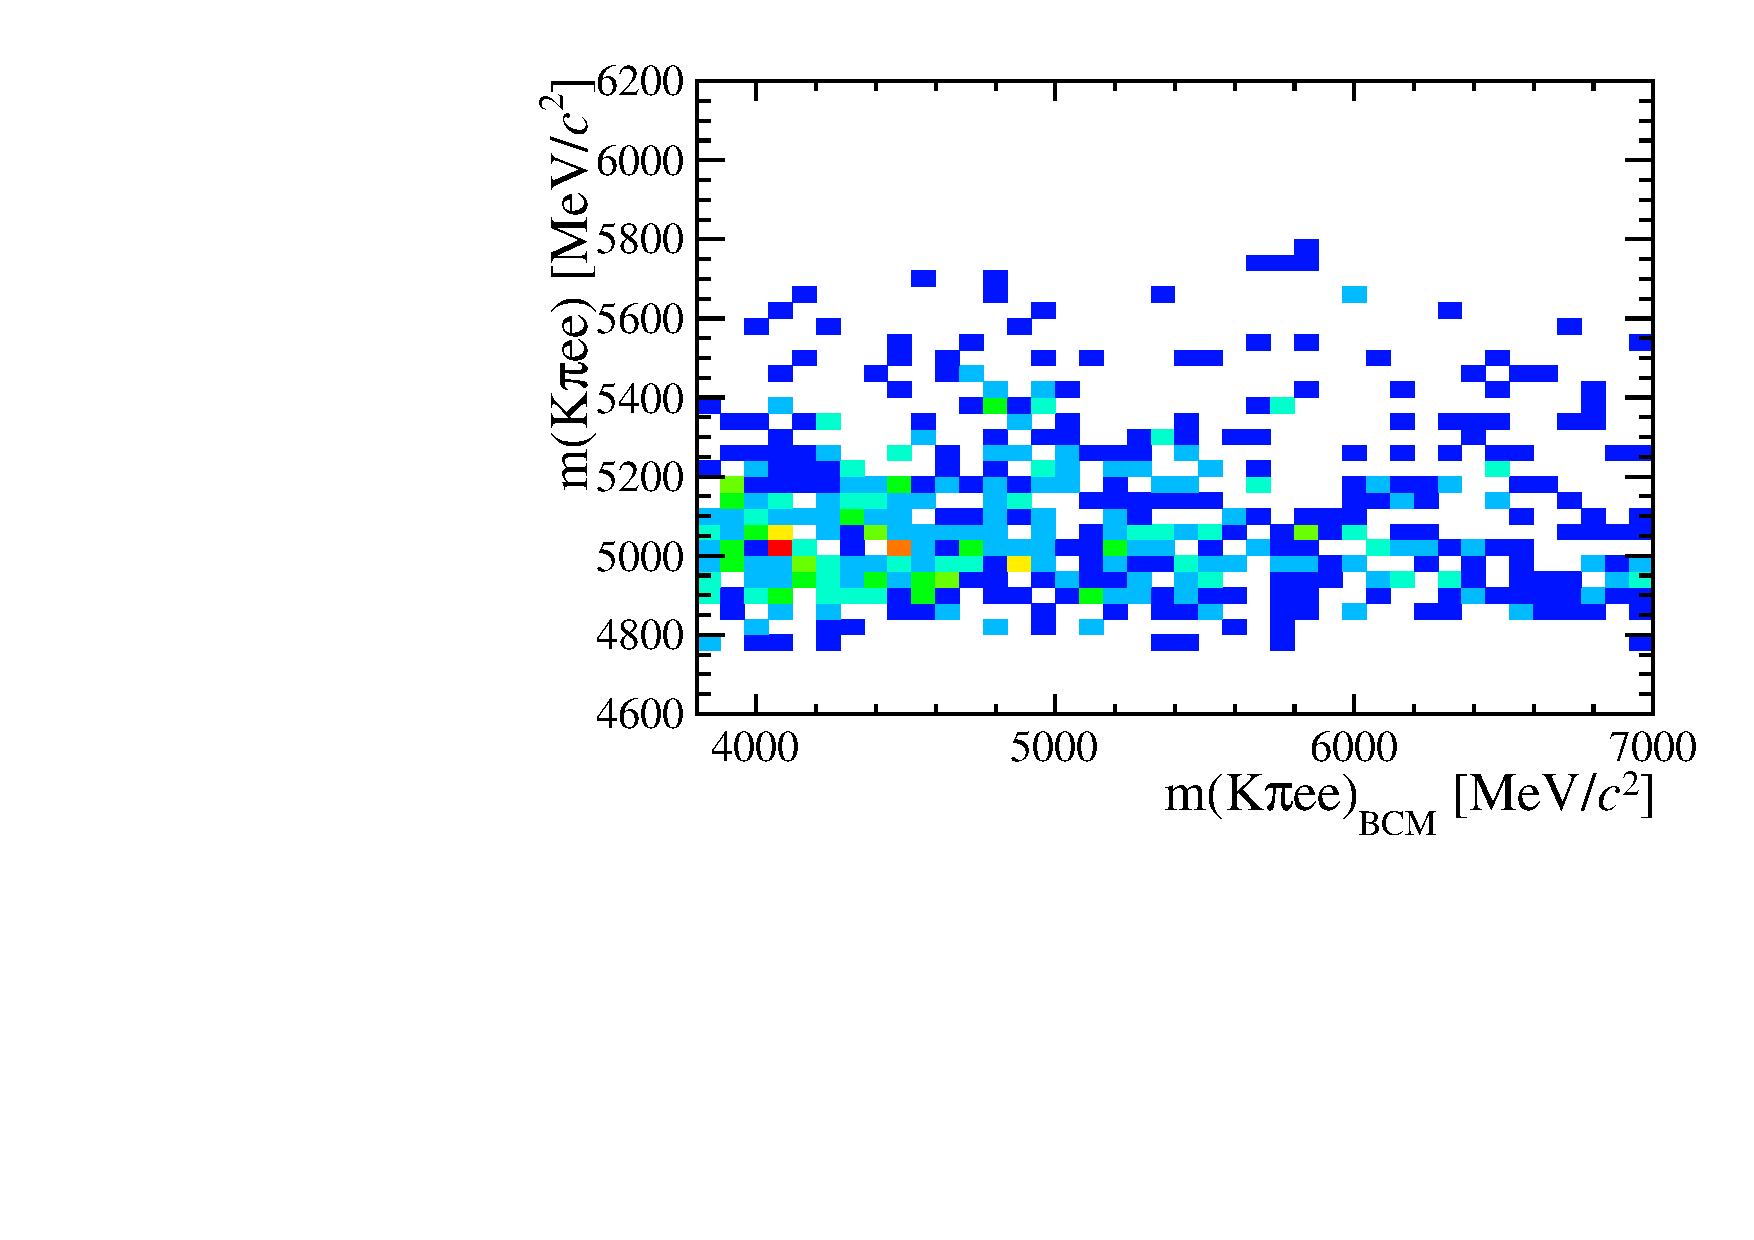
\includegraphics[width=0.48\textwidth]{RKst/figs/HOP/HOPvsM_bkg_high.pdf}
%\caption{Two-dimensional distribution of $m(K\pi ee) \vs \mbcm for (left) \BdToKstee signal and (right) partially-reconstructed background.
%From top to bottom the low-, central- and high-\qsq intervals.}
%\label{fig:hop2}
\end{figure}


\subsection{Multivariate analysis}
\label{sec:RKst_mva}

The final selection is performed using a neural network classifier based on the \mbox{\textsc{NeuroBayes}}
package~\cite{Feindt:2006pm,feindt-2004}. The multivariate analysis is intended to remove
some combinatorial background and obtain a clearer signal peak. In order to avoid biases, a so-called $k$-fold
approach is adopted to train and optimise the classifier, using $k=10$. In this method, the samples are divided into 
$k$ equally sized subsamples; $k$ classifiers are then trained and optimised each one using $(k-1)$ of the subsamples 
and applied to the $k$th one. This approach ensures that a classifier is never applied to the candidates used for its training.
Each classifier is trained on half of the candidates included in the $(k-1)$ subsamples and optimised using the other half,
which ensures that candidates used for training are not used for optimisation.

{\bf Samples:}

Representative samples of the signal and background are needed to train the classifier.
For the signal, fully reconstructed \BdToKstmm and \BdKstee simulated events can be used,
%The simulation is corrected improve the data-simulation agreement as described in (see Sec. \ref{sec:RKst_mc_weighting}).
while a sample representative of the background can be obtained using real data candidates
in the upper \Bz sideband: $m(K\pi\mu\mu) > 5400$~\mevcc~ and $m(K\pi ee) > 5600$~\mevcc.
The lower sideband is not used in the training as it contains a significant fraction of misreconstructed background.
All pre-selection requirements are applied to the samples used for the training.
As L0 and PID variables are not well described in simulation these cuts are not applied to the simulation
but their effect is taken into account by event weights.
%To train the classifier 50\% of the sideband events was used, keeping the other 50\% for testing.
An approximately equal number of signal and background candidates is used for the training
which corresponds to about $10^3$ electron and $10^4$ muon candidates.
%, which
%is driven by the amount of background available.

{\bf Training:}

The neural network input consists of 24 variables carrying information about the kinematics of the decays
and the quality of tracks and vertices. All the variables used are listed in Tab.~\ref{tab:RKst_mva_vars}.
% and their correlation is graphically represented in Fig.~\ref{fig:Rkst_nnCorrelation}.
%In these figures the variable with ID = 1 is the neural network output and the other IDs are reported in Tab.~\ref{tab:RKst_mva_vars}.
The single most discriminating variable is $\chisq_{\rm DTF}$, the \chisq of a kinematic fit (see Sec.~\ref{sec:DTF})
that constrains the decay product of the \Bz, the \Kstarz and the dilepton, to originate from their respective vertices.
Other variables that contribute significantly are the \chisqip of \jpsi and \Kstarz, the transverse momentum
of the \Bz and the pointing direction (\verb!DIRA!) of the reconstructed \Bz to the primary vertex.
%
%
\begin{table}
\centering
\caption{List of variables used as inputs for the neural network training.
%Next to each variable the ID number in brackets provides the index
%reported in the correlation matrices shown in Fig.~\ref{fig:Rkst_nnCorrelation}.
}
\begin{tabular}{$l|^l}
\rowstyle{\bfseries}
Particle 	& Variables \\ \hline
\Bz		& \pt, \quad \chisqip, \quad $\chisq_{\rm FD}$, \quad $\chisq_{vtx}/\text{ndf}$, \quad \texttt{DIRA}, \quad $\chisq_{\rm DTF}/\text{ndf}$ \\
\Kstarz	& \pt, \quad \chisqip, \quad $\chisq_{\rm FD}$, \quad $\chisq_{vtx}/\text{ndf}$, \quad \texttt{DIRA} \\
$h$		& $\mathrm{min},\mathrm{max}(p_{\textrm{T}, \kaon},p_{\textrm{T}, \pi})$, \quad $\mathrm{min},\mathrm{max}(\chi_{\textrm{IP}, \kaon}^{2},\chi_{\textrm{IP}, \pi}^{2})$ \\
$\ell\ell$	& \pt, \quad \chisqip, \quad $\chisq_{\rm FD}$, \quad $\chisq_{vtx}/\text{ndf}$, \quad \texttt{DIRA} \\
$\ell$	& $\mathrm{min},\mathrm{max}(p_{\textrm{T}, \ell^+},p_{\textrm{T}, \ell^-})$, \quad $\mathrm{min},\mathrm{max}(\chi_{\textrm{IP}, \ell^+}^{2},\chi_{\textrm{IP}, \ell^-}^{2})$ \\
%\Bz			& $\chi^2_{\rm DTF}/\text{ndf}$ [1], DIRA [19], $\chi^2_{\rm FD}$ [15], $\chi^2_{vtx}/\text{ndf}$ [12], \chisqip [14], \pt [7] \\
%\Kstar		& $\chi^2_{\rm FD}$ [21], $\chi^2_{vtx}/\text{ndf}$ [11], \chisqip [2], \pt [5] \\
%Dilepton	& $\chi^2_{\rm FD}$ [17], $\chi^2_{vtx}/\text{ndf}$ [13], \chisqip [20], \pt [6] \\
%$e$			& \chisqip [3][4], \pt [9][10]\\
%$\mu$		& \chisqip [14][15], \pt [9][10]\\
%K			& \chisqip [18], \pt [16]\\
%$\pi$		& \chisqip [22], \pt [8]\\
\end{tabular}
\label{tab:RKst_mva_vars}
\end{table}
%
\begin{figure}[b]
\centering
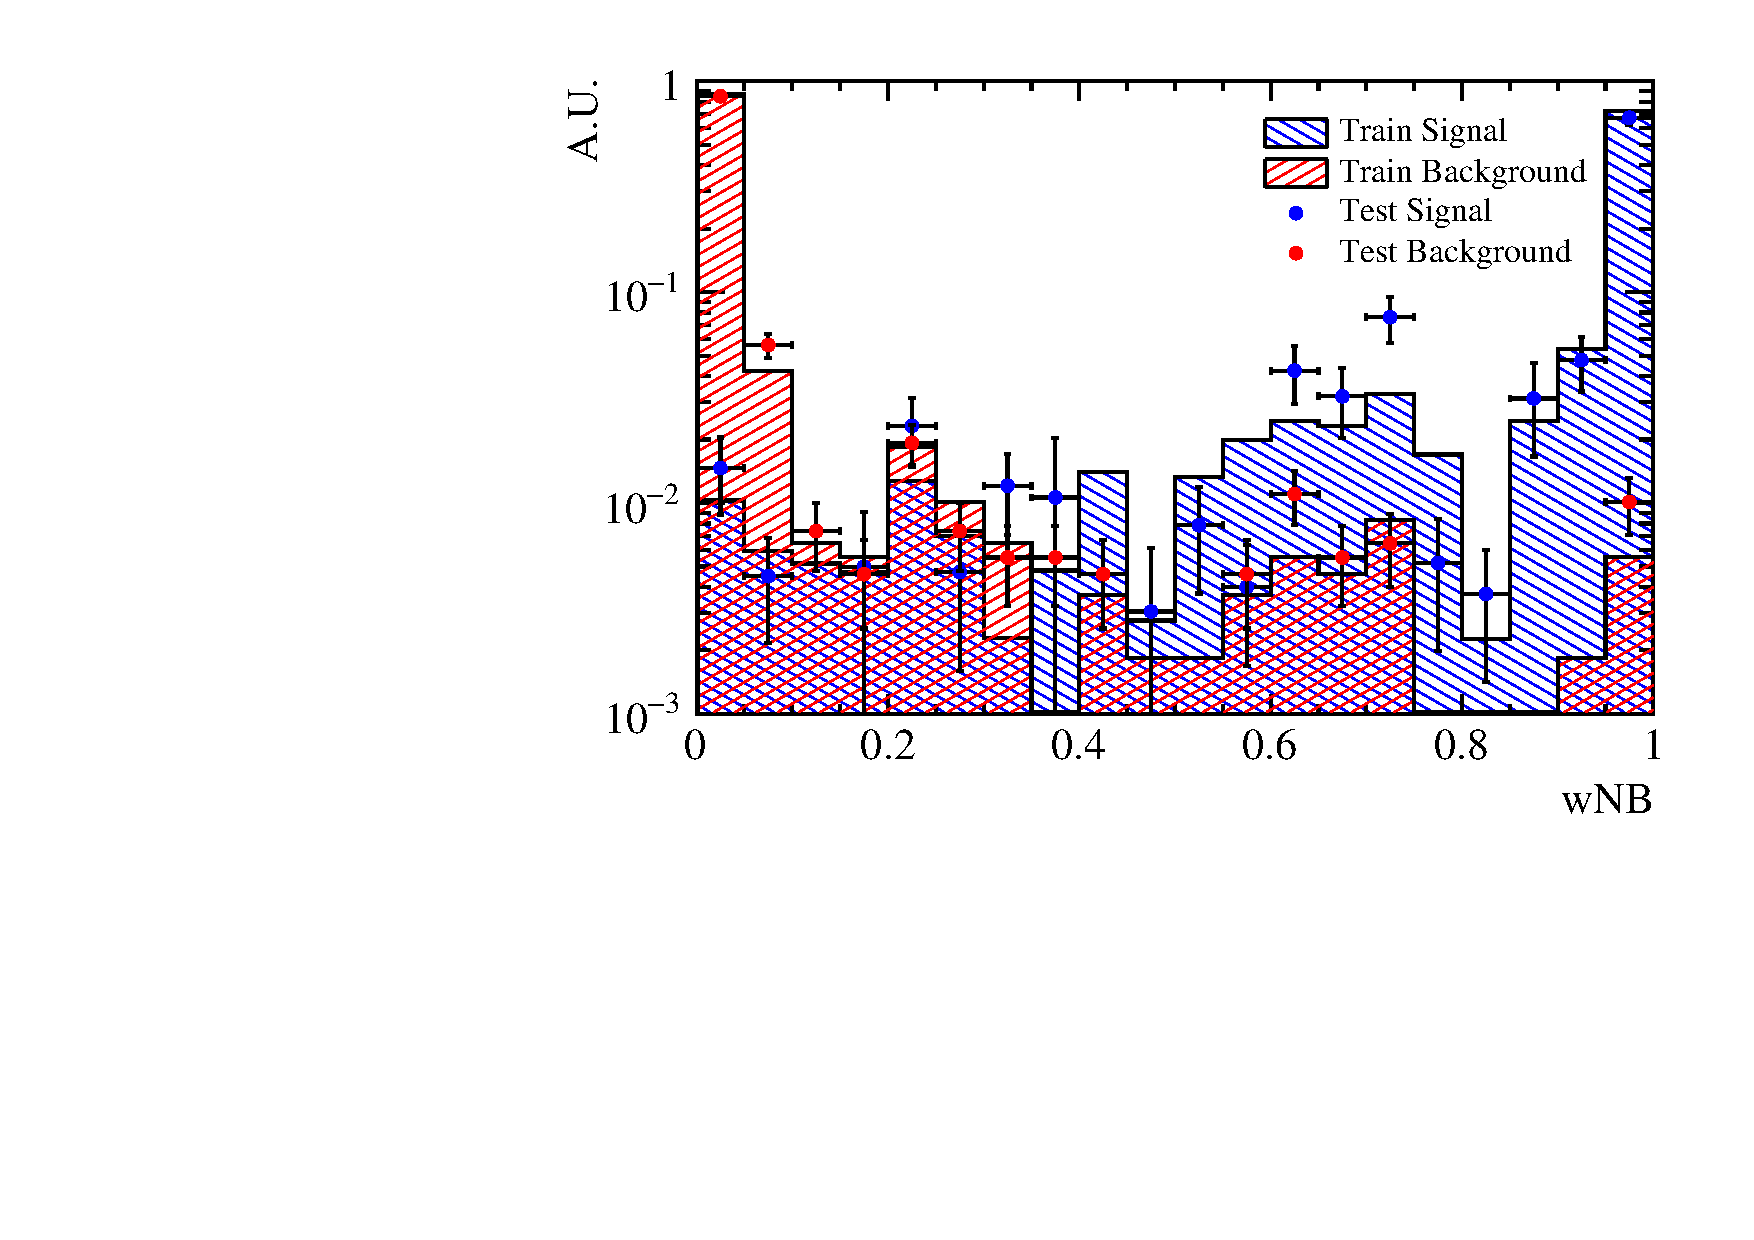
\includegraphics[width=0.49\textwidth]{RKst/figs/Training/EE_wNB_TrainAndTest.pdf}
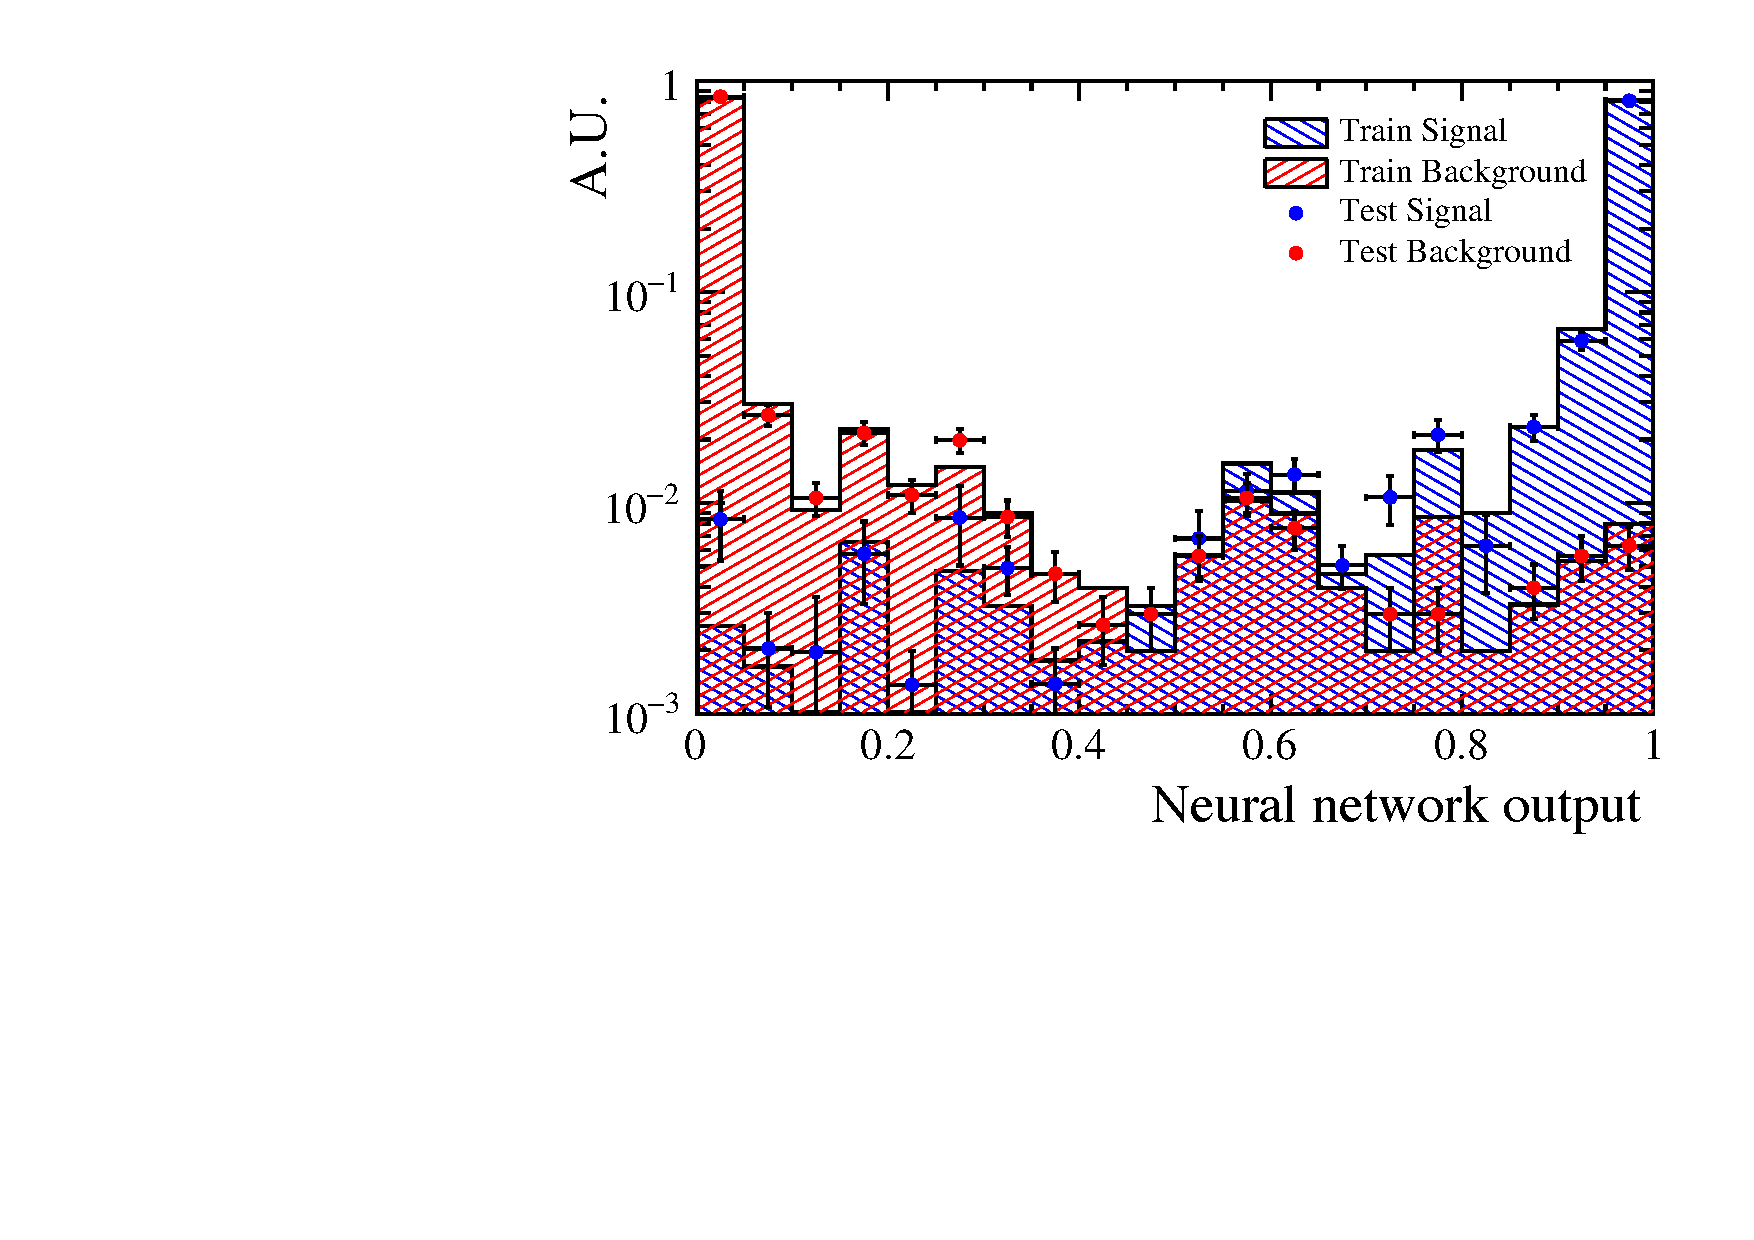
\includegraphics[width=0.49\textwidth]{RKst/figs/Training/MM_wNB_TrainAndTest.pdf}
\caption{Neural network output distributions for training (stripes) and test (points) samples, for simulated 
signal (blue) and data sideband (red) candidates. For the electron (left) and muon (right) training.}
\label{fig:RKst_nnDist}
\end{figure}
%
%The list the 5 most important variables is reported in Tab.~\ref{tab:RKst_nnInputs}, together
%with information on the relative importance of each input. The meaning of the column headings
%in this table was already explained in Sec.~\ref{sec:Lb_mva}.

%\begin{table}
%\centering
%\caption{Summary of inputs to the neural network in order of importance. The 5 most discriminating variables are shown.
%Column ``adds'' gives correlation significance added by given input when adding it to list of those
%ranked above, ``only this'' provides power of given input alone and ``loss'' shows how much information
%is lost when removing only given input. Decay Tree Fit is performed using DecayTreeFitter tool
%on whole decay chain with constraining tracks to appropriate vertex topology and the $m(p\pi)$
%invariant mass to the PDG value.}
%\begin{tabular}{c|ccc|c|ccc}
%\multicolumn{4}{c|}{Muons} 														& \multicolumn{4}{c}{Electrons}				%		  \\ \hline   
%Input                   			& Adds 			& Only this 	& Loss 			& Input        							& Adds      & Only this & Loss    \\ \hline
%$ \Bz$ $\chi^2_{\rm DTF}/\text{ndf} $		& 80.44 		& 80.44 		& 13.14  		&	$ \Bz$ $\chi^2_{\rm DTF}/\text{ndf} $		& 28.70 		& 28.70 		& 3.94  \\
%$ \Kstar$ $\chisqip $		& 22.26 		& 67.58 		& 3.48  		&	$ \Kstar$ $\chisqip $		& 12.71 		& 25.11 		& 1.57  \\
%$ \Bz\text{DIRA} $		& 10.58 		& 71.24 		& 3.95  		&	$ e_{2}$ $\chisqip $		& 6.56 		& 20.19 		& 3.30  \\
%$ \Kstar$ $\pt $		& 9.16 		& 49.13 		& 2.07  		&	$ e_{1}$ $\chisqip $		& 5.54 		& 19.66 		& 2.60  \\
%$ \jpsi$ $\chisqip $		& 6.58 		& 56.15 		& 1.35  		&	$ \Kstar$ $\pt $		& 3.74 		& 15.35 		& 3.14  \\
%$ \Bz$ $\pt $		& 6.00 		& 41.42 		& 4.39  		&	$ \jpsi$ $\pt $		& 4.81 		& 5.55 		& 3.18  \\
%$ \mu_{1}$ $\pt $		& 2.96 		& 15.85 		& 3.79  		&	$ \Bz$ $\pt $		& 2.78 		& 13.01 		& 2.20  \\
%$ \mu_{2}$ $\pt $		& 2.73 		& 15.04 		& 3.46  		&	$ \pi$ $\pt $		& 3.08 		& 7.93 		& 1.83  \\
%$ \jpsi$ $\pt $		& 3.06 		& 16.41 		& 2.84  		&	$ e_{2}$ $\pt $		& 2.35 		& 9.81 		& 2.74  \\
%$ \Kstar$ $\chi^2_{vtx}/\text{ndf} $		& 2.41 		& 28.14 		& 2.38  		&	$ e_{1}$ $\pt $		& 2.15 		& 8.04 		& 2.28  \\

%$ \Bz$ $\chi^2_{\rm FD} $		& 2.03 		& 63.73 		& 1.37  		&	$ \Kstar$ $\chi^2_{vtx}/\text{ndf} $		& 1.75 		& 7.45 		& 1.89  \\
%$ \mu_{1}$ $\chisqip $		& 1.45 		& 47.90 		& 1.75  		&	$ \Bz$ $\chi^2_{vtx}/\text{ndf} $		& 1.83 		& 27.54 		& 1.95  \\
%$ \mu_{2}$ $\chisqip $		& 1.04 		& 43.24 		& 1.20  		&	$ \jpsi$ $\chi^2_{vtx}/\text{ndf} $		& 1.10 		& 11.28 		& 1.16  \\
%$ K$ $\chisqip $		& 0.84 		& 62.99 		& 0.71  		&	$ \Bz$ $\chisqip $		& 1.11 		& 14.35 		& 1.24  \\
%$ \jpsi$ $\chi^2_{\rm FD} $		& 0.60 		& 55.41 		& 0.62  		&	$ \Bz$ $\chi^2_{\rm FD} $		& 0.93 		& 25.65 		& 1.21  \\
%$ \Bz$ $\chi^2_{vtx}/\text{ndf} $		& 0.56 		& 74.60 		& 0.61  		&	$ K$ $\pt $		& 0.82 		& 14.26 		& 0.61  \\
%$ \pi$ $\pt $		& 0.55 		& 34.94 		& 0.48  		&	$ \jpsi$ $\chi^2_{\rm FD} $		& 0.69 		& 23.85 		& 0.63  \\
%$ \Kstar$ $\chi^2_{\rm FD} $		& 0.34 		& 64.88 		& 0.41  		&	$ K$ $\chisqip $		& 0.56 		& 23.59 		& 0.52  \\
%$ \pi$ $\chisqip $		& 0.32 		& 56.92 		& 0.30  		&	$ \Bz\text{ $		& 0.53 		& 24.50 		& 0.52  \\
%$ \Bz$ $\chisqip $		& 0.30 		& 52.17 		& 0.30  		&	$ \jpsi$ $\chisqip $		& 0.37 		& 23.54 		& 0.38  \\
%$ \jpsi$ $\chi^2_{vtx}/\text{ndf} $		& 0.07 		& 18.35 		& 0.07  		&	$ \Kstar$ $\chi^2_{\rm FD} $		& 0.09 		& 23.66 		& 0.07  \\
%$ K$ $\pt $		& 0.03 		& 43.58 		& 0.03  		&	$ \pi$ $\chisqip $		& 0.01 		& 19.89 		& 0.01  \\
%\end{tabular}
%\label{tab:RKst_nnInputs}
%\end{table}

%\begin{figure}
%\centering
%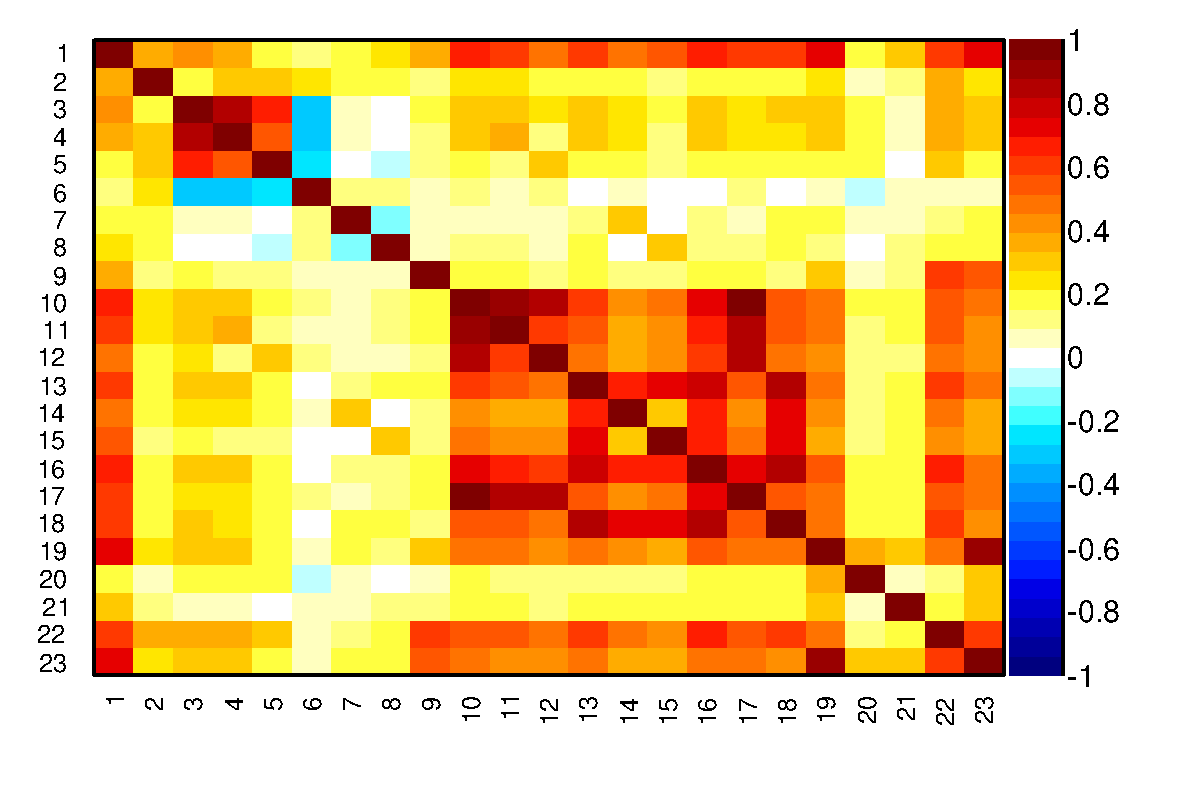
\includegraphics[width=0.8\textwidth]{RKst/figs/Training/electrons/correlation.pdf}
%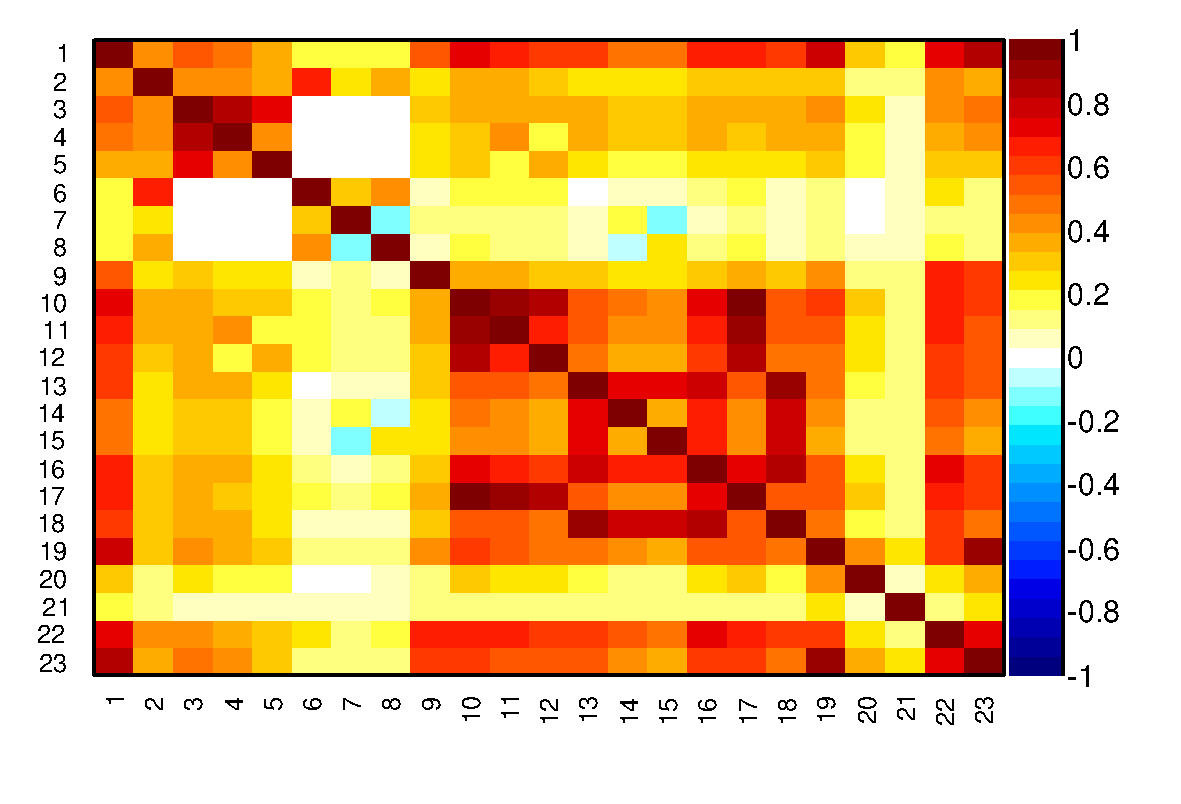
\includegraphics[width=0.8\textwidth]{RKst/figs/Training/muons/correlation.pdf}
%\caption{Graphical representation of correlation matrix between truth and neural network inputs.
%Column/row number 1 is correlation to the truth (whether candidate is signal or background). All
%others give correlation between inputs with numbering scheme corresponding to the id column of
%Tab.~\ref{tab:RKst_nnInputs}. Correlation is calculated using all events without distinguishing signal and
%background.}
%\label{fig:Rkst_nnCorrelation}
%\end{figure}
%

Figure~\ref{fig:RKst_nnDist} shows neural network output distributions for signal and background, with
the distributions from test samples overlaid in order to check for overtraining. 
The distributions follow the same shape but with different fluctuations indicating no
significant overtraining. In general it can be concluded that the neural network is able to separate signal
from background and that the training converged properly.

If too much information is given to the classifier, this can become able to calculate the invariant mass of the candidates 
from its input variables. This could generate a dependency of the efficiency on the 4-body invariant mass and it is therefore 
important to check for correlations between the invariant mass and the neural network output. Figure~\ref{fig:RKst_NNprofiles} 
shows the average neural network output as a function of the 4-body mass for sideband data and simulated signal candidates. 
The distributions are flat showing that no significant correlation is present.


\subsection{Optimisation}
\label{sec:optimisation}

\begin{figure}[t!]
\centering
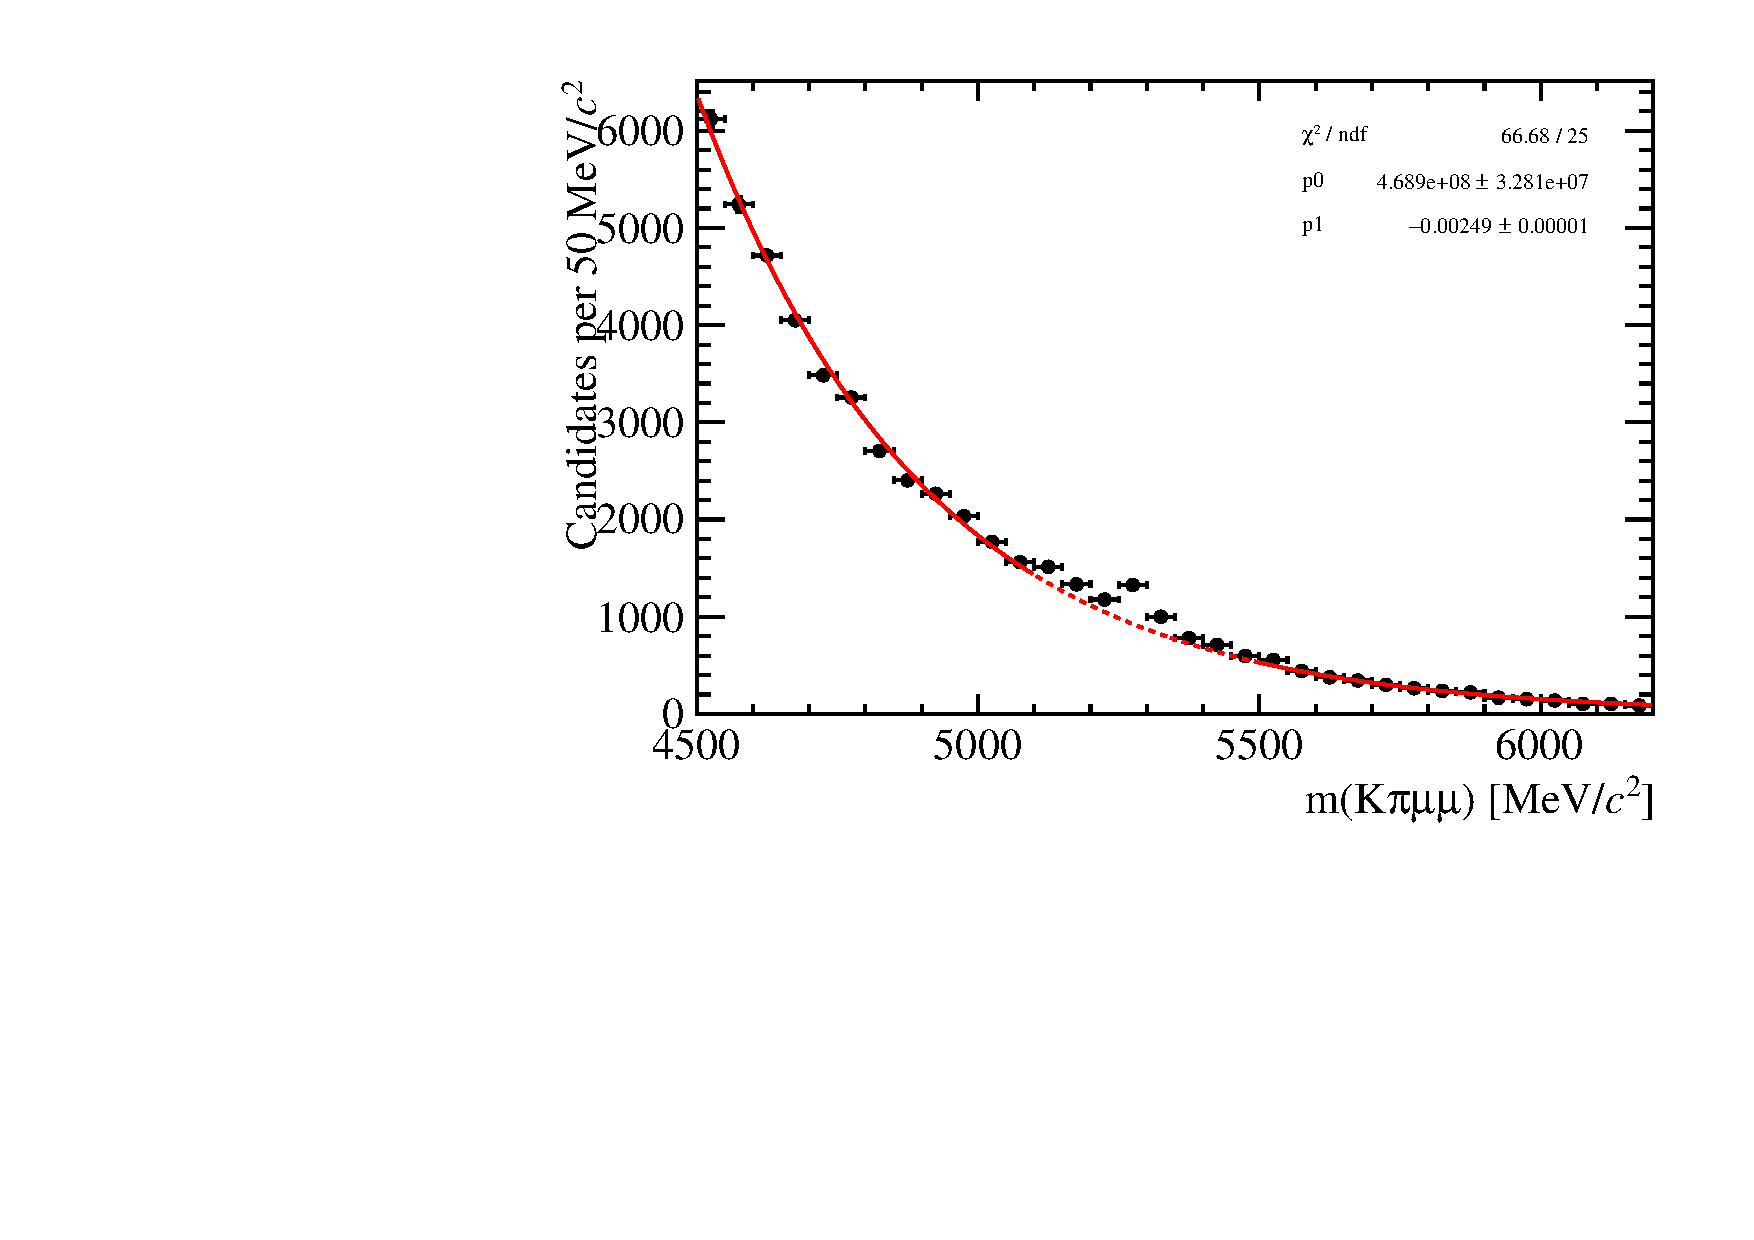
\includegraphics[width=0.49\textwidth]{RKst/figs/Optimisation/optimizeCut_MM-q2central/fitB_MM_0.pdf}
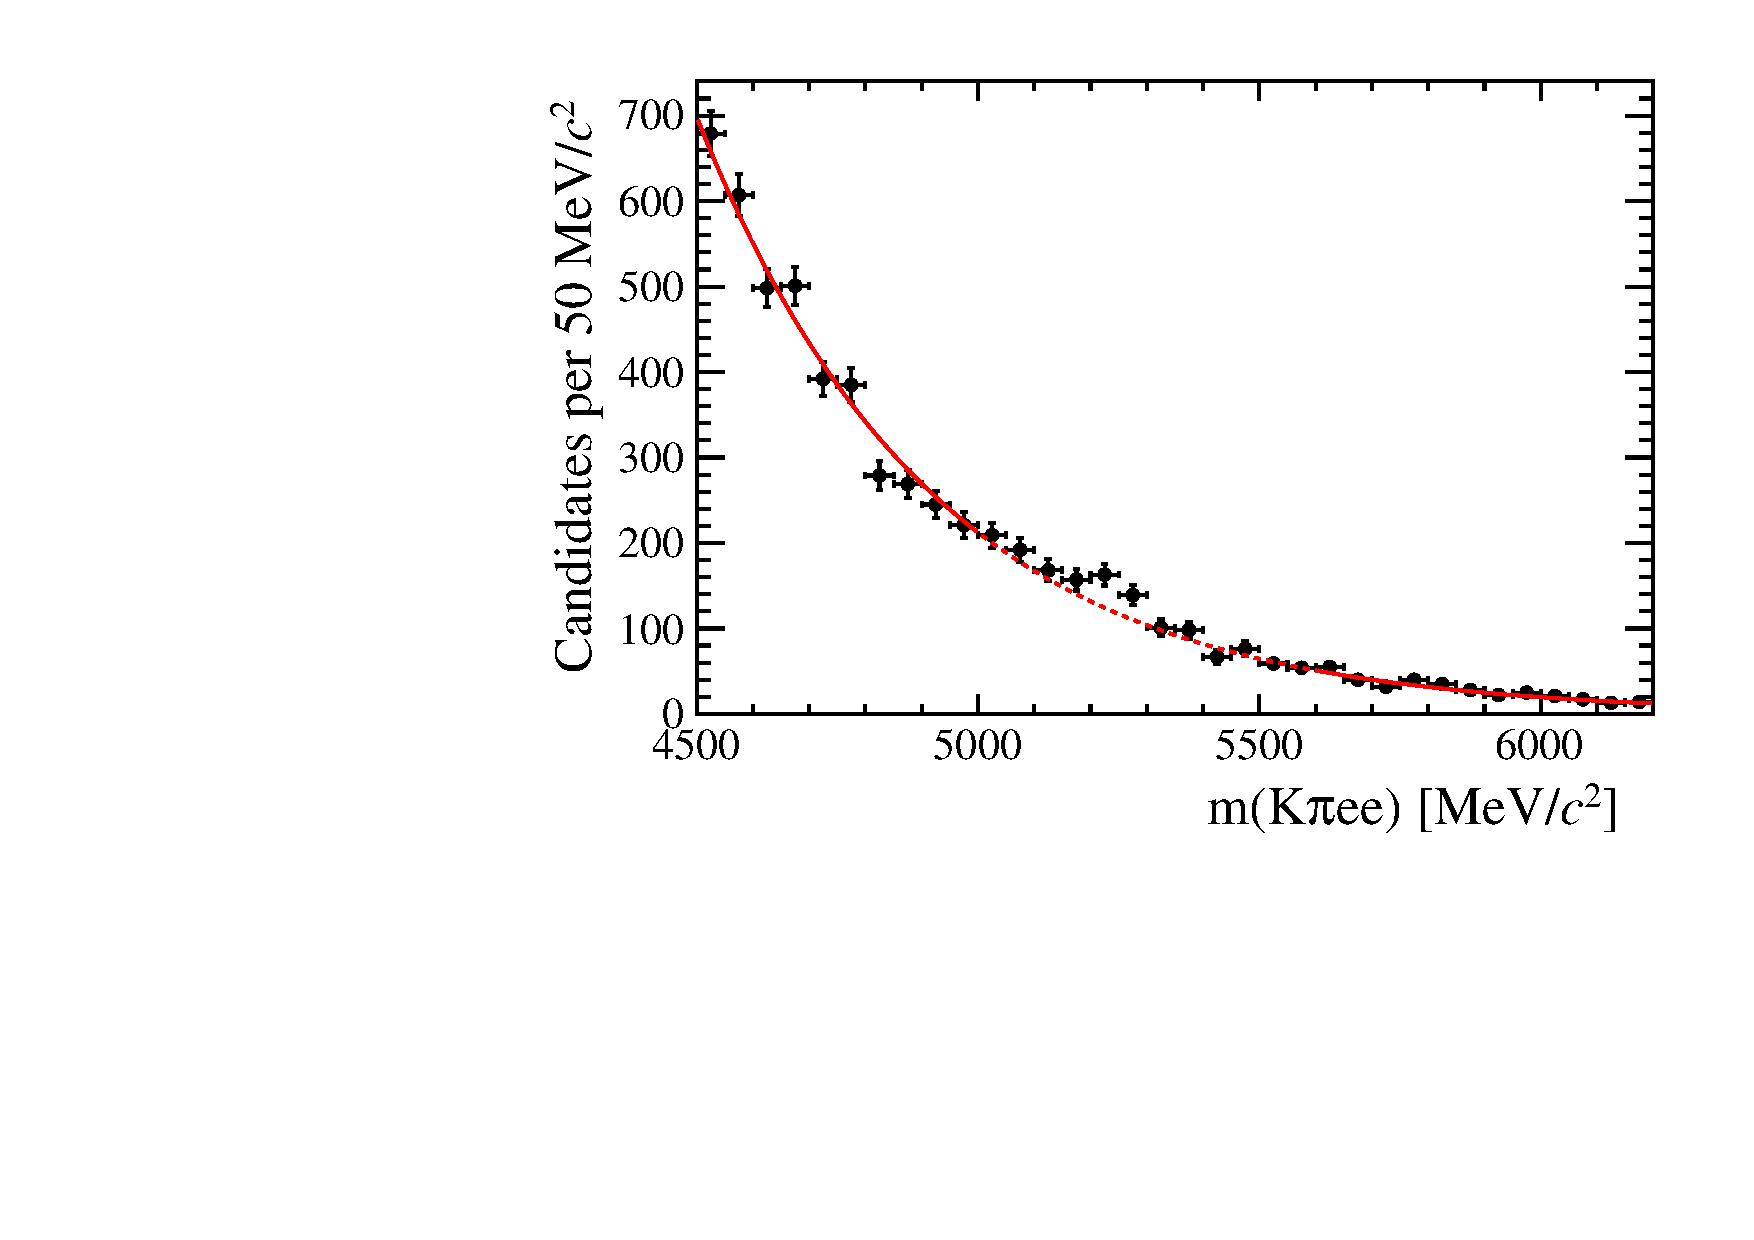
\includegraphics[width=0.49\textwidth]{RKst/figs/Optimisation/optimizeCut_EE-q2central/fitB_EE_0.pdf}
\caption{Fit to the data sidebands performed to estimate the amount of residual background in the
signal mass window for (left) muons and (right) electrons. The region corresponding to the dashed line is excluded from the fit.}
\label{fig:sideband_fit}
\end{figure}

In order to optimise the requirements on the \mbcm and the neural network output the expected
signal significance, $N_{\mathrm{S}}/\sqrt{N_{\mathrm{S}}+N_{\mathrm{B}}}$, is maximised,
where $N_\mathrm{S}$ ($N_\mathrm{B}$) is the number of rare signal (background) candidates.
When the BCM requirement is applied, the optimisation is performed in a three-dimensional space
($t_{\rm MVA}$, $a_{\rm BCM}$, $b_{\rm BCM}$), where $t_{\rm MVA}$ is the neural network output threshold below which
a candidate is considered background, and $a_{\rm BCM}$ and $b_{\rm BCM}$ are the parameters of the BCM
cut described in Sec.~\ref{sec:HOP}. Otherwise, only the MVA threshold is optimised 
(this is the case for all muons samples and the high-\qsq electron sample).

%The number of signal events accepted for a given neural network output cut is determined with a data-driven method
%with exploits the resonant channel. First, as an arbitrary number of events can be simulated, this has to be rescaled
%to the expected yield. This is done by fitting \decay{\Bz}{\Kstarz(\jpsi\to\ll)} candidates after pre-selection,
%including all requirements except MVA. The resonant yield is then scaled down by the expected ratio between
%the rare and the resonant channels. The number of background events is instead derived by fitting the combinatorial
%background in the sideband with an exponential function and extrapolating the fit function below the signal peak.

\begin{figure}[h!]
\centering
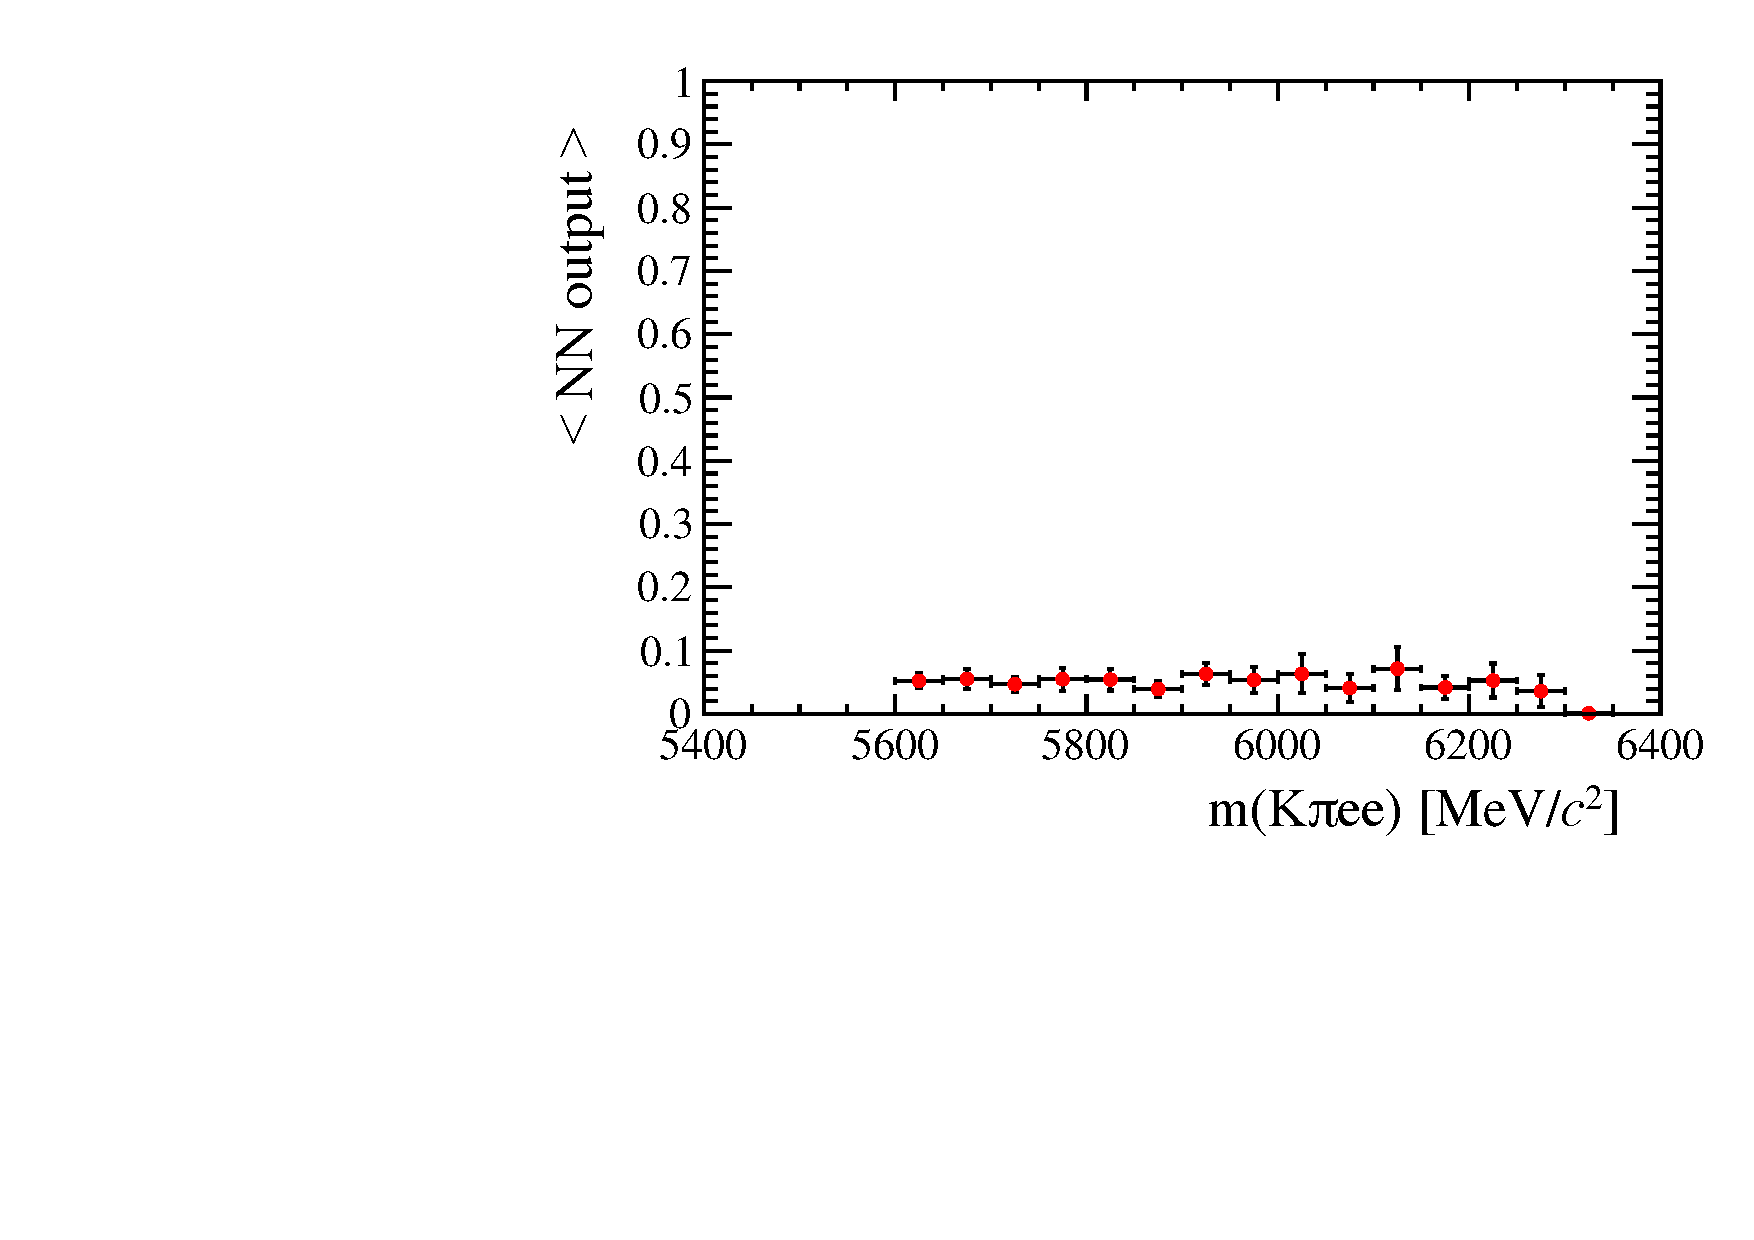
\includegraphics[width=0.49\textwidth]{RKst/figs/Training/EE_wNB_vs_MPV_bkg.pdf}
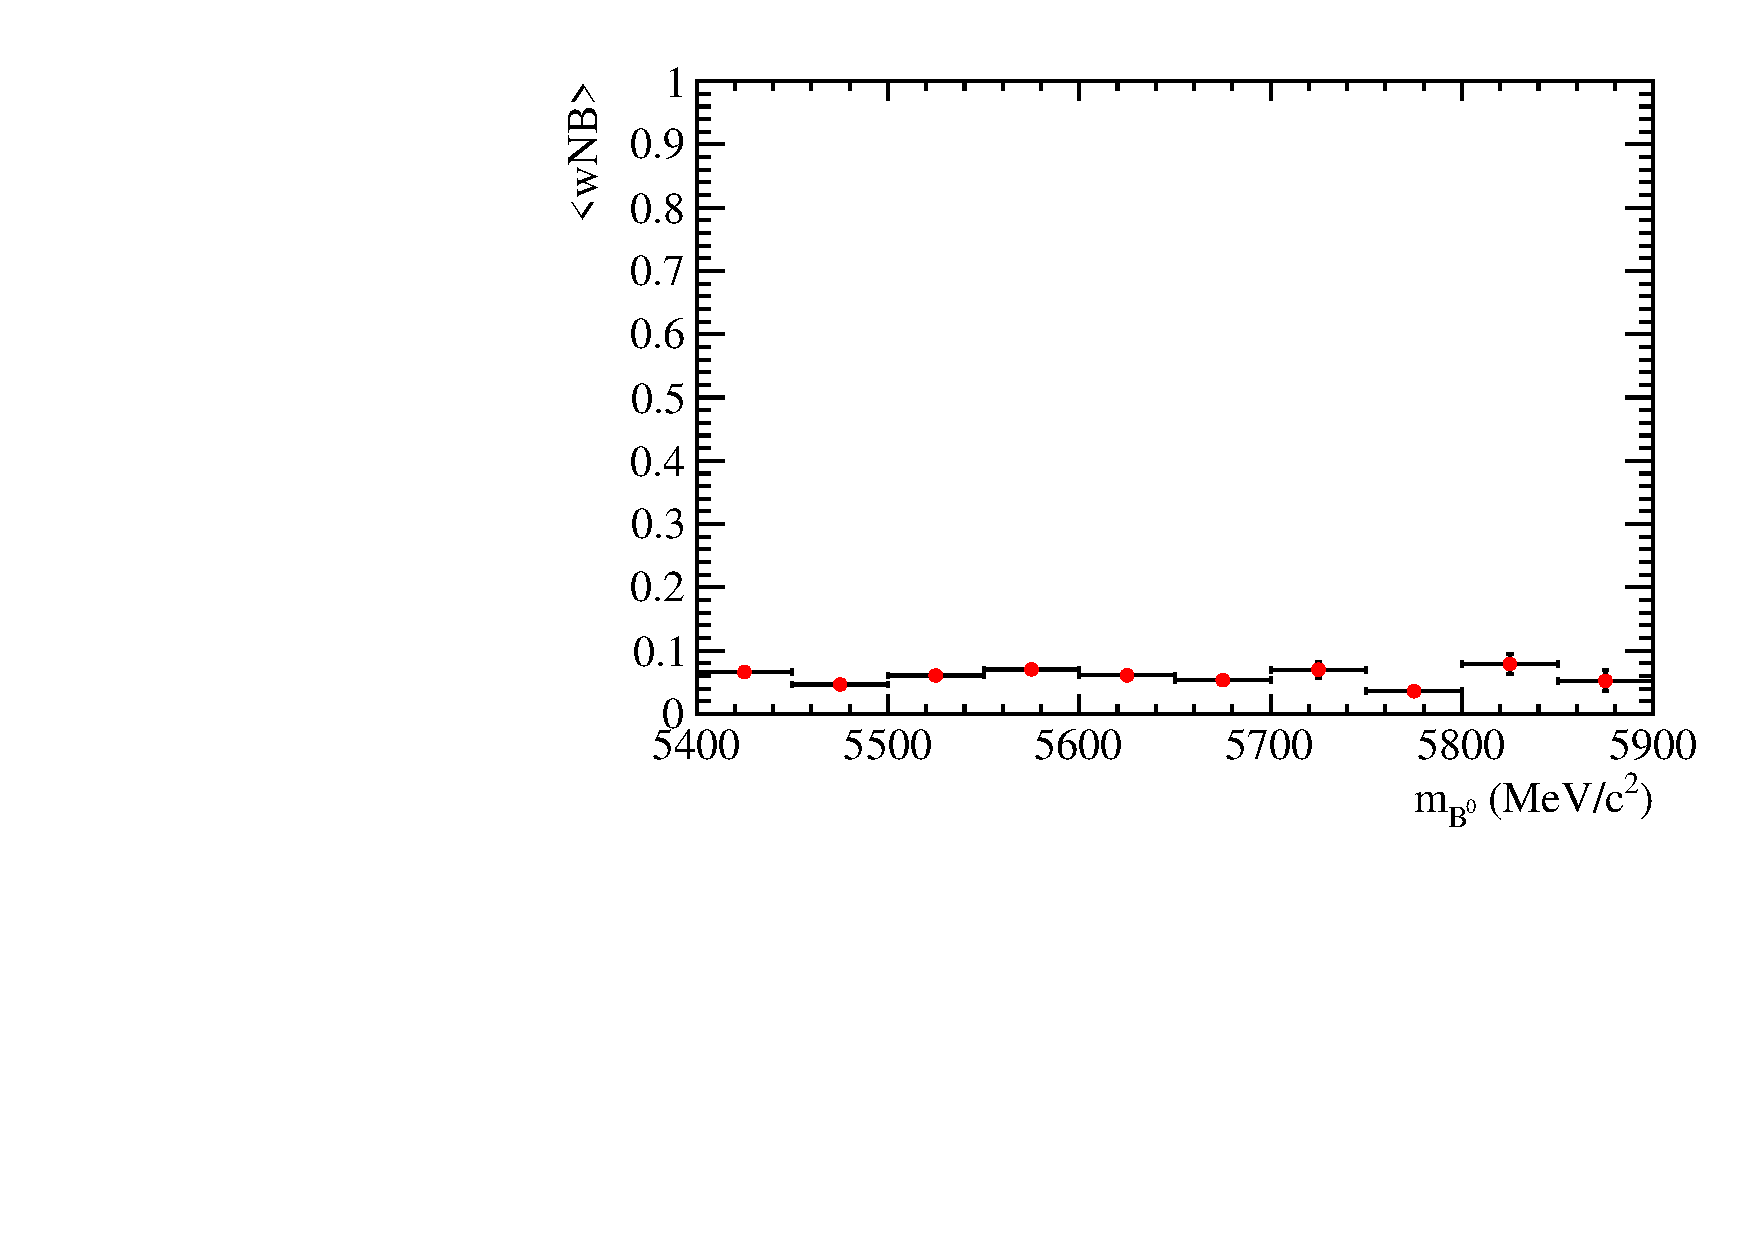
\includegraphics[width=0.49\textwidth]{RKst/figs/Training/MM_wNB_vs_MPV_bkg.pdf}
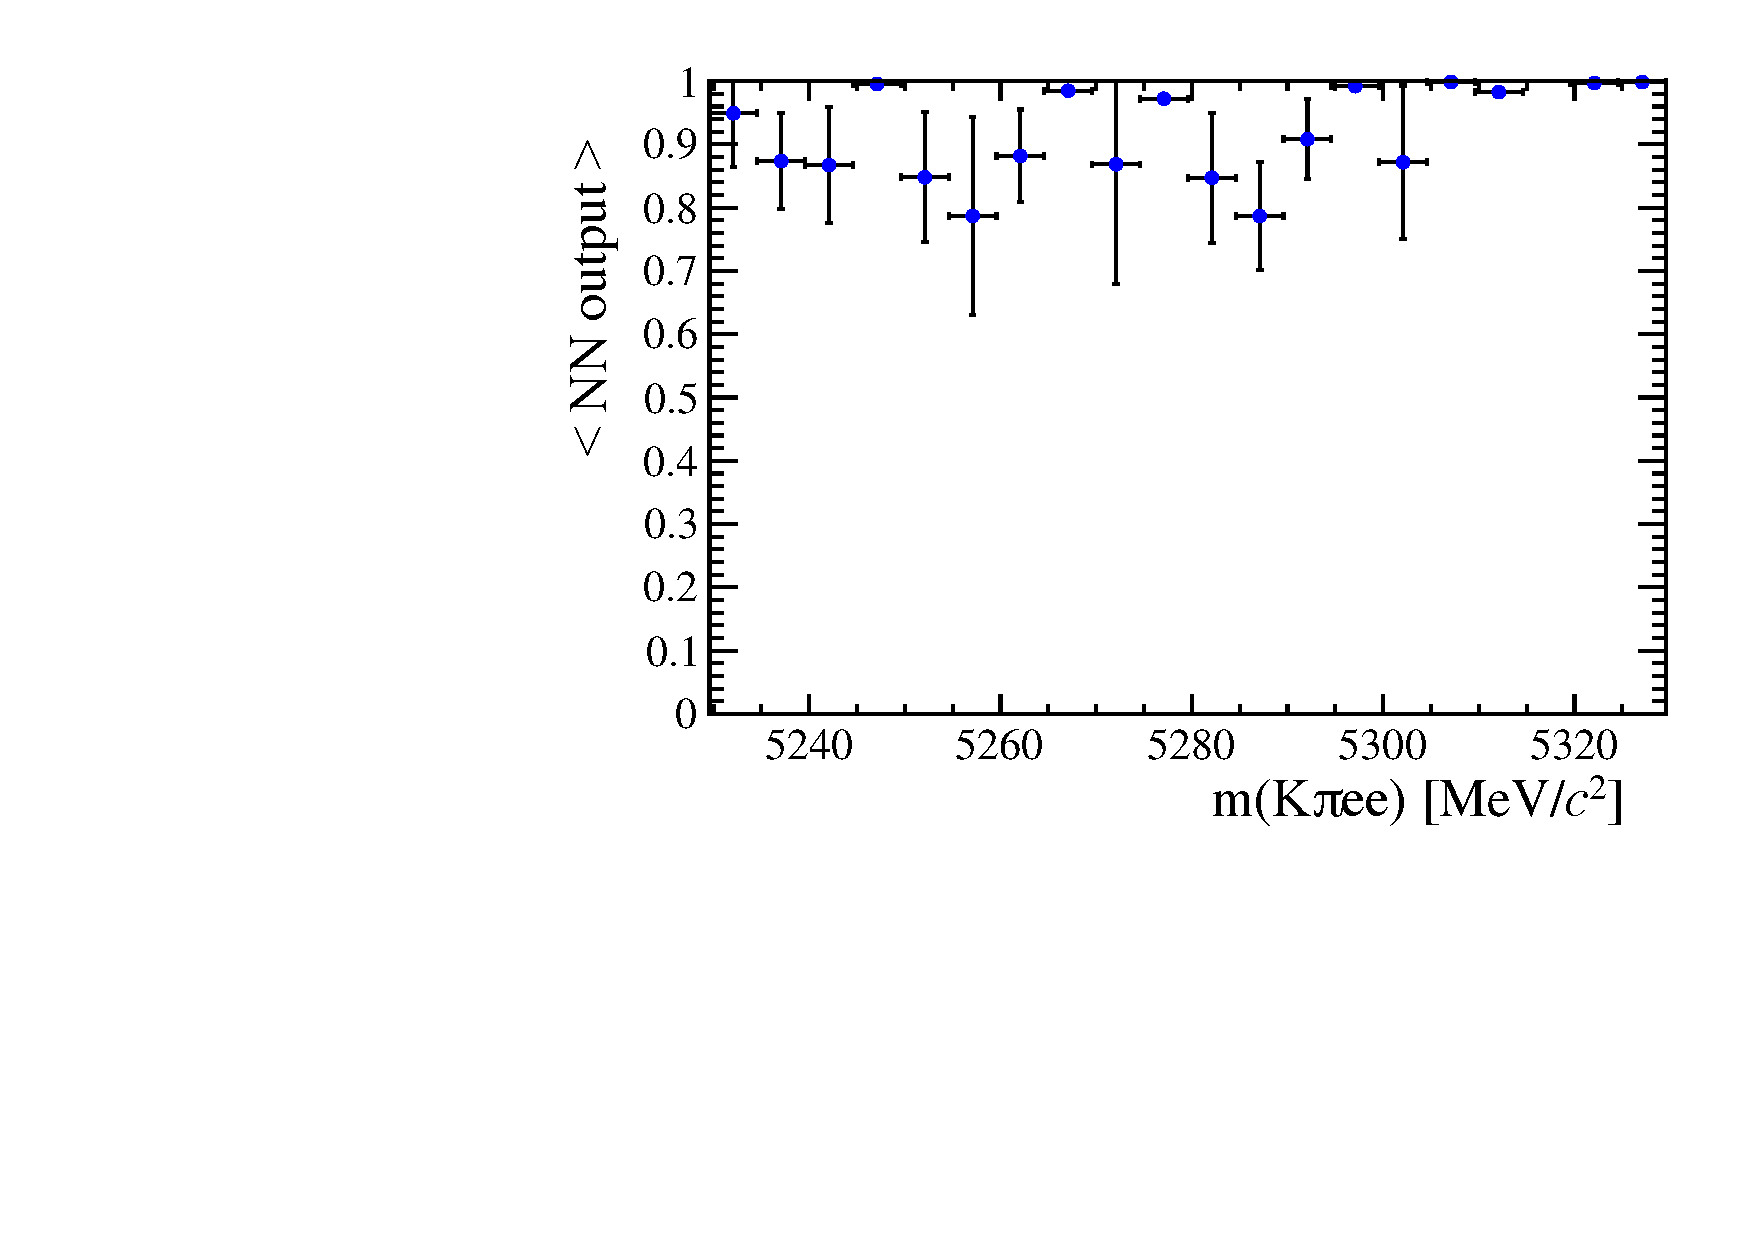
\includegraphics[width=0.49\textwidth]{RKst/figs/Training/EE_wNB_vs_MPV_sgn.pdf}
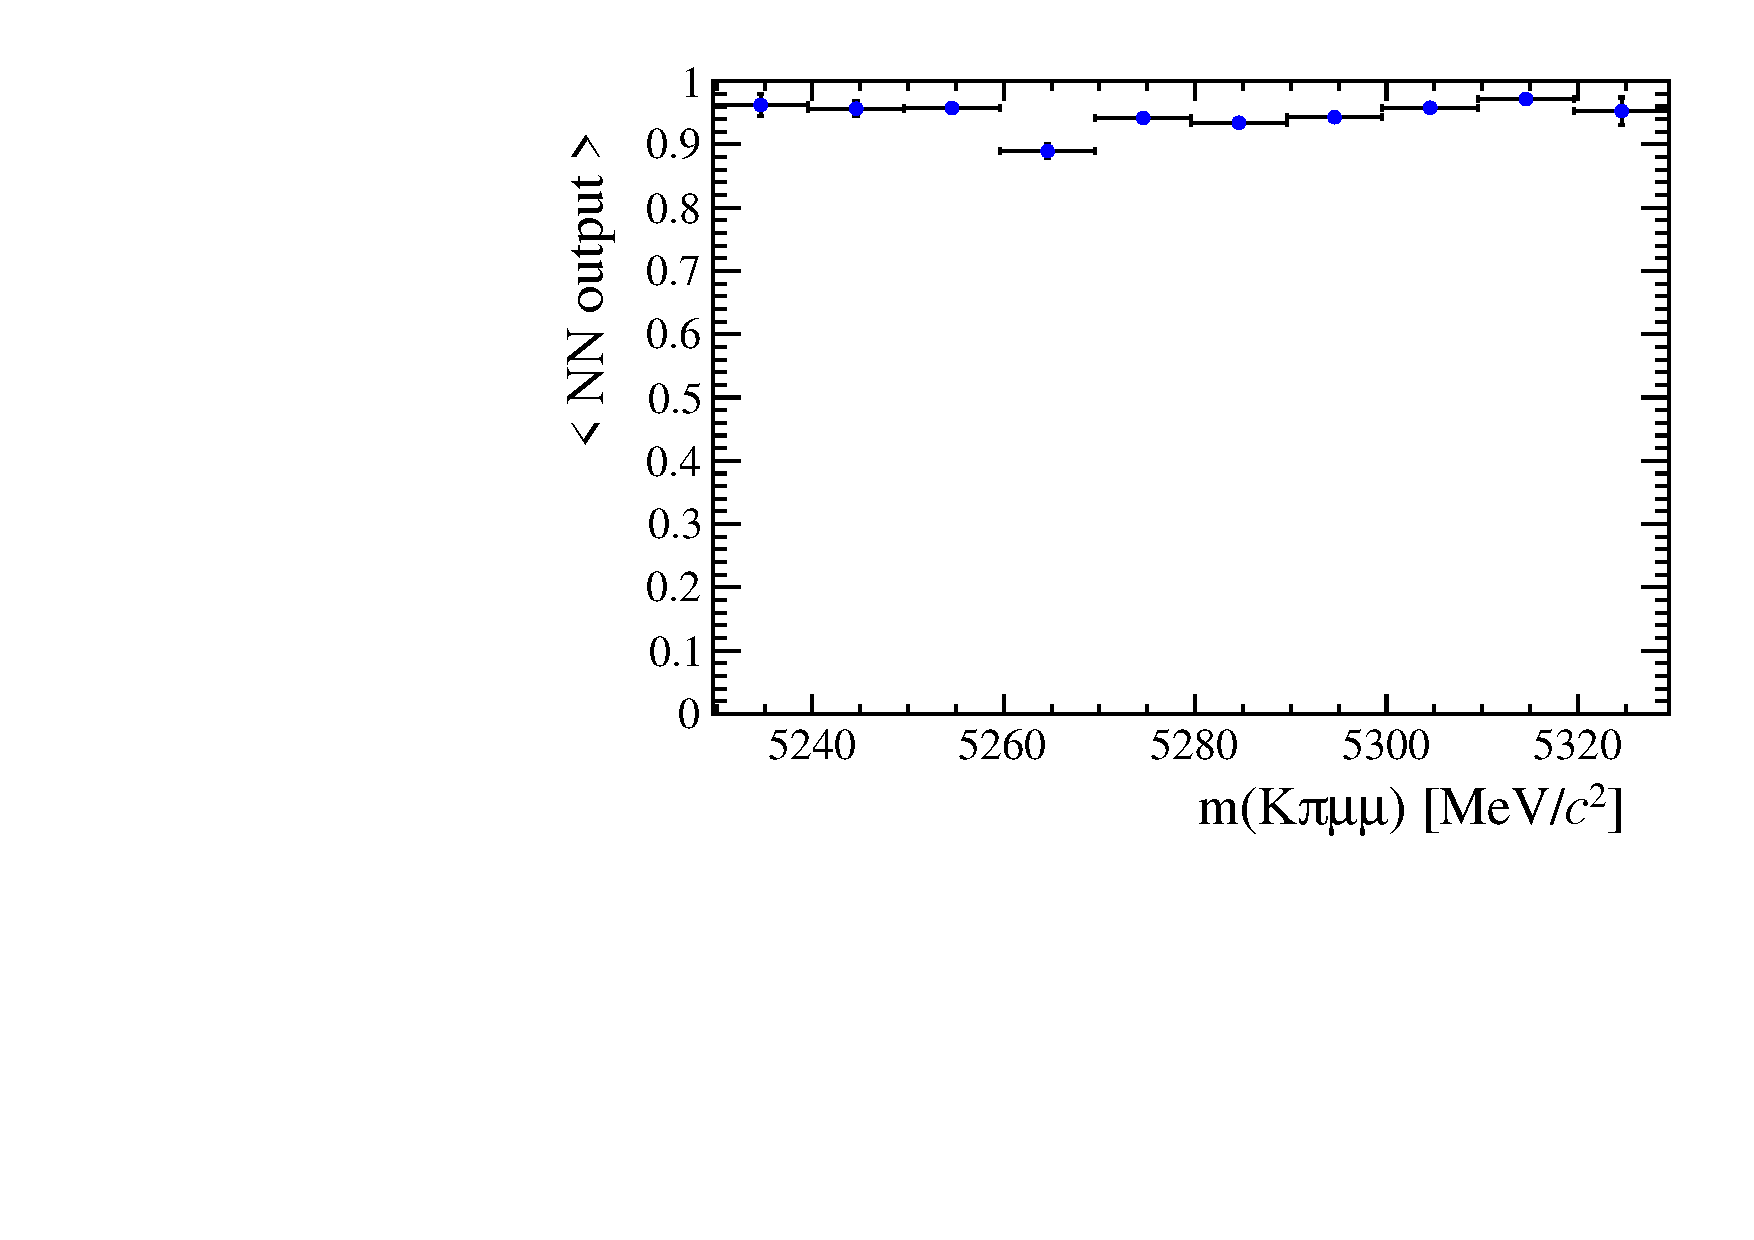
\includegraphics[width=0.49\textwidth]{RKst/figs/Training/MM_wNB_vs_MPV_sgn.pdf}
\caption{Average value of neural network output as a function of 4-body invariant mass for data
sideband (top) and simulated signal (bottom) candidates for the electron (left) and muon (right) trainings.}
\label{fig:RKst_NNprofiles}
\end{figure}
%
%
\begin{figure}[h!]
\centering
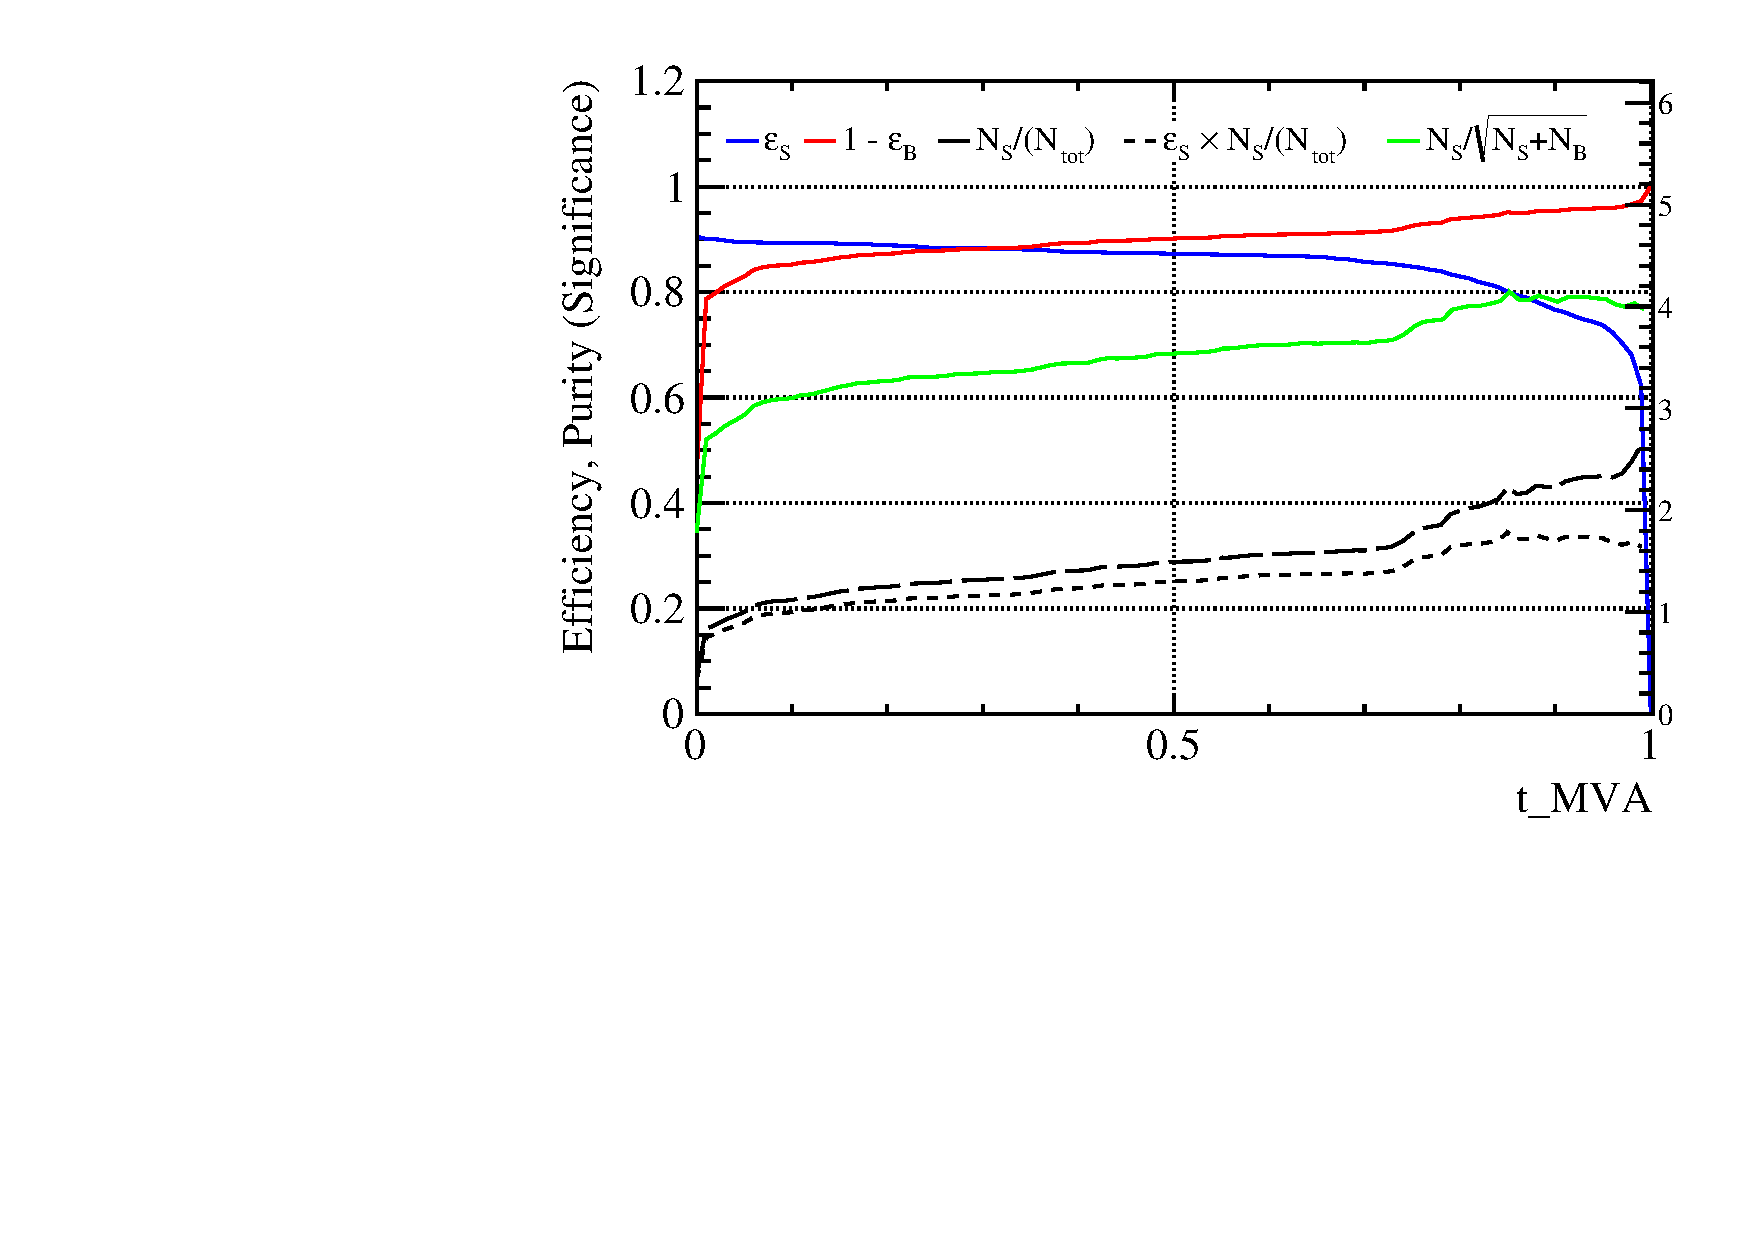
\includegraphics[width=0.49\textwidth]{RKst/figs/Optimisation/optimizeCut_EE-q2central/EE_Optimize_t_MVA.pdf}
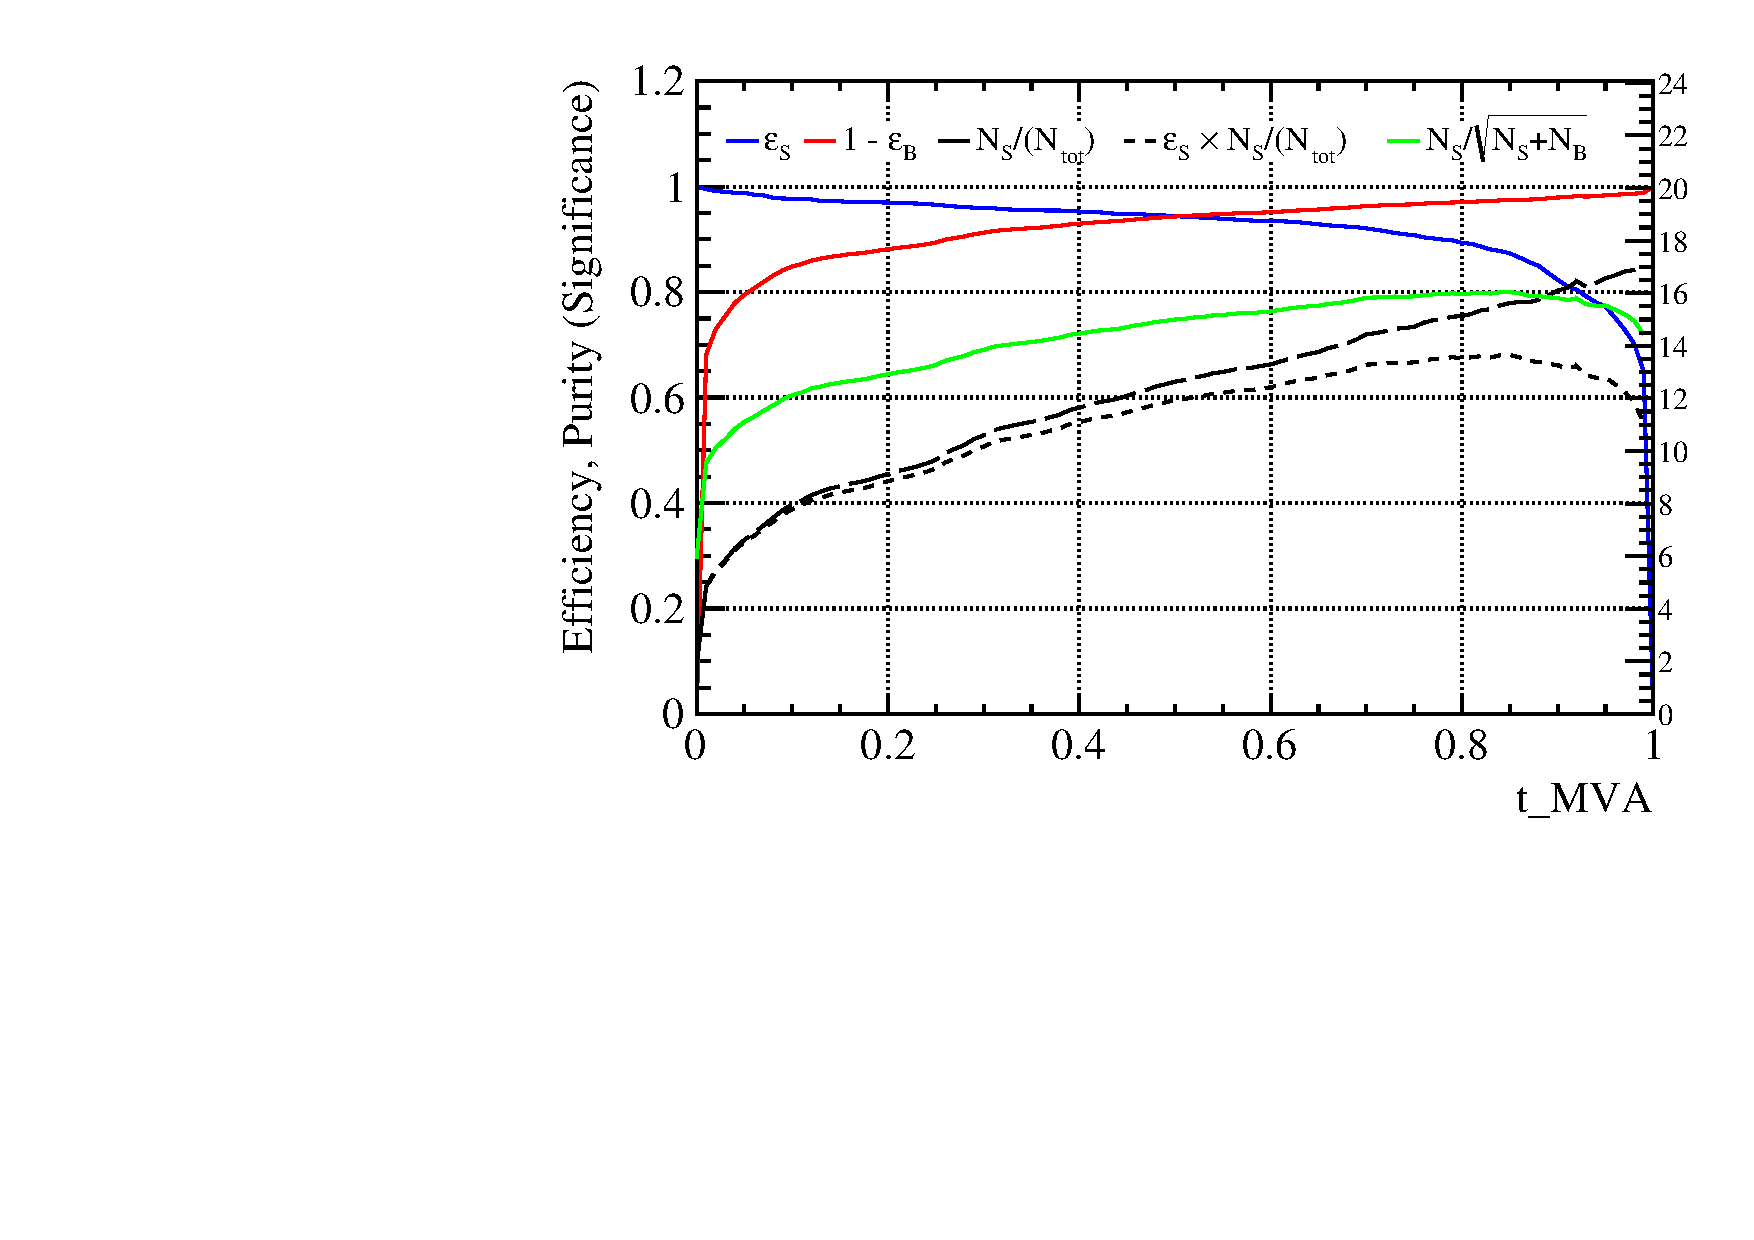
\includegraphics[width=0.49\textwidth]{RKst/figs/Optimisation/optimizeCut_MM-q2central/MM_Optimize_t_MVA.pdf}
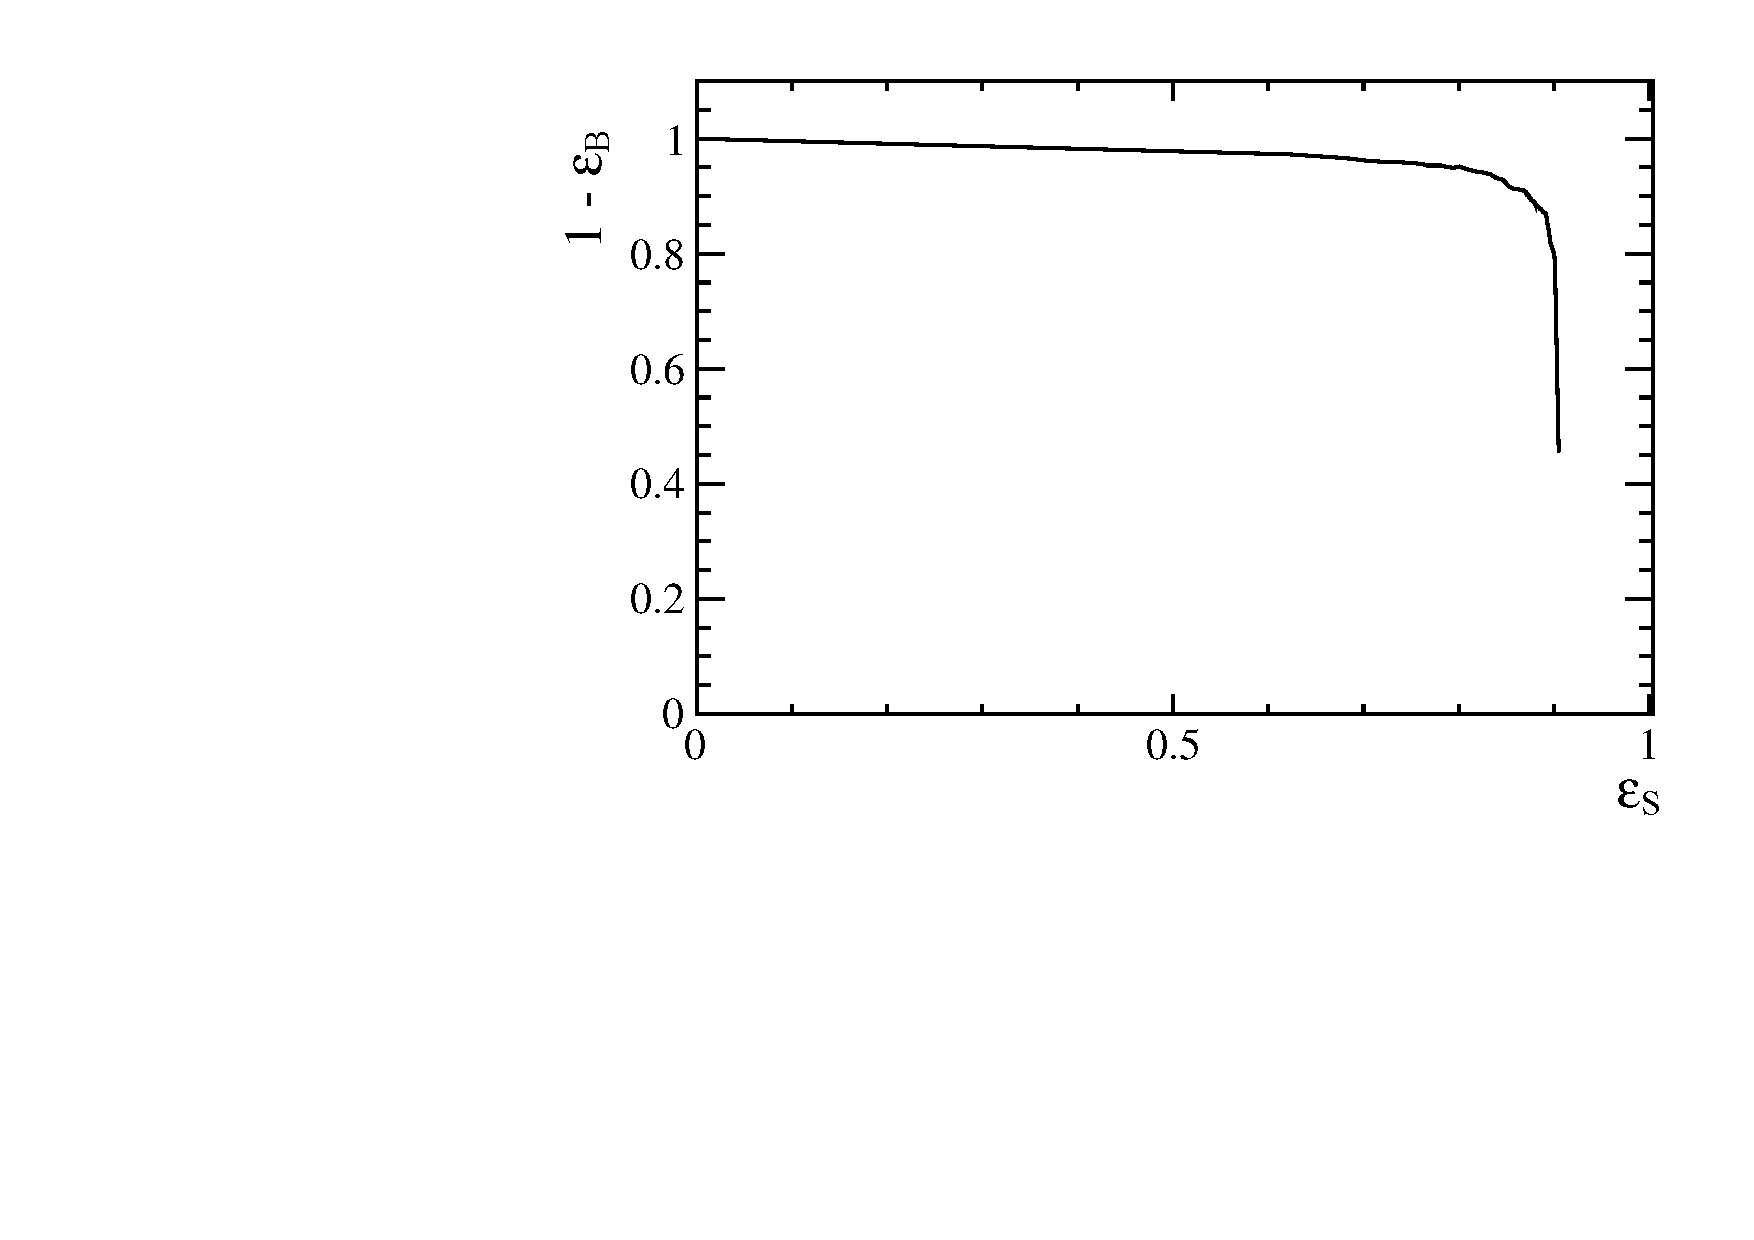
\includegraphics[width=0.49\textwidth]{RKst/figs/Optimisation/optimizeCut_EE-q2central/EE_ROC_t_MVA.pdf}
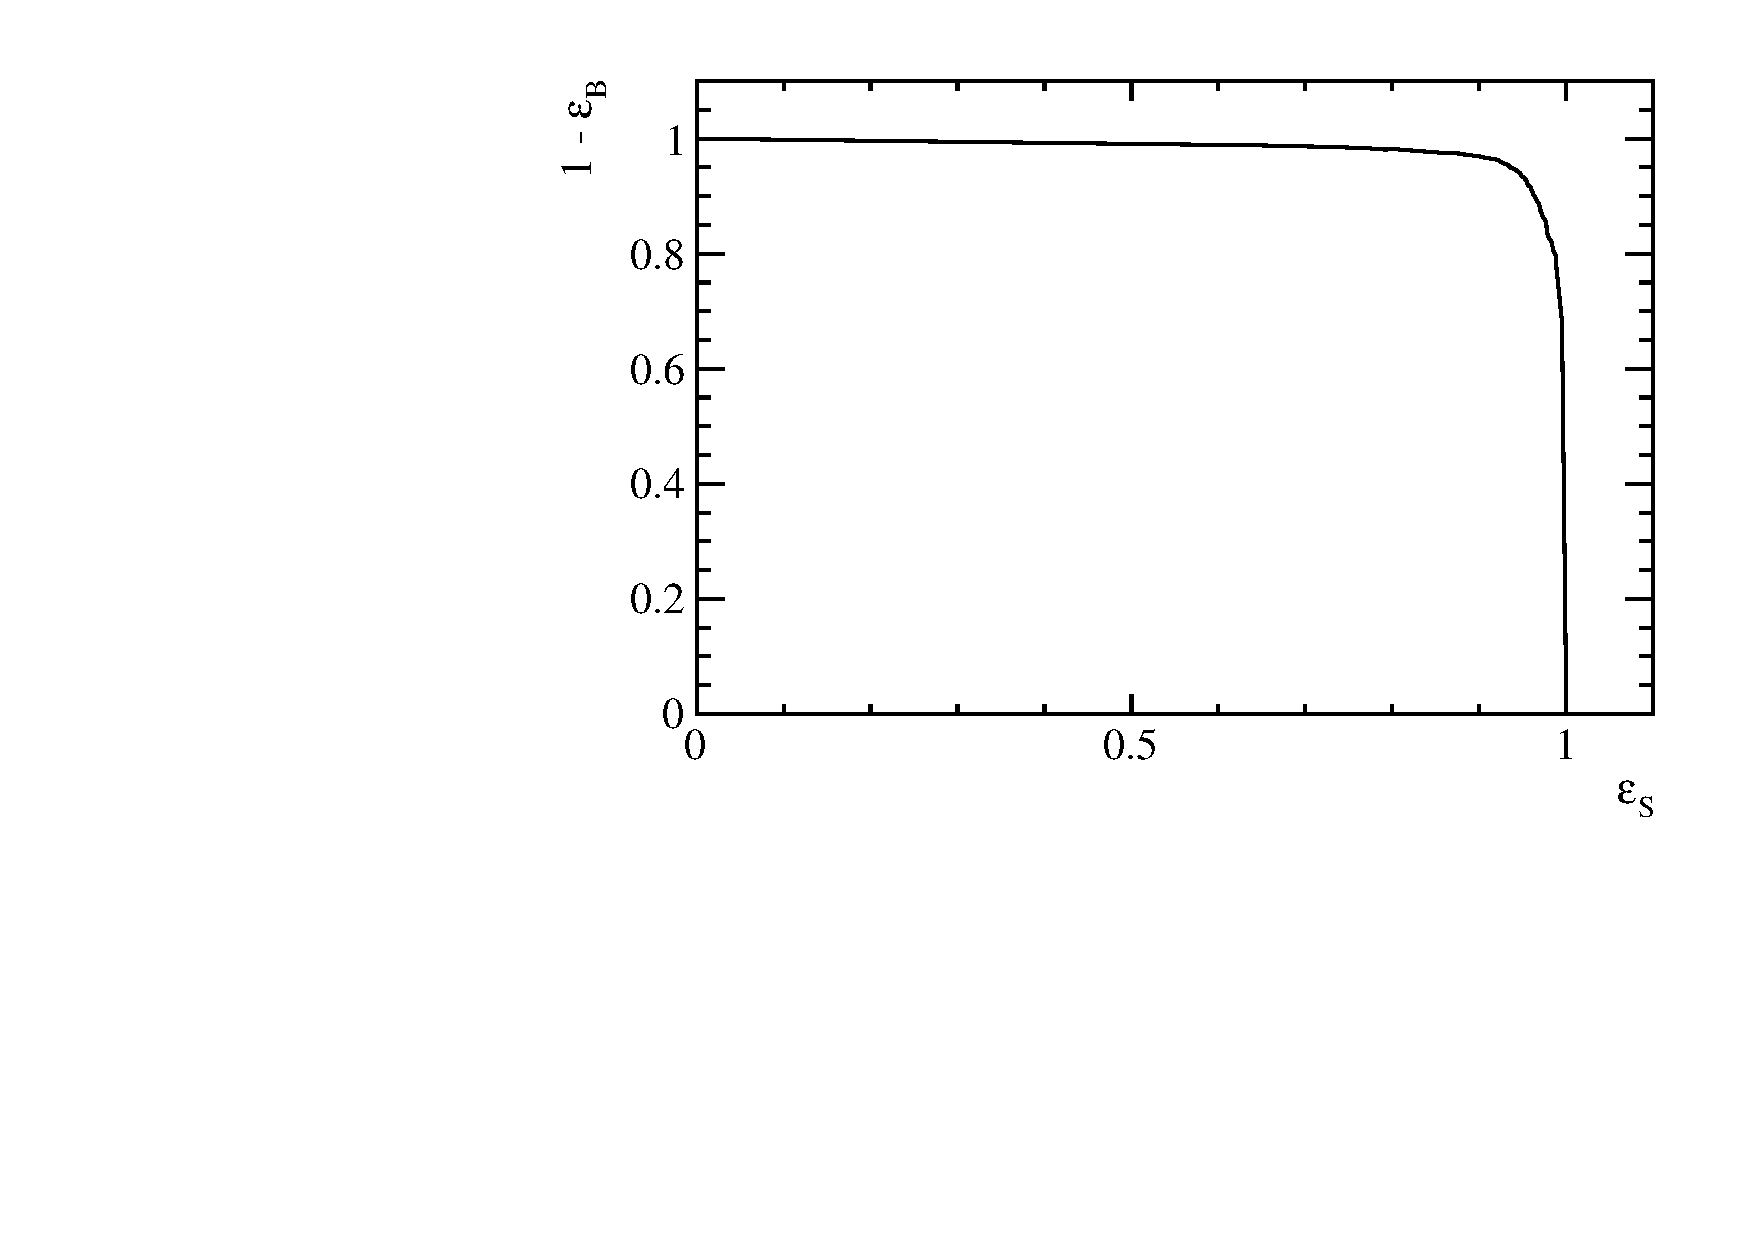
\includegraphics[width=0.49\textwidth]{RKst/figs/Optimisation/optimizeCut_MM-q2central/MM_ROC_t_MVA.pdf}
\caption{(top) Dependence of figure-of-merit on the requirement on neural network output.
(bottom) Signal efficiency versus background rejection.
Plots correspond to the electron (left) and muons (right) samples.}
\label{fig:RKst_FOM}
\end{figure}

The number of signal candidates accepted by a given requirement is determined using a data-driven method.
Firstly, \mbox{\BdToKstJPsll} candidates selected with all the requirements except for the MVA, and BCM cuts 
are fitted to determine the total yield. 
% (see Fig.~\ref{fig:RKst_sW_mass}).
This number is then scaled by the ratio of the rare and resonant branching fractions and
the efficiency ratio: 
%as a function of the cut
%
$$N_{\mathrm{S}} = N_{\jpsi(\ell\ell)} \cdot
\frac{\BR(\mathrm{\BdToKstll})}{\BR(\BdToKstJPsll)} \cdot
\frac{\varepsilon_{\mathrm{\ell\ell}}}{\varepsilon_{\jpsi(\ell\ell)}} \, .$$

The number of background candidates is also derived from data by fitting the background in the lower and upper 
mass sidebands with an exponential function, as shown in Fig.~\ref{fig:sideband_fit}, and extrapolating to obtain the residual yield into the signal region.
As the background shape changes as a function of the requirement that is being optimised, the sidebands are refitted for each considered cut value.
%
%$$N_{\mathrm{B}} \propto N_{\mKpill < 5000 \,||\, \mKpill > 5500} \, .$$

The optimisation is performed in a signal mass window of $\pm100~\mevcc$ around the nominal \Bz mass for muons, and between 5000 and 5400~\mevcc~ for electrons.
The average result of the $k$ optimisations is taken as the nominal requirement.
%
%
%
The variation of the signal and background efficiency, signal purity and figure-of-merit as a function of the neural network output
requirement for the central-\qsq is shown in Fig.~\ref{fig:RKst_FOM}
together with curves of the background rejection as a function of the signal efficiency.
%
%Using the described MVA cuts the signal efficiency is $\sim 95\%$ for the muon channels
%and $\sim 93\%$ for the electron channels (for more details see Sec.~\ref{sec:RKst_efficiency}),
%while the background rejections is $\sim 97\%$ on both samples.
%
After the full selection about $\sim 3\%$ of events still contain multiple candidates
which are removed at random to retain only a single candidate per event.

\clearpage

\subsection{Selection summary}

Table~\ref{tab:sel_summary} summarises the requirements applied for each sample 
on top of the pre-selection requirements described in Sec.~\ref{sec:RKst_trigstripping}.

\begin{table}[ht!]
\begin{center}
\caption{Summary of the selection requirements. The last column
indicates to  which \qsq intervals the requirement is applied.}
\label{tab:sel_summary}
\begin{footnotesize}
\renewcommand\arraystretch{1.4}
\begin{tabular}{c|c|c|c}
\multicolumn{2}{c|}{\textbf{Type}} & \textbf{Requirement} & {\boldmath\qsq} \\
\hline
\multirow{2}{*}{Quality} & \multirow{2}{*}{All tracks}
	& $\chisq_{trk}/\textrm{ndf} < 3$ & all \\
	&& {\verb GhostProb } $< 0.4$ & all \\
\hline
ID & \Kstarz & $|m(\kaon\pi) - m_{\Kstarz}^{PDG}| < 100\mevcc$ & all \\
\hline
 \multirow{4}{*}{PID}
	& $K$	& $\texttt{ProbNNk} \cdot (1 - \texttt{ProbNNp}) > 0.05$ & all \\
	& $\pi$	& $\texttt{ProbNNpi} \cdot (1 - \texttt{ProbNNk}) \cdot (1 - \texttt{ProbNNp}) > 0.1$ & all \\
	& $\mu$	& $\mathrm{min}(\texttt{ProbNNmu}) > 0.2$ & all $\mu\mu$ \\
	& $e$	& $\mathrm{min}(\texttt{ProbNNe}) > 0.2$ & all $ee$ \\
	\hline
	\multirow{19}{*}{BKG}
	& Swap & $|m((\decay{h}{\mu})\mu) - m_{\jpsi, (\psitwos)}^{PDG}| > 60\mevcc$ & all \\
	& \BuToKll & $\mathrm{max}(m(K\ell\ell),m((\decay{\pi}{\kaon})\ell\ell)) < 5.1\gevcc$ & all \\
	& \BsToPhill & $m(K(\decay{\pi}{K})) > 1040~\mevcc$ & all \\
	& \decay{\Bd}{\Dm\ep\nu} & $|\cos\theta_\ell\,| < 0.8$ & except high- \\
%	& \BdToKstGee & $\sigma_{Z}(\epem) < 30~\rm{mm}$ & only low- \\
	& \BdToKstG & $\sigma_{z}(\ee) < 30~\rm{mm}$ & except $\gamma(ee)$ \\
\cline{2-4}
	& \multirow{10}{*}{Comb}	& $\texttt{NNout} > 0.68$ & $\mu\mu$ low- \\
	&					& $\texttt{NNout} > 0.64$ & $ee$ low- \\
	& 					& $\texttt{NNout} > 0.85$ & $\mu\mu$ central- \\
	&					& $\texttt{NNout} > 0.97$ & $ee$ central- \\
	& 					& $\texttt{NNout} > 0.40$ & $\mu\mu$ high- \\
	&					& $\texttt{NNout} > 0.93$ & $ee$ high- \\
\cline{3-4}
	& 					& $\texttt{NNout} > 0.06$ & $\jpsi(\mu\mu)$ \\
	&					& $\texttt{NNout} > 0.20$ & $\jpsi(ee)$\\
\cline{3-4}
	&					& $\texttt{NNout} > 0.16$ & $\gamma(ee)$ \\
%	&					& $\texttt{NNout} > 0.36$ & \JPsee \mKpiee \\
	&					& $\texttt{NNout} > 0.68$ & $\psitwos(ee)$ \\
\cline{2-4}
	& Part-reco					& $m(K\pi\ell\ell)_\jpsi	> 5150$~\mevcc		& $\jpsi(ee)$	\\
\cline{2-4}
	& \multirow{3}{*}{Comb, part-reco}	& $\mbcm > 4680 + 31 \cdot \log(\chisq_{\rm FD})$ & $ee$ low- \\
	&							& $\mbcm > 4437 + 64 \cdot \log(\chisq_{\rm FD})$ & $ee$ central- \\
\cline{3-4}	
	&							& $\mbcm > 3380 + 140 \cdot \log(\chisq_{\rm FD})$ & $\gamma(ee)$ \\
%	&							& $\mbcm > 2714 + 164 \cdot \log(\chisq_{\rm FD})$ & $\jpsi(ee)$ \\	
\end{tabular}
\end{footnotesize}
\end{center}
\end{table}


